% This work is licensed under the Creative Commons
% Attribution-NonCommercial-ShareAlike 4.0 International License. To view a copy
% of this license, visit http://creativecommons.org/licenses/by-nc-sa/4.0/ or
% send a letter to Creative Commons, PO Box 1866, Mountain View, CA 94042, USA.

% (c) Eric Kunze, 2019

%%%%%%%%%%%%%%%%%%%%%%%%%%%%%%%%%%%%%%%%%%%%%%%%%%%%%%%%%%%%%%%%%%%%%%%%%%%%
% Template for lecture notes and exercises at TU Dresden.
%%%%%%%%%%%%%%%%%%%%%%%%%%%%%%%%%%%%%%%%%%%%%%%%%%%%%%%%%%%%%%%%%%%%%%%%%%%%

\documentclass[ngerman, a4paper, 11pt]{report}

\usepackage[ngerman]{babel}
\usepackage{../../texmf/tex/latex/layoutMathTUD}
\usepackage[smallequationskip]{../../texmf/tex/latex/mathworkMathTUD}

\usepackage{../../texmf/tex/latex/mathoperatorsMathTUD}
\usepackage{optinum_theorem}

\usepackage{../../texmf/tex/latex/titlepageMathTUD}
\usepackage{../../texmf/tex/latex/graphicsMathTUD}

%%%%%%%%%%%%%%%%%%%%%%%%%%%%%%%%%%%%%%%%%%%%%%%%%%%%%%%%%%%%%%%%%%%
%                        TITLE STYLES                             %
%%%%%%%%%%%%%%%%%%%%%%%%%%%%%%%%%%%%%%%%%%%%%%%%%%%%%%%%%%%%%%%%%%%

\usepackage{titlesec}   % change title headings look
\usepackage{chngcntr}   % modify counters
\usepackage{relsize}    % relative font size (smaller[i], larger[i], ...)

\makeatletter
\@ifpackageloaded{opensans}{}{\usepackage[scale=1]{opensans}}
\ifx\osfamily\undefined
    \newcommand*{\osfamily}{\fontfamily{fos}\selectfont}
    \DeclareTextFontCommand{\textos}{\osfamily}
\fi
\makeatother

\newcommand{\titlefont}{\osfamily}
\newcommand{\chaptersize}{\huge}
\newcommand{\sectionsize}{\LARGE}

\renewcommand{\thepart}{\Alph{part}}

% \titleformat{<command>}[<shape>]{<format>}{<label>}{<sep>}{<before-code>}[<after-code>]
% \titlespacing*{<command>}{<left>}{<before-sep>}{<after-sep>}[<right-sep>]

%%%%%%%%% Kapitel * \\ Titel
%\titleformat{\chapter}[display]{\bfseries\titlefont\color{cddarkblue}}{\chaptersize\smaller \chaptername\;\thechapter}{-10pt}{\chaptersize\MakeUppercase}%
%\titlespacing{\chapter}{10pt}{0pt}{10pt}%

%%%%%%%%% like break but additionally framed
\titleformat{\chapter}[frame]{\bfseries\titlefont\color{cddarkblue}}{\enskip \chaptersize \smaller \chaptername\;\thechapter \enskip}{10pt}{\chaptersize\centering\MakeUppercase}%
\titlespacing{\chapter}{0pt}{0pt}{10pt}%


%%%%%%%%% chapter.section
\counterwithin{section}{chapter}%
\titleformat*{\section}{\bfseries\titlefont\sectionsize}%{\thesection}{8pt}{}%
\titlespacing{\section}{0pt}{10pt}{5pt}
\titleformat*{\subsection}{\bfseries\titlefont\sectionsize\smaller}
\titleformat*{\subsubsection}{\bfseries\titlefont\sectionsize\smaller\smaller}
%%%%%%%%% section.
%\renewcommand{\thechapter}{\Roman{chapter}}
%\titlelabel{\thetitle.\quad} % "." behind section/sub... (3. instead of 3)
%\counterwithout{section}{chapter}%
%\titleformat*{\section}{\bfseries\titlefont\sectionsize}%{\thesection}{8pt}{}%
%\titleformat*{\subsection}{\bfseries\titlefont\sectionsize\smaller}

%%%%%%%%% section
%\titlelabel{\thetitle \quad} % no "." behind section/sub... (3 instead of 3.)
%\titleformat{\section}[hang]{\bfseries\titlefont\sectionsize}{\thesection}{8pt}{}%
%\titleformat*{\section}{\bfseries\titlefont\sectionsize}
%\titleformat*{\subsection}{\bfseries\titlefont\sectionsize\smaller}

%%%%%%%%%%%%%%%%%%%%%%%%%%%%%%%%%%%%%%%%%%%%%%%%%%%%%%%%%%%%%%%%%%%
%                          HIGHLIGHTING                           %
%%%%%%%%%%%%%%%%%%%%%%%%%%%%%%%%%%%%%%%%%%%%%%%%%%%%%%%%%%%%%%%%%%%
\newcommand{\begriff}[1]{\textbf{#1}}
\newcommand{\person}[1]{\textsc{#1}}

%%%%%%%%%%%%%%%%%%%%%%%%%%%%%%%%%%%%%%%%%%%%%%%%%%%%%%%%%%%%%%%%%%%
%                             COUNTER                             %
%%%%%%%%%%%%%%%%%%%%%%%%%%%%%%%%%%%%%%%%%%%%%%%%%%%%%%%%%%%%%%%%%%%
\usepackage{chngcntr}

% automatic reset of section after chapter ended 
\pretocmd{\chapter}{\setcounter{section}{0}}{}{}

% automatic reset of equation counter in each section
\pretocmd{\chapter}{\setcounter{equation}{0}}{}{}

%\counterwithin{theorem}{chapter}
%\counterwithin{definition}{chapter}
%\counterwithin{satz}{chapter}
%\counterwithin{lemma}{chapter}
%\counterwithin{proposition}{chapter}
%\counterwithin{folgerung}{chapter}
%\counterwithin{korollar}{chapter}
%\counterwithin{beispiel}{chapter}
%\counterwithin{erinnerung}{chapter}
%\counterwithin{wiederholung}{chapter}
%\counterwithin{bemerkung}{chapter}
%\counterwithin{anmerkung}{chapter}
%\counterwithin{algorithmus}{chapter}

%%%%%%%%%%%%%%%%%%%%%%%%%%%%%%%%%%%%%%%%%%%%%%%%%%%%%%%%%%%%%%%%%%%
%                          ENUMERATIONS                           %
%%%%%%%%%%%%%%%%%%%%%%%%%%%%%%%%%%%%%%%%%%%%%%%%%%%%%%%%%%%%%%%%%%%
\usepackage{enumerate}
\usepackage[inline]{enumitem} 		%customize label

\renewcommand{\labelitemi}{\raisebox{2pt}{\scalebox{.5}{$\blacksquare$}}}
\renewcommand{\labelitemii}{$\vartriangleright$}
\renewcommand{\labelitemiii}{--}
% Variantionen des Dreiecks als Aufzählungszeichen $\blacktriangleright$ / $\vartriangleright$ / $\triangleright$

\renewcommand{\labelenumi}{(\arabic{enumi})}
\renewcommand{\labelenumii}{\alph{enumii}.}
\renewcommand{\labelenumiii}{\roman{enumiii}.}
%%%%%%%%%%%%%%%%%%%%%%%%%%%%%%%%%%%%%%%%%%%%%%%%%%%%%%%%%%%%%%%%%%%


%%%%%%%%%%%%%%%%%%%%%%%%%%%%%%%%%%%%%%%%%%%%%%%%%%%%%%%%%%%%%%%%%%%
%                         HEADER & FOOTER                         %
%%%%%%%%%%%%%%%%%%%%%%%%%%%%%%%%%%%%%%%%%%%%%%%%%%%%%%%%%%%%%%%%%%%
\newcommand*{\rightinfo}{Vorlesung ''Optimierung`` bei Dr. Martinovic im Wintersemester 2019/20}

\usepackage{tikz}       % needed for right info
\usetikzlibrary{calc}

\usepackage{fancyhdr} 	% customize header / footer
% Add new page-style (just footer), patch \chapter command to use this page style

\fancypagestyle{myStyle}{%
    \fancyhf{} %
    \fancyfoot[C]{\thepage} %
    \renewcommand{\headrulewidth}{0pt}     % Line at the header invisible
    \renewcommand{\footrulewidth}{0pt}     % Line at the footer visible
    \fancyhead[C]{\textcolor{gray}\leftmark} %
    \fancyhead[R]{%
        \begin{tikzpicture}[overlay,remember picture]
        \node [
        fill=none,  % Farbe des Randstreifens
        text=gray,  % Textfarbe
        font=\osfamily\normalsize,  % Einstellungen für die Schrift
        inner xsep=\footskip,       % Abstand des Textes von unten
        % maximale Textbreite = Papierhöhe - 2*Abstand des Textes von unten:
        text width={\dimexpr\paperheight-2\footskip\relax},
        align=center,
        minimum height=7mm,% Breite des Randstreifens
        anchor=south west,
        rotate=90
        ]
        at ($(current page.south east)+(-10mm,0mm)$)
        {\rightinfo};
        \end{tikzpicture}%
     }
}

\fancypagestyle{rightinfo}{%
    \fancyhf{} %
    \fancyfoot[C]{\thepage} %
    \renewcommand{\headrulewidth}{0pt}     % Line at the header invisible
    \renewcommand{\footrulewidth}{0pt}     % Line at the footer visible
    \fancyhead[R]{%
        \begin{tikzpicture}[overlay,remember picture]
        \node [
        fill=none,  % Farbe des Randstreifens
        text=gray,  % Textfarbe
        font=\sffamily\normalsize,  % Einstellungen für die Schrift
        inner xsep=\footskip,       % Abstand des Textes von unten
        % maximale Textbreite = Papierhöhe - 2*Abstand des Textes von unten:
        text width={\dimexpr\paperheight-2\footskip\relax},
        align=center,
        minimum height=7mm,% Breite des Randstreifens
        anchor=south west,
        rotate=90
        ]
        at ($(current page.south east)+(-10mm,0mm)$)
        {\rightinfo};
        \end{tikzpicture}%
     }
}

%% changes pagestyle on first page of each chapter; instead of empty page the normal footer is printed
\patchcmd{\chapter}{\thispagestyle{plain}}{\thispagestyle{rightinfo}}{}{}

\pagestyle{myStyle}
\pagenumbering{arabic}

%% remember chapter-title in \leftmark and \rightmark
%\renewcommand{\chaptermark}[1]{%
%    \markboth{\chaptername
%        \ \thechapter:\ #1}{}}
%
%% remember section title in \leftmark
%\renewcommand{\sectionmark}[1]{%
%    \markright{\thesection.\ #1}{}}
%
%%change header:
%\renewcommand{\headrulewidth}{0.75pt}
%\renewcommand{\footrulewidth}{0.3pt}
%\lhead{\rightmark}%left: section-number. section-title
%\rhead{\leftmark}%right: chapter chapternumber: chapter-title

% remove page number from part{}-pages
%\let\sv@endpart\@endpart
%\def\@endpart{\thispagestyle{empty}\sv@endpart}
%%%%%%%%%%%%%%%%%%%%%%%%%%%%%%%%%%%%%%%%%%%%%%%%%%%%%%%%%%%%%%%%%%%


%%%%%%%%%%%%%%%%%%%%%%%%%%%%%%%%%%%%%%%%%%%%%%%%%%%%%%%%%%%%%%%%%%%
%                        TABLE OF CONTENTS                        %
%%%%%%%%%%%%%%%%%%%%%%%%%%%%%%%%%%%%%%%%%%%%%%%%%%%%%%%%%%%%%%%%%%%
\usepackage{tocloft}

\renewcommand{\cfttoctitlefont}{\titlefont\Huge\bfseries}
%%%%%%%%%%%%%%%%%%%%%%%%%%%%%%%%%%%%%%%%%%%%%%%%%%%%%%%%%%%%%%%%%%%

%%%%%%%%%%%%%%%%%%%%%%%%%%%%%%%%%%%%%%%%%%%%%%%%%%%%%%%%%%%%%%%%%%%
%                            LISTINGS                             %
%%%%%%%%%%%%%%%%%%%%%%%%%%%%%%%%%%%%%%%%%%%%%%%%%%%%%%%%%%%%%%%%%%%
\usepackage{listings}

%%%%%%%%%%%%%%%%%%%%%%%%%%%%%%%%%%%%%%%%%%%%%%%%%%%%%%%%%%%%%%%%%%%
%                           REFERENCES                            %
%%%%%%%%%%%%%%%%%%%%%%%%%%%%%%%%%%%%%%%%%%%%%%%%%%%%%%%%%%%%%%%%%%%
\RequirePackage[unicode,bookmarks=true]{hyperref}
\hypersetup{
    % pdfborder={0 0 0}			% no boxed around links
    pdfborderstyle={/S/U/W 1},	% underlining insteas of boxes
    linkbordercolor=cdblue,
    urlbordercolor=cdblue
%	colorlinks,
%	citecolor=black,
%	filecolor=cddarkblue!80,
%	linkcolor=black,
%	urlcolor=cddarkblue!80
}

\RequirePackage{cleveref}
\crefname{theorem}{Theorem}{Theoreme}
\crefname{satz}{Satz}{Sätze}
\crefname{lemma}{Lemma}{Lemmata}
\crefname{aussage}{Aussage}{Aussagen}
\crefname{proposition}{Proposition}{Propositionen}
\crefname{folgerung}{Folgerung}{Folgerungen}
\crefname{korollar}{Korollar}{Korollare}
\crefname{definition}{Definition}{Definitionen}
\crefname{bemerkung}{Bemerkung}{Bemerkungen}
\crefname{beispiel}{Beispiel}{Beispiele}
\crefname{erinnerung}{Erinnerung}{Erinnerungen}
\crefname{algorithmus}{Algorithmus}{Algorithmen}

\RequirePackage{bookmark}		% pdf-bookmarks


%\usepackage{../../texmf/tex/latex/referencesMathTUD}

%%%%%%%%%%%%%%%%%%%%%%%%%%%%%%%%%%%%%%%%%%%%%%%%%%%%%%%%%%%%%%%%%%%%%%%%%%%%

%---------------------------------------
% additional packages
%---------------------------------------

\usepackage{csquotes}

%---------------------------------------
% general settings
%---------------------------------------

\name{Eric Kunze}
\matnr{Nummer}
\email{\href{mailto:eric.kunze@mailbox.tu-dresden.de}{\ttfamily eric.kunze@mailbox.tu-dresden.de}}

\modul{Optimierung und Numerik}
\period{Wintersemester 2019/20}

%\renewcommand{\tutor}{Dr. Legrand}
%\renewcommand{\group}{Tag x. DS, (un)gerade Woche}

\lecturer{Dr. John Martinovic}
\faculty{Mathematik}
\institute{Numerik}
\professorship{Numerik der Optimalen Steuerung}

%%%%%%%%%%%%%%%%%%%%%%%%%%%%%%%%%%%%%%%%%%%%%%%%%%%%%%%%%%%%%%%%%%%%%%%%%%%%

\usepackage{pdfpages}

\undef\folge
\NewDocumentCommand{\folge}{m m}{\left\{ #1 \right\}_{#2}}
\renewcommand{\complement}{\mathsf{C}}

\newcommand{\widesim}[1][2.5]{
	\mathrel{\scalebox{#1}[1]{\ensuremath{\sim}}}
}

\newenvironment{indentpar}{\vspace{\parskip} \par \setlength{\parindent}{1cm}}{\vspace{\parskip} \par}

\newcolumntype{R}[1]{>{\raggedleft\arraybackslash}p{#1}}

\makeatletter
\newcommand{\leqnomode}{\tagsleft@true\let\veqno\@@leqno}
\newcommand{\reqnomode}{\tagsleft@false\let\veqno\@@eqno}
\makeatother

\DeclareMathOperator{\TP}{TP}
\DeclareMathOperator{\AZ}{AZ}
\DeclareMathOperator{\FAZ}{FAZ}
\DeclareMathOperator{\SAZ}{SAZ}
\DeclareMathOperator{\PZ}{PZ}

\usepackage{stmaryrd}



\renewcommand{\makeTUtitle}{%
	\begin{titlepage}
		\pagecolor{cddarkblue!90}%
		\color{white}%
		
		\raggedright%
		\fosfamily%
		\setlength{\parindent}{0pt}%

		
		\hspace{-18.6mm}
		
\includegraphics[scale=0.6]{TUD-white.pdf}%
%		\includegraphics[scale=0.6]{TUD-blue.pdf} 
		\vspace{3mm} 
		\begin{tabular}{m{\textwidth}}
			\hline
			\hspace{-4pt}\small{\textbf{Fakultät Mathematik} Institut für Numerik, Professur für Numerik der Optimalen Steuerung} \\
			\hline
		\end{tabular} \\
	
		\vspace{5cm}
		{\Huge\bfseries \MakeUppercase Optimierung und Numerik \par}
		%
		% Untertitel
		\vspace{0.5cm}%
		{\Large \itshape Teil 1 --- Optimierung} \\%
		
		%
		\vspace{1.5cm}
		\textbf{{\Large Dr. John Martinovic}} \par
		\vspace{0.5cm}
		{\large Wintersemester 2019/20}
		
		
		
		\vfill%
		\begin{tabular}{lll}
			Autor  & : & Eric Kunze \\
			E-Mail & : & \url{eric.kunze@mailbox.tu-dresden.de} \\
		\end{tabular}%
	\end{titlepage}
	\nopagecolor
}
%%%%%%%%%%%%%%%%%%%%%%%%%%%%%%%%%%%%%%%%%%%%%%%%%%%%%%%%%%%%%%%%%%%%%%%%%%%%


\begin{document}

\makeTUtitle
    
\tableofcontents

\chapter{Einführung}
\label{chapter_1_einfuehrung}
\section{Aufgabenstellung und Grundbegriffe}

Es seien $G \subseteq \Rn$ und $\abb{f}{G}{\R}$ gegeben. In dieser Vorlesung betrachten wir Optimierungsaufgaben (OA) der Form
\begin{equation}\label{eq: oa}
	f(x) \to \min \quad \bei x \in G
\end{equation}
Man nennt
\begin{itemize}[nolistsep, topsep=-\parskip]
	\item $f$ die \begriff{Zielfunktion},
	\item $G$ den \begriff{zulässigen Bereich} und
	\item ein $x \in  G$ \begriff{zulässigen Punkt} (oder zulässige Lösung).
\end{itemize} 
\vspace{\parskip}

Ein zulässiger Punkt $x^\ast \in G$ heißt \begriff{optimal} (oder Lösung oder optimale Lösung), wenn für alle $x \in G$ die Ungleichung
\begin{equation} \label{eq: 1.2}
	f(x^\ast) \le f(x)
\end{equation}
gilt. Falls das Problem \eqref{eq: oa} lösbar ist, so wird mit $f^\ast = f(x^\ast)$ der \begriff{Optimalwert} bezeichnet. Das Problem \eqref{eq: oa} ist ein
\begin{itemize}[nolistsep, topsep=-\parskip]
	\item \begriff{unrestringiertes} (oder freies) Optimierungsproblem, wenn $G = \Rn$ gilt,
	\item andernfalls (d.h. für $G \neq \Rn$) ein \begriff{restringiertes} Problem
\end{itemize}
und außerdem eine
\begin{itemize}[nolistsep, topsep=-\parskip]
	\item \begriff{diskrete} (oder ganzzahlige) OA (engl. integer program), falls jede Variable einer diskreten Menge angehört
	\item \begriff{kontinuierliche} (oder stetige) OA, falls alle Variablen stetige Werte annehmen
	\item gemischt ganzzahlige OA, wenn sowohl stetige als auch diskrete Variablen vorkommen.
\end{itemize} 
\vspace{\parskip}

Gilt in \eqref{eq: oa} $f(x) = \trans{c} x$ für ein $c \in \Rn$ und ist $G$ durch lineare Bedingungen beschreibbar, so heißt \eqref{eq: oa} \begriff{linear}. In diesem Fall lässt sich \eqref{eq: oa} schreiben als
\begin{equation} \label{eq: 1_3_lineareOA}
	\trans{c} x \to \min \quad \bei Ax = a, Bx \le b
\end{equation}
mit geeigneten Matrizen $A$ und $B$ sowie Vektoren $a$ und $b$.

Gerade für (gemischt) ganzzahlige OA kann die Lösung der Originalaufgabe schwierig sein. Eine verwandte, jedoch im Allgemeinen leichter zu lösende Aufgabe kann  in diesen Fällen wie folgt erhalten werden:

\begin{definition}
	Wir betrachten die Optimierungsaufgaben
	\begin{align}
		f(x) \to \min \quad &\bei x \in D \cap E \tag{P} \label{def: 1.1_p} \\
		g(x) \to \min \quad &\bei x \in E \tag{Q} \label{def: 1.1_q}
	\end{align}
	\eqref{def: 1.1_q} heißt \begriff{Relaxation} zu \eqref{def: 1.1_p} falls $g(x) \le f(x)$ für alle $x \in D \cap E$ gilt. In vielen Fällen wird dabei $g = f$ gewählt.
\end{definition}

Der Optimalwert der Relaxation kann als Näherung (bzw. untere Schranke) für den tatsächlichen Optimalwert von (P) genutzt werden. Meistens liefert die Lösung von (Q) jedoch keinen zulässigen Puntk für (P).

\begin{satz}
	Ist $\quer{x}$ eine Lösung von (Q) und gilt $\quer{x} \in D$ sowie $f(\quer{x}) = g(\quer{x})$, dann löst $\quer{x}$ auch (P).
\end{satz}
\begin{proof}
	siehe Übung
\end{proof}

\begin{definition}
	Seien (Q1) und (Q2) Relaxationen zu (P). (Q1) heißt \begriff{stärker} (oder strenger) als (Q2), wenn die Schranke (d.h. der Optimalwert) von (Q1) größer oder gleich der Schranke (Optimalwert) von (Q2) für jede Instanz von (P) ist.
\end{definition}

\begin{*anmerkung}
	Zur Erklärung des Begriffes ''Instanz`` betrachte das folgende Beispiel.
	\begin{itemize}[nolistsep, topsep=-\parskip]
		\item Problemklasse: $\trans{c} x \to \min$
		\item Instanz der Problemklasse: $x_1 + 2x_2 - 3x_3 \to \min$
	\end{itemize}
	Eine Instanz ist also eine konkrete Belegung.
\end{*anmerkung}
\section{Beispiele zur kontinuierlichen Optimierung}

\subsection{Transportoptimierung}

Die Transportoptimierung ist ein Beispiel einer linearen Optimierung.

Es gebe Erzeuger $i \in I = \menge{1, \dots , n}$ und Verbraucher $j \in J = \menge{1, \dots , n}$. Weiterhin seien die Kosten $c_{ij}$ für den Transport einer Einheit von $i$ nach $j$ sowie der Vorrat $a_i > 0$ und der Bedarf $b_j > 0$ für alle $i$ und $j$ gegeben. Wie muss der Transport organisiert werden, damit die Gesamtkosten minimal sind?

Für jedes mathematische Modell einer OA braucht man
\begin{itemize}[nolistsep, topsep=-\parskip]
	\item geeignete Variablen ($\to x$)
	\item Zielfuntkion ($\to f$)
	\item Nebenbedingungen ($\to G$)
\end{itemize}

\begin{description}
	\item[Variablen] $x_{ij} \ge 0$ für alle $i \in I$ und $j \in J$ beschreibe die Einheiten, die von $i$ nach $j$ transportiert werden.
	\item[Zielfunktion] $f(x) = \sum\limits_{i \in I} \sum\limits_{j \in J} c_{ij} x_{ij} \to \min$
	\item[Nebenbedingungen] \leavevmode
%	\begin{equation*}
%		\begin{alignedat}{2}
%		\text{Kapazitätsbeschränkung der Erzeuger: } \qquad  \sum\limits_{j \in J} x_{ij} &\le a_i & \qquad & (i \in I) \\
%		\text{Bedarfserfüllung von Verbrauchern: } \qquad \sum\limits_{i \in I} x_{ij} &\ge b_j & \qquad & (j \in J)
%		\end{alignedat}
%	\end{equation*}
	\begin{itemize}[nolistsep, topsep=-\parskip]
		\item Kapazitätsbeschränkung der Erzeuger $i \in I$: $\sum\limits_{j \in J} x_{ij} \le a_i \quad (i \in I)$
		\item Bedarfserfüllung von Verbrauchern $j \in J$: $\sum\limits_{i \in I} x_{ij} \ge b_j \quad (j \in J) $
	\end{itemize}
\end{description}

Somit können wir als Modell formulieren:
\begin{equation*}
	\begin{alignedat}{2}
	f(x) = \sum_{i \in I} \sum_{j \in J} c_{ij} x_{ij} \to \min \quad \bei \quad \sum_{j \in J} x_{ij} &\le a_i &\quad &(i \in I), \\
	\sum_{i \in I} x_{ij} &\ge b_j &\quad & (j \in J), \\
	 x_{ij} &\ge 0 & \quad & ((i,j) \in I \times J)
	\end{alignedat}
\end{equation*}

\subsection{Kürzeste euklidische Entfernung}

Die Optimierung der kürzesten euklidischen Entfernung ist nichtlinear.

Gegeben seien ein Punkt $\schlange{x} \in \Rn$ und eine Menge $G \subseteq \Rn$ mit $\schlange{x} \notin G$. Wir betrachten die folgende OA:
\begin{equation*}
	f(x) = \norm{x - \schlange{x}}_2^2 \to \min \quad \bei x \in G
\end{equation*}
Ist $G \neq \emptyset$ und abgeschlossen, so existiert eine Lösung. Ist $G$ zusätzlich konvex, so ist die Lösung sogar eindeutig.

Weitere Beispiele und Theorie sind in der Vorlesung \enquote{Kontinuierliche Optimierung} im Master Mathematik zu erfahren.
\section{Beispiele zur diskreten Optimierung}
\label{sec: 1.3}

\subsection{Das Rucksackproblem}
\label{subsec: 1.3.1}

Gegeben seien ein Behälter (\enquote{Rucksack}) mit Kapazität $b \in \Z_+ \defeq \menge{0, 1, \dots}$ sowie $m$ Teile, die jeweils durch ein Gewicht $a_i \in \Z_+$ und einen Nutzen $c_i \in \Z_+$ beschrieben werden ($i = 1, \dots , m$). Aus dieser Menge von Objekten ist eine \textit{nutzenmaximale} Teilmenge auszuwählen.

\begin{description}
	\item[Variablen] \begin{equation*}
		x_i \defeq \begin{cases}
		1 & \text{wenn Teil $i$ eingepackt wird} \\ 0 & \text{sonst}
		\end{cases} \quad (i = 1, \dots , m)
	\end{equation*}
	\item[Zielfunktion] $f(x) = \sum\limits_{i=1}^{m} c_i x_i \to \max$
	\item[Nebenbedingungen] Kapazitätsbedingung: $\sum\limits_{i=1}^{m} a_i x_i \le b$
\end{description}

Als Modell können wir somit formulieren:
\begin{equation*}
	\begin{aligned}
	f(x) = \sum_{i=1}^{m} c_i x_i \to \max \quad \bei \quad \sum_{i=1}^m a_i x_i \le b \enskip \und \enskip x_i \in \menge{0,1} \quad (i = 1, \dots , m)
	\end{aligned}
\end{equation*}

Aufgrund der binären Gestalt der Variablen wird das Problem auch als $0/1$-Rucksackproblem bezeichnet. Im Gegensatz dazu ist beim klassischen Rucksackproblem jedes Teil mehrfach nutzbar. In diesem Fall ist $x_i \in \Z_+$ zu fordern.

\subsection{Das Bin-Packing-Problem}
\label{subsec: 1.3.2}

Gegeben seien (sehr große) Anzahl an Behältern der Kapazität $L$ sowie $b_i$ Teile des Gewichts oder Volumens $\ell_i$ mit $i \in I = \menge{1, \dots , m}$. Man ermittle die minimale Anzahl an Behältern, die benötigt wird, um alle Objekte zu verstauen.
Jede Packung (eines Behälters) kann als Vektor $a = (a_1 , \dots , a_m) \in \Z_+^m$ geschrieben werden, wobei $a_i$ angibt, wie oft das Teil $i$ benutzt wird. Ein solcher Vektor ist eine zulässige Packung, wenn 
\begin{equation*}
	\sum_{i=1}^m \ell_i a_i \le L
\end{equation*} 
ist.

\begin{description}
	\item[Modell nach \person{Kantorovich}] Wir benötigen 
	\begin{itemize}[nolistsep]
		\item eine obere Schranke $u \in \Z_+$ für die maximal benötigte Anzahl an Behältern
		\item $y_k = \begin{cases}
		1 & \text{wenn Rucksack } k \text{ benutzt wird} \\ 0 & \text{sonst}
		\end{cases} \quad (k = 1 , \dots , u)$
		\item $x_{ik} \in \Z_+$, die angeben, wieviele Objekte vom Typ $i$ in Behälter $k$ gepackt werden ($(i,k) \in \menge{1, \dots , m} \times \menge{1, \dots , u}$)
	\end{itemize}
	Daraus ergibt sich nun folgendes Modell:
	\begin{equation*}
		\begin{aligned}
		f^\text{Kant}(x,y) = \sum_{k=1}^u y_k \to \min \bei \quad & \sum_{k=1}^u x_{ik} = b_i \quad &&(i = 1, \dots , m) \\
		& \sum_{i=1}^m x_{ik} \ell_i \le L * y_k \quad &&(k = 1 , \dots , u) \\
		& y_k \in \menge{0,1} \quad &&(k = 1 , \dots , u) \\
		& x_{ik} \in \Z_+ \quad &&((i,k) \in \menge{1, \dots , m} \times \menge{1, \dots , u})
		\end{aligned}
	\end{equation*}
	Die erste Nebenbedingung sorgt dafür, dass alle Teile gepackt werden; die zweite Nebenbedingung liefert die Einhaltung der Kapazität unter Berücksichtigung, dass nur bepackte Behälter gezählt werden.

	Es kann stets $u = \sum_{i=1}^m b_i$ gewählt werden. Das Auffinden besserer Schranken ist im Allgemeinen schwierig.
	Eine Relaxation kann z.B. durch $y_k \in [0,1]$ und $x_{ik} \in \R_+$ erhalten werden. Diese liefert jedoch keine guten Näherungen.
	%
	\item[Modell von Gilmore \& Gomory] Es seien $J$ eine Indexmenge aller zulässigen Packungen und $x_j \in \Z_+$ ($j \in J$) die Häufigkeit, wie oft ein Behälter nach dem durch $j$ angegebenen Schema $a^j = (a_1^j , \dots , a_m^j)$ mit $\trans{\ell} a^j \le L$ gefüllt wird.
	Daraus ergibt sich folgendes Modell:
	\begin{equation*}
		\begin{aligned}
		f^{\text{GG}}(x) = \sum_{j \in J} x_j \to \min \quad \bei \quad 
		& \sum_{j \in J} a_i^j * x_j = b_i \quad && (i = 1, \dots , m) \\
		& x_j \in \Z_+ && (j \in J)
		\end{aligned}
	\end{equation*}
	Die Nebenbedingung sorgt dafür, dass alle Teile gepackt werden.
	
	Es gibt im Allgemeinen exponentiell viele zulässige Packungen $a^j$ ($j \in J$), deren Koeffizienten allesamt in den Nebenbedingungen benötigt werden.
	
	Eine Relaxation erhält man zum Beispiel durch $x_j \in \R_+$. Diese stetige Relaxation ist sehr gut; man vermutet, dass folgende Bedingung gilt:
	\begin{equation*}
		f^{\text{GG}, \ast} - f^{\text{GG}, \ast}_\text{relax} < 2
	\end{equation*}
\end{description}

Erfreulicherweise gibt es zum Gilmore-Gomory-Modell äquivalente Formulierungen, die mit einer polynomiellen Zahl von Variablen arbeiten und eine ebenso gute stetige Relaxation besitzen (z.B. Flussmodelle).


\subsection{Standortplanung}
\label{subsec: 1.3.3}

Ein Dienstleister möchte neue Filialen aufbauen, um seine Kunden $k \in K \defeq \menge{1, \dots , m}$ zu versorgen. Dabei sind aus der Menge $S \defeq \menge{1, \dots , n}$ mögliche Standorte, die neuen Standorte so auszuwählen, dass der Bedarf aller Kunden befriedigt wird und die Gesamtkosten minimial sind.

Wir benötigen
\begin{itemize}[nolistsep, topsep=-\parskip]
	\item $c_s > 0$ \dots Fixkosten für den Aufbau von Standort $s \in S$
	\item $d_{ks} > 0$ \dots Kosten, um den Kunden $k \in K$ (vollständig) von Standort $s \in S$ zu beliefern.
\end{itemize}
\vspace{\parskip}

Variablen:
\begin{itemize}[nolistsep, topsep=-\parskip]
	\item $x_s = \begin{cases} 1 & \text{wenn Standort } s \in S \text{ gebaut wird} \\ 0 & \text{sonst} \end{cases}$ 
	\item $y_{ks} \ge 0$ \dots Anteil des Bedarfs des Kunden $k \in K$, der vom Standort $s \in S$ bedient wird\footnote{implizit: $y_{ks} \in [0,1]$}
\end{itemize}
\vspace{\parskip}

Modell zur Standortplanung:
\begin{equation*}
	f(x,y) = \underbrace{\sum_{s \in S} x_s c_s}_{\text{Fixkosten}}  + \underbrace{\sum_{s \in S} \sum_{k \in K} y_{ks} d_{ks}}_{\text{variable Kosten}} \to \min
\end{equation*}
bei
\begin{equation*}
\begin{alignedat}{2}
	\sum_{s \in S} y_{ks} &= 1 &&(k \in K) \\
	y_{ks} &\le x_s &&(s \in S, k \in K) \\
	x_s &\in \menge{0,1}  & \quad &(s \in S) \\
	y_{ks} &\ge 0\qquad &&(k \in K, s \in S)
\end{alignedat}
\end{equation*}

\subsection{Quadratisches Zuordnungsproblem}
\label{subsec: 1.3.4}

Es sollen $n$ Personen auf $n$ Räume verteilt werden. Person $i$ muss Person $j$ genau $c_{ij}$ mal am Tag treffen. Außerdem habe Büro $k$ von Büro $\ell$ die Entfernung $d_{k \ell}>0$. Wird Person $i$ das Büro $k$ zugewiesen und Person $j$ das Büro $\ell$, so ergibt sich eine Gesamtwegstrecke von $2 c_{ij} d_{kl}$ (beachte Hin- und Rückweg). Gesucht ist die wegminimale Belegung der Büros.

\begin{description}
	\item[Variablen] $x_{ik} = \begin{cases}
	1 & \text{wenn Person $i$ das Büro $k$ zugewiesen wird} \\ 0 & \text{sonst}
	\end{cases} \quad (i,k) \in \menge{1, \dots , n} \times \menge{1, \dots , n}$
	
	\item[Zielfunktion]
	\begin{equation*}
		f(x) = \sum_{i=1}^n \sum_{k=1}^n \sum\limits_{\substack{j=1 \\ j \neq i}}^n \sum\limits_{\substack{\ell =1 \\ \ell \neq k}}^n x_{j \ell} x_{i k} * 2c_{ij} d_{kl} \to \min
	\end{equation*}
	bei
	\begin{equation*}
		\begin{alignedat}{3}
		\sum_{i=1}^n x_{ik} &= 1 \quad &&(k = 1, \dots, n) \quad &&\text{Büro $k$ bekommt genau einen Einwohner} \\
		\sum_{k=1}^n x_{ik} &= 1 &&(i = 1, \dots, n) &&\text{Person $i$ bekommt genau ein Büro} \\
		x_{ik} \in &\menge{0,1} \quad &&(i,k) \in \menge{1, \dots , n} \times \menge{1, \dots , n} &&
		\end{alignedat}
	\end{equation*}
\end{description}


Weitere Beispiele sind in der Vorlesung \enquote{Diskrete Optimierung} (Master Mathe) zu finden.

\chapter{Grundlagen}
\label{chapter_2_grundlagen}
\section{Existenz von Lösungen}

Wir betrachten die Optimierungsaufgabe
\begin{equation}
	f(x) \to \min \quad \bei x \in G \label{eq: 2.1}
\end{equation}
wobei folgende Bedingungen erfüllt seinen:
\begin{itemize}[nolistsep, topsep=-\parskip]
	\item $f$ ist stetig (zumindest auf $G$)
	\item $G \subseteq \Rn$ ist kompakt
	\item $G \neq \emptyset$
\end{itemize}
\vspace{\parskip}

\begin{satz}[Weierstrass] \label{satz: 2.1_weierstrass}
	Unter diesen Voraussetzungen existiert ein $x^\ast \in G$ mit 
	\begin{equation*}
		f^\ast \defeq f(x^\ast) \le f(x) \quad \forall x \in G
	\end{equation*}
\end{satz}
\begin{proof}
	Sei $f^\ast \defeq \inf_{x \in G} f(x)$. Wegen $G \neq \emptyset$, finden wir eine Folge $\folge{f_k}{k \in \N} \subseteq \R$ mit $f_k = f(x_k) \ge f^\ast$ und $x_k \in G$ für alle $k \in \N$ und $\lim_{k \to \infty} f_k = f^\ast$. Die daraus resultierende Folge $\folge{x_k}{k \in \N}$ besitzt wegen der Kompaktheit von $G$ eine konvergente Teilfolge $\folge{\schlange{x}_k}{k \in \N} \subseteq \folge{x_k}{k \in \N}$ mit $\lim_{k \to \infty} \schlange{x}_k = x^\ast \in G$ (Abgeschlossenheit von $G$). Die Stetigkeit von $f$ ergibt nun $\lim_{k \to \infty} f(\schlange{x}_k) = f(x^\ast) = f^\ast$ (insbesondere $f^\ast \in \R$)
\end{proof}

\begin{beispiel}
	~
	\begin{enumerate}[nolistsep, leftmargin=*, topsep=-\parskip]
		\item \cref{satz: 2.1_weierstrass} anwendbar ($G$ kompakt, Minimum existiert):
		\begin{equation*}
			f(x_1,x_2) = x_1 - x_2 \to \min \bei x_1^2 + 4x_2^2 \le 1
		\end{equation*}
		Der zulässige Bereich ist eine Ellipse mit Rand.
		\item \cref{satz: 2.1_weierstrass} nicht anwendbar ($G$ unbeschränkt, kein Minimum, $f^\ast = -\infty$):
		\begin{equation*}
			f(x_1,x_2) = x_1 - x_2 \to \min \bei x_1^2 + 4x_2^2 \ge 1
		\end{equation*}
		\item \cref{satz: 2.1_weierstrass} nicht anwendbar ($G$ unbeschränkt, kein Minimum, $f^\ast = 0$)
		\begin{equation*}
			f(x_1,x_2) = \frac{1}{x_1} \to \min \bei x_2 \le \frac{1}{x_1}, x_1 \ge 1, x_2 \ge 0
		\end{equation*}
		\item \cref{satz: 2.1_weierstrass} nicht anwendbar ($G$ unbeschränkt, Minimum existiert, $f^\ast = -1$)
		\begin{equation*}
			f(x_1,x_2) = - \frac{1}{x_1} \to \min \bei x_2 \le \frac{1}{x_1}, x_1 \ge 1, x_2 \ge 0
		\end{equation*}
	\end{enumerate}
\end{beispiel}

Offensichtlich besitzen also nicht alle Optimierungsaufgaben eine (globale) Lösung, insbesondere deshalb, weil Bedingung \eqref{eq: 1.2} ziemlich stark ist. Stattdessen hat sich in der Literatur auch der folgende \enquote{schwächere} Lösungsbegriff etabliert.

\begin{definition}
	Ein zulässiger Punkt $\quer{x} \in G$ heißt lokale Lösung von \eqref{eq: 2.1}, falls ein $\rho > 0$ existiert mit 
	\begin{equation*}
		f(\quer{x}) \le f(x) \quad \forall x \in G \cap B_\rho(\quer{x})
	\end{equation*}
	wobei $B_\rho(\quer{x}) \defeq \menge{x \in \Rn : \norm{x - \quer{x}}_2 \le \rho}$ die offene Kugel vom Radius $\rho$ um $\quer{x}$ ist.
\end{definition}

\begin{bemerkung}
	Jede globale Lösung ist auch lokale Lösung. Die Umkehrung ist im Allgemeinen nicht korrekt.
\end{bemerkung}

Sofern eine globale Lösung existiert, ist diese in der Menge der lokalen Lösungen enthalten. Die Betrachtung lokaler Lösungen ist damit im Allgemeinen ausreichend. Für eine spezielle Klasse von Optimierungsaufgaben sind beide Lösungskonzepte sogar äquivalent. Dazu betrachten wir die folgenden Definitionen:

\begin{definition}[Konvexität] %2.2
	~
	\begin{enumerate}[nolistsep]
		\item $G \subseteq \Rn$ ist \begriff{konvex}, falls für alle $x,y \in G$ gilt
		\begin{equation*}
			[x,y] \defeq \menge{x(\lambda) \in \Rn : x(\lambda) = (1-\lambda)x + \lambda y, \ \lambda \in [0,1]} \subseteq G
		\end{equation*}
		% TODO Abbildung konvexe Menge, nichtkonvexe Menge
		\item Sei $G$ konvex. Die Funktion $\abb{f}{G}{\R}$ heißt \begriff{konvex}, wenn gilt
		\begin{equation*}
			f(x + \lambda (y-x)) \le f(x) + \lambda \brackets{f(y) - f(x)}
		\end{equation*}
		für alle $x,y \in G$ und $\lambda \in [0,1]$.
		\item  Sei $G$ konvex. Eine Funktion $\abb{f}{G}{\R}$ heißt \begriff{streng konvex}, wenn gilt
		\begin{equation*}
			f(x + \lambda (y-x)) < f(x) + \lambda \brackets{f(y) - f(x)}
		\end{equation*}
		für alle $x,y \in G$ und $\lambda \in [0,1]$.
	\end{enumerate}
\end{definition}

%TODO Abbildung konvexe Funktion

\pagebreak

Ausgehend von diesen Begrifflichkeiten erhalten wir das folgende Resultat:

\begin{satz} %2.2
	Sei $G \subseteq \Rn$ eine konvexe Menge und $\abb{f}{G}{\R}$ eine konvexe Funktion.
	\begin{enumerate}[label=(\alph*)]
		\item Jede lokale Lösung ist gleichzeitig auch globale Lösung von \eqref{eq: 2.1}.
		\item Falls $f$ sogar streng konvex ist, dann existiert höchstens eine Lösung.
	\end{enumerate}
\end{satz}
\begin{proof}
	\begin{enumerate}[label=(zu \alph*), leftmargin=*]
		\item Sei $\schlange{x} \in G$ eine lokale Lösung von \eqref{eq: 2.1}. Wir nehmen an, dass dies jedoch keine globale Lösung ist, d.h. es existiert ein $\quer{x} \in G$ mit $f(\quer{x}) < f(\schlange{x})$. Wegen der Konvexität von $G$ gilt dann $x(\lambda) = \schlange{x} + \lambda(\quer{x} - \schlange{x}) \in G$ für alle $\lambda \in [0,1]$. Mit der Konvexität von $f$ folgt letzlich
		\begin{equation*}
			f(x(\lambda)) = f(\schlange{x} + \lambda (\quer{x} - \schlange{x})) 
			\overset{f \text{ konvex}}{\le} f(\schlange{x}) + \underbrace{\lambda}_{> 0} \underbrace{\brackets{f(\quer{x}) - f(\schlange{x})}}_{< 0}
			< f(\schlange{x}) \qquad \forall \lambda \in (0,1]
		\end{equation*}
		Somit ist $\schlange{x}$ keine lokale Lösung im Widerspruch zur Annahme.
		%
		\item Seien $x,y$ zwei voneinander verschiedene Lösungen, d.h. $f(x) = f(y) = f^\ast$ für $x \neq y$. Wir erhalten $x(\lambda) \in G$ für alle $\lambda \in [0,1]$ und
		\begin{equation*}
			f(x(\lambda)) = f(x + \lambda(y-x)) \overset{f \text{ streng konvex}}{<} f(x) + \lambda \underbrace{\brackets{f(y) - f(x)}}_{= 0}
		\end{equation*}
		Somit ist $x$ keine Lösung.
	\end{enumerate}
\end{proof}

Für konvexe Optimierungsaufgaben sind lokale und globale Lösungen also äquivalent. Als wichtigen Spezialfall konvexer Mengen halten wir die folgende Darstellung fest.

\begin{aussage} %2.3
	Sei $G$ gegeben durch
	\begin{equation*}
		G \defeq \menge{x \in \Rn : g_i(x) \le 0 \ (i \in I), \enskip h_j(x) = 0 \ (j \in J)}
	\end{equation*}
	Dann gilt: falls alle Funktionen $g_i$ ($i \in I$) konvex und alle Funktionen $h_j$ ($j \in J$) affin-linear sind, dann ist $G$ konvex.
\end{aussage}
\begin{proof}
	Seien $x,y \in G$ und $\lambda \in (0,1)$. $G$ ist genau dann konvex, wenn $x(\lambda) \in G$:
	\begin{equation*}
		\begin{aligned}
		g_i(x(\lambda)) &= g_i(x + \lambda (y-x)) \le g_i(x) + \lambda \brackets{g_i(y) - g_i(x)} = \underbrace{1-\lambda}_{>0} \underbrace{g_i(x)}_{\le 0} + \underbrace{\lambda}_{>0} \underbrace{g_i(y)}_{\le 0} 
		\le 0 \\
		%
		h_j(x(\lambda)) &= h_j(x + \lambda(y-x)) = A_j(x+\lambda(y-x)) + b_j = (1-\lambda) A_j x + \lambda A_j y + b_j \\
		&= (1-\lambda) [\underbrace{A_j x + b_j}_{h_j(x) = 0}] + \lambda [\underbrace{A_j y + b_j}_{h_j(y) = 0}] \\
		&= 0
		\end{aligned}
	\end{equation*}
	Somit ist $x(\lambda) \in G$ und $G$ also konvex.
\end{proof}

Jeder zulässige Bereich einer linearen Optimierungsaufgabe ($\nearrow$ \cref{chapter_3_lineareOptimierung}) hat diese Gestalt.
\section{Optimalitätsbedingungen}

\begin{definition} %2.3
	\label{definition: 2.3_kegel}
	Eine Menge $K \subseteq \Rn$ heißt \begriff{Kegel}, falls gilt:
	\begin{equation*}
		x \in K \follows \lambda x \in K \quad \forall \lambda \ge 0
	\end{equation*}
	Ein Kegel $K$ ist ein \begriff{konvexer Kegel}, falls $K$ eine konvexe Menge bzw. falls gilt
	\begin{equation*}
		x,y \in K \follows x+y \in K
	\end{equation*}
	für alle $x,y \in K$. Der \begriff{Kegel der zulässigen Richtungen} $Z(\schlange{x})$ ist definiert durch
	\begin{equation*}
		Z(\schlange{x}) \defeq \menge{d \in \Rn \mid \exists \ \quer{t} \defeq \quer{t}(\schlange{x},d) > 0 \text{ sodass } \schlange{x} + td \in G \enskip \forall t \in [0,\quer{t}]}
	\end{equation*}
\end{definition}

% TODO Kegelbilder einfügen (Punkt - konvex, eine Gerade-konvex, zwei Geraden-mit zwischenteil konvex)

% TODO zulässige Richtungen einfügen

Für Optimierungsaufgaben ist der Kegel der zulässigen Richtungen von großer Bedeutung.

\begin{aussage}[notwendiges Optimalitätskriterium] %2.4
	\label{aussage: 2.4}
	Ist $f$ auf $G$ stetig differenzierbar und $\schlange{x} \in G$ ein lokales Minimum. Dann gilt
	\begin{equation} \label{eq: 2.2}
	\nabla \trans{f(\schlange{x})} * d \ge 0 \qquad \forall d \in Z(\schlange{x})
	\end{equation}
	Ist $G$ konvex, dann erhält man die Bedingung
	\begin{equation} \label{eq: 2.3}
	\nabla \trans{f(\schlange{x})} \brackets{x - \schlange{x}} \ge 0 \qquad \forall x \in G
	\end{equation}
\end{aussage}
\begin{proof}
	Sei $\schlange{x}$ ein lokales Minimum und $d \in Z(\schlange{x})$ eine zulässige Richtung. Dann existiert gemäß Definition ein $\quer{t}$, sodass $\schlange{x} + td \in G$ für alle $t \in [0,\quer{t}]$ gilt. Weil außerdem $\quer{x}$ eine lokale Lösung ist, gibt es $\rho > 0$ mit $\rho < \quer{t}$ sodass $f(\schlange{x} + td) \ge f(\schlange{x})$ für $t \in (0,\rho)$ gilt. Aus dieser Ungleichung folgt
	\begin{equation*}
	\frac{f(\schlange{x} - td) - f(\schlange{x})}{t} \ge 0 \qquad \forall t \in (0,\rho)
	\end{equation*}
	Durch Grenzwertbildung $t \to 0$ auf beiden Seiten erhält man mithilfe der Definition der Richtungsableitung und der Stetigkeit von $f$ die Behauptung \eqref{eq: 2.2}.
	Für konvexe Mengen gilt stets $x - \schlange{x} \in Z(\schlange{x})$ für $x \in G$, also folgt \eqref{eq: 2.3}.
\end{proof}

Dieses Kriterium sagt aus, dass im Punkt $\schlange{x}$ alle Richtungsableitungen (bezüglich zulässiger Richtungen) nicht-negativ sind, d.h. es keine zulässige Abstiegsrichtung gibt.

\begin{bemerkung} %2.2
	Ein Punkt, der die Bedingung \eqref{eq: 2.2} erfüllt, heißt \begriff{stationärer Punkt}.
\end{bemerkung}

\begin{bemerkung} %2.3
	\label{bemerkung: 2.3}
	Bei der freien Minimierung (d.h. für $G = \Rn$) ergibt sich wegen $Z(\schlange{x}) = \Rn$ für alle $\schlange{x} \in G$ die notwendige Bedingung
	\begin{equation*}
	\schlange{x} \text{ ist lokales Minimum} \follows \nabla f(\schlange{x}) = 0
	\end{equation*}
	Wähle dafür $d \in \menge{\pm e^i}_{i=1}^n$.
\end{bemerkung}

Für konvexe Optimierungsaufgaben gilt auch die Umkehrung in \cref{bemerkung: 2.3}

\begin{aussage}[hinreichendes Optimalitätskriterium] %2.5
	Es seien $G \subseteq \Rn$ sowie $\abb{f}{G}{\R}$ konvex und stetig differenzierbar. Falls ein $\schlange{x} \in G$ existiert, welches der Bedingung \eqref{eq: 2.3} genügt, dann ist $\schlange{x}$ (globales) Minimum von \eqref{eq: 2.1}.
\end{aussage}
\begin{proof}
	Wenn $f$ konvex und stetig differenzierbar ist und gilt
	\begin{equation*}
	f(x) \ge f(\schlange{x}) + \nabla \trans{f(\schlange{x})} \brackets{x - \schlange{x}} \qquad \forall x \in G
	\end{equation*}
	Wegen \eqref{eq: 2.3} folgt unmittelbar die (globale) Optimalität. Ausführlicher: siehe Übung.
\end{proof}

Im Fall polyedrischer zulässiger Mengen $G \subseteq \Rn$ (wie z.B. in der linearen Optimierung) kann die Bedingung \eqref{eq: 2.2} präzisiert werden, da dann $Z(x)$ eine einfache Struktur besitzt.

\begin{definition} %2.4
	\label{definition: 2.4}
	$G \subseteq \Rn$ heißt \begriff{polyedrisch}, falls eine Darstellung $G = \menge{x \in \Rn \colon Ax \le b}$ für eine geeignete Matrix $A$ und einen geeigneten Vektor $b$ existiert. Hierbei gilt
	\begin{equation*}
	Ax \le b \defequiv \forall i \in I = \menge{1,\dots,n}: \trans{a_i}x = \sum_{j=1}^n a_{ij}x_j \le b_i
	\end{equation*}
\end{definition}

%TODO Bilder Polyeder

\begin{bemerkung} %2.4
	Eine polyedrische Menge $G$ ist konvex und abgeschlossen, aber im Allgemeinen nicht beschränkt. Implizit können in der Beschreibung von $G$ aus \cref{definition: 2.4} auch Gleichungsrestriktionen enthalten sein.
\end{bemerkung}

\begin{definition} %2.5
	Für $x \in G$ ist die \begriff{Indexmenge der aktiven Restriktionen} definiert durch 
	\begin{equation*}
	I_0(x) \defeq \menge{i \in I \colon \trans{a_i} x = b_i}
	\end{equation*}
\end{definition}

%TODO Abbildung aktive Restriktionen

Sei nun ein zulässiger Punkt $x \in G$ gegeben. Damit eine beliebige Richtung $d \in \Rn$ zulässig ist, nuss ein $\quer{t} > 0$ existieren, sodass $x + td \in G$ für alle $t \in [0,\quer{t}]$ gilt.
Für einen polyedrischen Bereich $G$ ist dies äquivalent zu
\begin{equation*}
	\forall i \in I \colon \trans{a_i} \brackets{x + td} \le b_i \equivalent \forall i \in I \colon t \trans{a_i} d \le b_i - \trans{a_i} x
\end{equation*}
für alle $t \in [0,\quer{t}]$.

\begin{itemize}[nolistsep]%, topsep=-\parskip]
	\item Für alle inaktiven Restriktionen (also solche $\trans{a_i} x < b_i$) wäre $t \trans{a_i} d \le b_i - \trans{a_i} x$ zu erfüllen. Egal, welchen Wert $\trans{a_i}d$ annimmt, es kann stets eine hinreichend kleine Schrittweite (im Sinne der Definition einer zulässigen Richtung) gefunden werden. Somit schränken inaktive Restriktionen die möglichen Richtungen $d \in \Rn$ \textit{nicht} ein.
	\item Für aktive Restriktionen (also $\trans{a_i} x = b_i$) erhält man $t \trans{a_i} d \le 0$, also (wegen $t > 0$) $\trans{a_i} d \le 0$.
\end{itemize}

Diese Bedingung lässt sich geometrisch interpretieren: 
das Skalarprodukt der zulässigen Richtungen und des Normalenvektors (nach außen gerichtet) $a_i$ der begrenzenden Hyperebene muss kleiner oder gleich Null sein, d.h. der Schnittwinkel beider Vektoren liegt im Bereich $[\frac{\pi}{2},\pi]$. Folglich zeigt die zulässige Richtung $d \in \Rn$ tatsächlich in das Innere von $G$.
%TODO Bild

Für einen zulässigen Punkt $x \in G$ kann somit folgende Beobachtung angegeben werden:
\begin{equation}
	d \in Z(x) \equivalent \forall i \in I_0(x) \colon \trans{a_i}d \le 0 \label{eq: 2.4}
\end{equation}
Außerdem ist die Größe $\schlange{t}$ (maximale Schrittweite) wohldefiniert.
\begin{equation}
	\schlange{t} \defeq \min\menge{\frac{b_i - \trans{a_i}x}{\trans{a_i}d} \colon i \in I(x,d)} \label{eq: 2.5}
\end{equation}
wobei $I(x,d) \defeq \menge{ i \in I \colon \trans{a_i}d > 0}$.

\begin{bemerkung} %2.5
	Falls $I(x,d) = \emptyset$, setzen wir $\schlange{t} \defeq \infty$.
\end{bemerkung}

\begin{beispiel} %2.2
	Wir betrachten $x \defeq \transpose{1,1,1}$ und die polyedrische Menge
	\begin{equation*}
		 G \defeq \menge{\transpose{x_1,x_2,x_3} \in \R^3 \colon x_1 + 2x_2 + x_3 \le 4, 3x_1 + x_2 + x_3 \le 6, x_i \ge 0, i=1,2,3}
	\end{equation*}
	Offenbar gilt $x \in G$. Wir betrachten die Richtungen
	\begin{equation*}
		d^1 = \transpose{1,1,1} \und d^2 = \transpose{-1,-2,-1}
	\end{equation*}
	Als aktive Restriktionen erkennen wir $I_0(x) = \menge{1}$ (da nur die erste Nebenbedingung von $G$ mit Gleichheit erfüllt ist).
	\begin{itemize}
		\item Für $d = d^1$ gilt
		\begin{equation*}
			\trans{a_i} d = \transpose{\begin{smallmatrix} 1 \\ 2 \\ 1	\end{smallmatrix}} \left(\begin{smallmatrix} 1 \\ 1 \\ 1 \end{smallmatrix}\right) = 4 > 0
		\end{equation*}
		Somit ist $d^1$ keine zulässige Richtung wegen \eqref{eq: 2.4}.
		\item Für $d = d^2$ gilt
		\begin{equation*}
		\trans{a_i} d = \transpose{\begin{smallmatrix} 1 \\ 2 \\ 1	\end{smallmatrix}} \left(\begin{smallmatrix} -1 \\ -2 \\ -1 \end{smallmatrix} \right) = -6 \le 0
		\end{equation*}
		Somit ist $d^2$ eine zulässige Richtung wegen \eqref{eq: 2.4}. Zur maximalen Schrittweite: Die Ungleichung $\transpose{3,1,1}(x + td) \le 6$ liefert die Bedingung $t \in [-\frac{1}{6}, \infty)$. Aus $x+td \ge 0$ folgt die Bedingung $t \le \frac{1}{2}$. Insgesamt gilt $\schlange{t} = \frac{1}{2}$.
	\end{itemize} 
\end{beispiel}

Zusammengefasst erhalten wir das folgende Resultat:

\begin{folgerung} %2.6
	Sei $G$ polyedrisch, d.h. $G = \menge{x \in \Rn \colon Ax \le b}$ und $\abb{f}{G}{\R}$ stetig differenzierbar. Ist $\schlange{x}$ eine lokale Lösung von \eqref{eq: 2.1}, so gilt 
	\begin{equation}
		\nabla \trans{f(\schlange{x})} * d \ge 0 \qquad \forall d \in \Rn  \mit \trans{a_i} d \le 0 \enskip \forall i \in I_0(\schlange{x}) \label{eq: 2.6}
	\end{equation}
	Ist $f$ zusätzlich konvex, dann gilt auch die Umkehrung.
\end{folgerung}
\section{Das Lemma von \person{Farkas}}

Das folgende Resultat besitzt vielfältige Anwendungen in der Optimierung ($\nearrow$ Dualität).

\begin{lemma}[Farkas] %2.7
	Es seien $A \in \R^{m \times n}$ und $a \in \Rm$.  Von den Systemen
	\begin{equation*}
		\begin{alignedat}{4}
		\text{(i)} & \qquad & Az &\le 0 & \quad  \trans{a} z &> 0 \\
		\text{(ii)}& \qquad  & \trans{A} u &= a  \quad & u &\ge 0
		\end{alignedat}
	\end{equation*}
%	\begin{enumerate}[label=(\roman*), nolistsep, topsep=-\parskip]
%		\item $Az \le 0$, $\quad \trans{a} z > 0$
%		\item $\trans{A} u = a$, $\quad u \ge 0$.
%	\end{enumerate}
	ist \textit{genau} eines lösbar.
\end{lemma}
\begin{proof}
	\begin{itemize}[leftmargin=*, nolistsep]
		\item \textit{höchstens} eines der Systeme ist lösbar: Seien (i) und (ii) lösbar. Dann gilt
		\begin{equation*}
			0 < \trans{a} z = \transpose{\trans{A}u} z = \underbrace{\trans{u}}_{\ge 0} \underbrace{A z}_{\le 0} \le 0 \quad \lightning
		\end{equation*}
		\item  \textit{mindestens} eines der Systeme ist lösbar --- die Unlösbarkeit von (ii) impliziert die Lösbarkeit von (i):  Sei (ii) nicht lösbar. Dann gilt
		$a \notin K \defeq \menge{x = \trans{A} u \colon u \ge 0}$, wobei $K$ ein konvexer, abgeschlossener Kegel ist. Wir betrachten die Optimierungsaufgabe
		\begin{equation*}
			f(x) = \frac{1}{2} \norm{a-x}_2^2 = \frac{1}{2} \transpose{a-x}(a-x) \to \min \bei x \in K
		\end{equation*}
		Dann existiert eine eindeutige (und globale) Lösung $\quer{x} \in K$ mit
		\begin{equation*}
			(1) \quad \nabla \trans{f(\quer{x})} \quer{x} = 0 
			\qquad \qquad 
			(2) \quad \nabla \trans{f(\quer{x})} x \ge 0 \enskip \forall x \in K
		\end{equation*}
		Zunächst folgt gemäß \cref{aussage: 2.4}, dass $\nabla \trans{f(\quer{x})} (x - \quer{x}) \ge 0$ für alle $x \in K$. Durch Einsetzen von $x = \frac{1}{2} \quer{x} \in K$ und $x = 2*\quer{x} \in K$ (beachte: $K$ ist Kegel) erhält man (1). Dies wiederum lässt sich zur notwendigen Bedingung dazu addieren und man erhält (2). 
		Nun zeigen wir, dass $z \defeq a - \quer{x} \neq 0$ (wegen $a \notin K$) das System (i) löst. Es gilt $\nabla f(\quer{x}) = -z$ und damit folgt
		\begin{equation*}
			0 = \nabla \trans{f(\quer{x})} \quer{x} = -\trans{z} * (\quer{x} - a + a) = \trans{z} (z-a)  \follows \trans{a} z = \trans{z} z \overset{z \neq 0}{>} 0
		\end{equation*}
		Weiter gilt $x \in K$ genau dann, wenn ein $u \ge 0$ existiert mit $x = \trans{A} u$. Aus (2) folgt dann 
		\begin{equation*}
			\begin{aligned}
			\nabla \trans{f(\quer{x})} x \ge 0 \enskip \forall x \in K &\follows& - \trans{z} \trans{A} u &\ge 0 \enskip &&\forall u \ge 0 \\
			&\follows& \transpose{Az} u &\le 0 \enskip &&\forall u \ge 0 \\
			&\follows& Az &\le 0 && (\text{wähle z.B. wieder } u = e^1, e^2, \dots)
			\end{aligned}
		\end{equation*}
		Damit löst $z$ das System (1).
	\end{itemize}
\end{proof}

Damit können die notwendigen Optimalitätsbedingungen \eqref{eq: 2.6} bzw. äquivalent dazu
\begin{equation}
	\forall i \in I_0(x) \colon \trans{a_i} * d \le 0 \follows \nabla \trans{f(\schlange{x})} * d \ge 0 \label{eq: 2.7}
\end{equation}
wie folgt umformuliert werden: Offenbar ist \eqref{eq: 2.7} gleichbedeutend mit der Unlösbarkeit von 
\begin{equation*}
	\nabla \trans{f(\schlange{x})} * d < 0, \qquad \trans{a_i} * d \le 0 \enskip \forall i \in I_0(\schlange{x})
\end{equation*}
Wählt man also im Lemma von Farkas $a = - \nabla f(\schlange{x})$ und $A$ bestehend aus den Zeilen $\trans{a_i}$, so folgt die Lösbarkeit des Systems
\begin{equation}
	\nabla f(\schlange{x}) + \sum_{i \in I_0(\schlange{x})} u_i a_i = 0 \qquad (u \ge 0) \label{eq: 2.8}
\end{equation}
Für konvexe Optimierungsaufgaben ist die Lösbarkeit von \eqref{eq: 2.8} sogar äquivalent dazu, dass $\schlange{x}$ Lösung der betrachteten Aufgabe ist.

Gerade im Hinblick auf die praktische Anwendbarkeit ist \eqref{eq: 2.8} in der jetzigen Form wenig hilfreich, da $\schlange{x}$ und damit $I_0(\schlange{x})$ unbekannt sind. Man betrachtet daher oftmals die folgende äquivalente Umformulierung:

\begin{lemma} %2.8
	\label{lemma: 2.8}
	Sei $G \defeq \menge{x \in \Rn \colon \trans{a_i}x \le b_i , i \in I}$ und $\abb{f}{G}{\R}$ stetig differenzierbar. Wenn $x \in \Rn$ Lösung von
	\begin{equation*}
		f(x) \to \min \bei x \in  G
	\end{equation*}
	ist, dann existiert ein Vektor $u$, sodass das Paar $(x,u)$ das folgende System löst:
	\begin{align}
		\begin{split}
		\nabla f(x) + \sum_{i \in I} u_i a_i &= 0 \qquad u_i \ge 0 , \qquad \trans{a_i} x - b_i \le 0 \quad (i \in I) \\
		u_i \brackets{\trans{a_i}x - b_i} &= 0 \qquad (i \in I)
		\end{split} \label{eq: 2.9}
	\end{align}
	Dabei beschreibt $\trans{a_i} - b_i \le 0$ die Zulässigkeit von $x \in G$ und $u_i \brackets{\trans{a_i}x - b_i} = 0$ gleicht die zu große Indexmenge der Summe wieder aus, d.h. für inaktive Restriktionen folgt $u_i = 0$.
	Ist $f$ konvex, so gilt auch die Umkehrung. Man nennt \eqref{eq: 2.9} auch ein \begriff{KKT-System}.
\end{lemma}

\begin{bemerkung} %2.6
	\begin{enumerate}[nolistsep]
		\item KKT steht für \person{Karush}-\person{Kuhn}-\person{Tucker}.
		\item Die Variablen $u$ heißen \begriff{\person{Lagrange}-Multiplikatoren}.
		\item Gibt es neben den Ungleichungen auch Gleichungsrestriktionen $\trans{a_i}x = b_i$ für $i = m+1, \dots , \quer{m}$ und $\quer{m} > m$, dann erhält man das KKT-System
		\begin{align}
			\begin{split}
			\nabla f(x) + \sum_{i=1}^m u_i a_i + \sum_{i=m+1}^{\quer{m}} u_i a_i &= 0 \\
			u_i \ge 0 , \trans{a_i}x - b_i &\le 0 \qquad (i = 1, \dots , m) \\
			\trans{a_i}x - b_i &= 0 \qquad (i = m+1, \dots , \quer{m}) \\
			u_i \brackets{\trans{a_i}x - b_i} &= 0 \qquad (i = 1 , \dots , m)
			\end{split}
		\end{align}
	\end{enumerate}
\end{bemerkung}

\chapter{Lineare Optimierung}
\label{chapter_3_lineareOptimierung}
Wir betrachten die Optimierungsaufgabe
\begin{equation}
	z = \trans{c} x \to \min \bei x \in G \defeq \menge{x \in \Rn \colon Ax=b, x \ge 0} \label{eq: 3.1}
\end{equation}
mit $A \in \R^{m \times n}$, $c \in \Rn$, $b \in \Rm$. Außerdem nehmen wir an, dass $\rg(A) = m$ gilt und dass $m \le n$ erfüllt ist.

\begin{bemerkung} %3.1
	\begin{enumerate}[nolistsep]
		\item $G$ ist eine polyedrische Menge.
		\item Alle endlich-dimensionalen linearen Optimierungsaufgaben lassen sich \begriff{Standardform} \eqref{eq: 3.1} überführen ($\nearrow$ Übung).
	\end{enumerate}
\end{bemerkung}
\section{Basislösungen und Ecken}

Sei $I \defeq \menge{1, \dots , n}$. Da $\rg(A) = m \le n$, existiert eine Indexmenge $I_B \subseteq I$ mit $\card{I_B} = m$ derart, dass alle Spalten $A^i$ ($i \in I_B$) linear unabhängig sind. $I_B$ wird \begriff{Basis-Indexmenge} genannt. Mit $I_N \defeq I \setminus I_B$ (Nichtbasis) definieren wir
\begin{align*}
A_B &= (A^i)_{i \in I_B} & A_N &= (A^i)_{i \in I_N} \\
c_B &= (c_i)_{i \in I_B} & c_N &= (c_i)_{i \in I_N} \\
x_B &= (x_i)_{i \in I_B} & x_N &= (x_i)_{i \in I_N}
\end{align*}
Dann lässt sich \eqref{eq: 3.1} schreiben als
\begin{equation}
	z = \trans{c_B} x_B + \trans{c_N} x_N \to \min \bei A_B x_B + A_N x_N = b, x_b \ge 0, x_N \ge 0 \label{eq: 3.2}
\end{equation}
bzw. durch Auflösen der Gleichung nach $x_B$ (beachte: $A_B$ hat Vollrang) als
\begin{equation}
	z = \brackets{\trans{c_N} - \trans{c_B} A_B^{-1}A_N} x_N + \trans{c_B} A_B^{-1} b \to \min \bei x_B = -A_B^{-1} A_N x_N + A_B^{-1}b, x_B, x_N \ge 0 \label{eq: 3.3}
\end{equation}

\begin{definition} %3.1
	Der Punkt 
	\begin{equation*}
		x = \left(\begin{matrix} x_B \\ x_N \end{matrix} \right) = \left( \begin{matrix} A_B^{-1} b \\ 0 \end{matrix} \right)
	\end{equation*}
	heißt \begriff{Basislösung} zu  $I_B$. Gilt zusätzlich $A_B^{-1}b \ge 0$, dann heißt $x=(x_B,x_N)$ \begriff{zulässige Basislösung}.
\end{definition}

\begin{definition} %3.2
	Der Punkt $x \in G$ heißt \begriff{Ecke} (von $G$), falls aus $x = \frac{1}{2} \brackets{x^1 + x^2}$ mit $x^1,x^2 \in G$ stets $x = x^1 = x^2$ folgt.
\end{definition}

Ecken des zulässigen Bereichs können also nicht durch andere zulässige Punkte linear kombiniert werden.

Zur Wiederholung benennen wir im Folgenden (ohne Beweis) einige Eigenschaften von Ecken und zulässigen Basislösungen.

\begin{satz} %3.1
	Sei $\rg(A) = m$. Dann ist jede zulässige Basislösung auch Ecke von $G$. Umgekehrt gibt es zu jeder Ecke mindestens eine zulässige Basislösung.
\end{satz}

Häufig unterscheidet man zwischen 
\begin{itemize}[nolistsep, topsep=-\parskip]
	\item \begriff{degenerierten} (oder entarteten) Ecken, die mehrere zulässige Basislösungen besitzen
	\item \begriff{nicht-degenerierten} (oder nicht-entarteten) Ecken, die genau eine zulässige Basislösung besitzen.
\end{itemize}
Dabei gilt: Eine Ecke $x \in G$ ist genau dann degeneriert, wenn ein $i \in I_B$ mit $x_i=0$ existiert.

\begin{beispiel} %3.1
	Sei
	\begin{equation*}
		G \defeq \menge{x \in \R^4 \colon x_1+x_2+x_3=1, \enskip 2x_1+x_2+x_4=2, \enskip x_1,\dots , x_4 \ge 0}
	\end{equation*}
	Hierbei ist die Ecke $E_1 = \transpose{0,1,0,1}$ nicht degeneriert, da sie nur die Zerlegung $I_B = \menge{2,4}$ und $I_N = \menge{1,3}$ gestattet.
	Die Ecke $E_2 = \transpose{1,0,0,0}$ ist degeneriert, weil ein $i \in I_B$ zwangsläufig $x_i = 0$ erfüllen muss.
\end{beispiel}

\begin{satz} %3.2
	Sei $G \neq \emptyset$. Dann besitzt $G$
	\begin{enumerate}[nolistsep, topsep=-\parskip]
		\item mindestens eine Ecke
		\item höchstens endlich viele Ecken.
	\end{enumerate}
\end{satz}
\begin{proof}
	siehe Übung
\end{proof}

\begin{satz} %3.3
	Ist \eqref{eq: 3.1} lösbar, dann gibt es eine Ecke von $G$, die \eqref{eq: 3.1} löst.
\end{satz}

Bei linearen Optimierungsaufgaben genügt es daher die Ecken von $G$ zu betrachten. Ist die Aufgabe lösbar, so findet man durch systematisches Abschreiten der Ecken eine Lösung.
Um dabei zu erkennen, ob Optimalität vorliegt, hilft folgendes Resultat:

\begin{aussage}[Optimalitätskriterium] %3.4
	\label{aussage: 3.4}
	Gilt für die zuässige Basislösung $x = (x_B, x_N) = (A_B^{-1}b, 0)$ die Bedingung 
	\begin{equation}
		\trans{c_N} - \trans{c_B} A_B^{-1} A_N \ge 0 \label{eq: 3.4}
	\end{equation}
	dann ist $x$ Lösung von \eqref{eq: 3.1}.
\end{aussage}
\begin{proof}
	Sei $x = (x_B, x_N)$ eine zulässige Basislösung. Wir zeigen zunächst:
	\begin{equation*}
		Z(x) \subseteq \menge{d \in \Rn \colon Ad = 0, d_N \ge 0}
	\end{equation*}
	Sei $d \in Z(x)$. Dann existiert $t > 0$ mit $A(x+td) \overset{!}{=} b$ (beachte die Definition von $G$ mit Gleichheitsrestriktionen). Es gilt 
	\begin{equation*}
		Ax + t Ad = b  \equivalent b + t Ad = b \overset{t > 0}{\equivalent} Ad = 0
	\end{equation*}
	Wegen $x_N = 0$ ergibt sich aus $x + td \overset{!}{\ge} 0$ (nach Definition von $G$) sofort $d_N \ge 0$. Insbesondere gilt
	\begin{equation*}
		Ad = 0 \equivalent A_B d_B + A_N d_N = 0 \equivalent d_B = -A_B^{-1} A_N d_N \qquad \forall d \in Z(x)
	\end{equation*}
	Damit folgt unter Berücksichtigung von \eqref{eq: 3.4}
	\begin{align*}
		\nabla \trans{f(x)} d 
		&= \trans{c} d \\
		&= \trans{c_B} d_B + \trans{c_N} d_N \\
		&= -\trans{c_B} A_B^{-1} A_N d_N + \trans{c_N} d_N \\
		&= \underbrace{\brackets{\trans{c_N} - \trans{c_B} A_B^{-1} A_N}}_{\ge 0} \underbrace{d_N}_{\ge 0} \ge 0 \qquad \forall d \in Z(x)
	\end{align*}
	d.h. $x$ genügt der notwendigen Optimalitätsbedingung \eqref{eq: 2.2}, die hier (im konvexen Fall) auch hinreichend ist.
\end{proof}

Eine entsprechende Systematik zum Abschreiten der Ecken wird im Folgenden Abschnitt behandelt.
\section{Das primale Simplex-Verfahren}

Das primale Simplexverfahren durchläuft zwei Phasen (falls nötig):
\begin{itemize}
	\item Phase 1 besteht aus der Ermittlung einer ersten Ecke (zulässige Basislösung), 
	\item Phase 2 aus der darauf aufbauenden Bestimmung einer optimalen Ecke.
\end{itemize} 

\subsection{Phase 2 des Simplex-Verfahrens}

Wir betrachten die (erste) zulässige Basislösung (Ecke) $x = (x_B, x_N)$ und schreiben \eqref{eq: 3.3} als Simplex-Tableau:

\begin{center}
	\begin{tabular}{r|c|c}
		$T_0$ & $x_N$ & $1$ \\ \hline
		$x_B = $ & $P$ & $p$ \\ \hline
		$z =$ & $\trans{q}$ & $q_0$
	\end{tabular}
\end{center}

\begin{equation}
	\begin{aligned}
		P &= -A_B^{-1} A_N  &
		p &= A_B^{-1} b \\
		\trans{q} &= \trans{c_N} - \trans{c_B} A_B^{-1} A_N &
		q_0 &= \trans{c_B} A_B^{-1} b 
	\end{aligned}
	\label{eq: 3.5}	
\end{equation}

%Optimalität erkenn man nun an der Bedingung $\trans{q} \ge 0$.

Wir nehmen zunächst an, dass $x = (x_B, x_N)$ eine nicht-entartete Ecke mit $x_B = \transpose{x_1, \dots, x_m}$ und $x_N = \transpose{x_{m+1}, \dots, x_n}$ ist. Die hierzu gehörige Basislösung ist $x = (x_B, x_N) = (p,0)$ und es gilt $p \ge 0$ (da zulässig). Folglich ist $x \in G$.

\textbf{Frage:} Wenn $x$ nicht optimal ist -- wie kann eine bessere zulässige Basislösung (Ecke) gefunden werden?

\textbf{Antwort:} Wahl einer zulässigen Richtung $d \in Z(x)$ mit maximaler Schrittweite, die eine Verkleinerung des Zielfunktionswerts ermöglicht.

Nach \cref{aussage: 3.4} ist $x$ optimal, falls $q \ge 0$ gilt. Sei nun $q_\tau < 0$ für $\tau \in I_N$. Zur Konstruktion einer neuen Ecke setzen wir $x_\tau = t$ (bisher war $x_\tau = 0$). Dann folgt zunächst $x_N(t) = t * e_\tau$ und wegen der Forderung $x_N(t) \ge 0$ auch $t \ge 0$. Ferner ergibt sich aus Tableau $T_0$ der Zusammenhang $x_i(t) = P_{i \tau} * x_\tau + p_i = P_{i \tau} * t + p_i$ für alle $i \in I_B$.

Insgesamt verfolgen wir ausgehend von $x =(p,0)$ die zulässige Richtung $d \in \Rn$
\begin{equation*}
	d_i = \begin{cases}
	P_{i \tau} & i \in I_B \\
	1 & i = \tau \\
	0 & i \in I_N \setminus \menge{\tau}
\end{cases}
\end{equation*}

Die maximale Schrittweite $\quer{t}$ erhält man wie folgt: Für jedes $i \in I_B$ ist $x_i(t) \ge 0$ zu gewährleisten. Gilt $P_{i \tau} \ge 0$, so ergibt dies keine Einschränkung für die Schrittweite (weil $p_i \ge 0$, $t \ge 0$, $P_{i \tau} \ge 0$ $\follows x_i(t) \ge 0$ für alle $t \ge 0$). Für $P_{i \tau} < 0$ muss hingegen $t \le - \frac{p_i}{P_{i \tau}}$ (aus Tableauzusammenhang) gewählt werden. Die maximal mögliche Schrittweite ergibt sich folglich zu
\begin{equation}
t \le \quer{t} = \quer{t}(x,d) \defeq \min\menge{- \frac{p_i}{P_i \tau} \colon P_{i \tau} < 0, i \in I_B}
\label{eq: 3.6}
\end{equation}
bzw. $\quer{t} = \infty$, falls $P_{i \tau} \ge 0$ für alle $i \in I_B$.

\begin{aussage} %3.5
	Im Fall $\quer{t} = \infty$ besitzt \eqref{eq: 3.1} keine Lösung, da die Zielfunktion nach unten unbeschränkt ist.
\end{aussage}
\begin{proof}
	Wegen $\quer{t} = \infty$ gilt $x(t) \in G$ für alle $t \ge 0$. Dann liefert $q_\tau < 0$ sogleich $Z(t) = \quer{q} * x_N(t) + q_0 \overset{x_N(t) = t * e_\tau}{=} q_\tau * t + q_0 \to - \infty$ für $t \to \infty$.
\end{proof}

\begin{bemerkung} %3.2
	Die beiden Fälle 
	\begin{enumerate}[nolistsep, topsep=-\parskip]
		\item $q_i \ge 0$ für alle $i \in I_N \qquad \leadsto$ Optimalität
		\item es existiert ein $\tau \in I_N$ mit $q_\tau < 0$ und $P_{i \tau} \ge 0$ für alle $i \in I_B \qquad \leadsto$ Unbeschränktheit
	\end{enumerate}
	werden primal entscheidbar genannt.
\end{bemerkung}

Im sogenannten nicht-entscheidbaren Fall, d.h. falls
\begin{equation*}
	\brackets{\exists \ \tau \in I_N \colon q_\tau < 0} \land \brackets{ \exists \ \sigma \in I_B \colon \quer{t} = -\frac{p_\sigma}{P_{\sigma \tau}} = \min \menge{-\frac{p_i}{P_{i \tau}} \colon P_{i \tau} < 0, i \in I_B} < \infty}
\end{equation*}
ergibt die (maximale) Schrittweite $\quer{t}$ den Punkt
\begin{equation*}
	\quer{x} = x + \quer{t} d \in G \mit f(\quer{x}) = f(x) + \quer{t} q_\tau = q_0 + \quer{t} q_\tau
\end{equation*}
Für entartete Ecken kann man die Schrittweite $\quer{t} = 0$ erhalten. In diesem Fall ändert sich der Punkt $\quer{x}$ nicht, aber die Menge $I_N$ und $I_B$. Zum Verlassen einer (noch nicht optimalen) entarteten Ecke können mehrere Schritte nötig sein. 

\begin{satz} %3.6
	\label{satz: 3.6}
	$\quer{x}$ ist eine Ecke von $G$ mit Basis-Indexmenge
	\begin{equation*}
		\begin{aligned}
			\quer{I_B} &= \quer{I_B}(\quer{x}) \defeq \brackets{I_B \setminus \menge{\sigma}} \cup \menge{\tau} \\
			\quer{I_N} &= \quer{I_N}(\quer{x}) \defeq \brackets{I_N \setminus \menge{\tau}} \cup \menge{\sigma}
		\end{aligned}
	\end{equation*}
\end{satz}

Um zu zeigen, dass die Matrix $\quer{A_B} \defeq \brackets{A^i}_{i \in \quer{I_B}}$ regulär ist, nutzen wir das folgende Resultat.

\begin{lemma}[Sherman / Morrison] %3.7
	\label{lemma: 3.7}
	Es seien $B \in \R^{m \times m}$ regulär und $u,v \in \Rm$. Die Matrix $\quer{B} \defeq B + u \trans{v}$ ist genau dann regulär, wenn $1 + \trans{v} B^{-1} u \neq 0$ erfüllt ist und dann gilt
	\begin{equation*}
		\quer{B}^{-1} = B^{-1} - \frac{B^{-1} u \trans{v} B^{-1}}{1 + \trans{v} B^{-1} u}
	\end{equation*}
\end{lemma}
\begin{proof}
	Übung oder Selbststudium (aber wird nie gefragt werden)
\end{proof}

\begin{proof}[\cref{satz: 3.6}]
	Der \enquote{Austausch} der Spalten $A^\tau$ und $A^\sigma$ kann durch ein dyadisches Produkt $u \trans{v}$ beschrieben werden:
	\begin{equation*}
		\quer{A_B} = A_B + u \trans{v} \mit u = A^\tau - A^\sigma \und v = e^\sigma 
	\end{equation*}
	Wegen
	\begin{align*}
		1 + \trans{v} B^{-1} u &= 1 + \transpose{e^\sigma} A_B^{-1} \brackets{A^\tau - A^\sigma} \\ 
		&= 1 + \transpose{e^\sigma} A_B^{-1} A^\tau - 1 \tag{''$A^\sigma \in A_B$``} \\
		&= - P_{\sigma \tau} \neq 0
		\tag{$P = -A_B^{-1}A_N$ und ''$A^\tau \in A_N$``}
	\end{align*}
	folgt aus \cref{lemma: 3.7} die Regularität von $\quer{A_B}$.
\end{proof}

\begin{beispiel} %3.2
	\label{beispiel: 3.2}
	Wir betrachten die lineare Optimierungsaufgabe
	\begin{equation*}
		z = -x_1 - x_2 \to \min \bei x_1 + 2 x_2 \le 6, 4x_1 + x_2 \le 10, x_1, x_2 \ge 0
	\end{equation*} 
	Um aus den Ungleichungen Gleichungsnebenbedingungen zu machen, führen wir sogenannte \begriff{Schlupfvariablen} $x_3, x_4 \ge 0$ ein und erhalten
	\begin{equation*}
		\begin{alignedat}{3}
			x_1 + 2 x_2 + x_3 &= 6, &\quad  4x_1 + x_2 + x_4 &= 10, &\quad x_1, x_2, x_3, x_4 &\ge 0 \\
			\follows \qquad \qquad \qquad x_3 &= 6 - x_1 - 2x_2, & \quad x_4 &= 10 - 4x_1 + x_2 &&
		\end{alignedat}
	\end{equation*}
	Damit liegt nun eine Optimierungsaufgabe in Standardform \eqref{eq: 3.1} vor. Notieren wir dies nun in Tableauform mit $I_N = \menge{1,2}$ und $I_B = \menge{3,4}$ (betrachte dazu $x_B = Px_N + p$):	
	\begin{center}
		\begin{tabular}{r|cc|c l}
			$T_0$ & $x_1$ & $x_2$ & $1$ \\ \cline{1-4}
			$x_3 = $ & $-1$ & $-2$ & $6$ & {\footnotesize $\quer{t} = \frac{6}{1}$} \\ 
			$x_4 = $ & $-4$ & $-1$ & $10$ & {\footnotesize $\quer{t} = \frac{10}{4}$} \\ \cline{1-4}
			$z =$ & $-1$ & $-1$    & $0$
		\end{tabular}
	\end{center}
	Wir können nun $\tau \in \menge{1,2}$ wählen, oBdA wählen wir hier $\tau = 1$.
	Für $x_3$ ergibt sich eine maximale Schittweite $\quer{t} = -\frac{p_i}{P_{i \tau}} = \frac{6}{1}$. Für $x_4$ ergibt sich $\quer{t} = \frac{10}{4}$.  Damit wird $\sigma = 4$ gewählt.
	
	Mit $\tau = 1$ und $\sigma = 4$ sowie $\quer{t} = \frac{5}{2}$ erhält man
	\begin{equation*}
		\quer{x} = x + \quer{t} d = \left( \begin{smallmatrix} 0 \\ 0 \\ 6 \\ 10 \end{smallmatrix} \right) + \frac{5}{2} \left( \begin{smallmatrix} 1 \\ 0 \\ -1 \\-4 \end{smallmatrix} \right)
		= \left( \begin{smallmatrix} \frac{5}{2} \\ 0 \\ \frac{7}{2} \\ 0 \end{smallmatrix} \right)
		\quad \und \quad 
		z(\quer{x}) = -\frac{5}{2}
	\end{equation*}
\end{beispiel}

Der Austausch von $x_\tau$ und $x_\sigma$ im Simplextableau kann formal durch die sogenannten Austauschregeln erfolgen.

\begin{center}
	\begin{minipage}{\dimexpr0.6\linewidth-\fboxrule-\fboxsep}
		\centering
		\begin{tabular}{r|c|c}
			$T_0$ & $x_N$ & $1$ \\ \hline
			$x_B = $ & $P$ & $p$ \\ \hline
			$z =$ & $\trans{q}$ & $q_0$
		\end{tabular}
		$\quad \implies \quad$
		\begin{tabular}{r|c|c}
			$T_1$ & $x_{\schlange{N}}$ & $1$ \\ \hline
			$x_{\schlange{B}} = $ & $\schlange{P}$ & $\schlange{p}$ \\ \hline
			$z =$ & $\trans{\schlange{q}}$ & $\schlange{q_0}$
		\end{tabular}
	\end{minipage}
	\begin{minipage}{\dimexpr0.4\linewidth-\fboxrule-\fboxsep}
		\begin{equation*}
			\begin{aligned}
			\schlange{I_B} &= \brackets{I_B \cup \menge{\tau}} \setminus \menge{\sigma} \\
			\schlange{I_N} &= \brackets{I_B \cup \menge{\sigma}} \setminus \menge{\tau}
			\end{aligned}
		\end{equation*}
	\end{minipage}
\end{center}
\vspace{\parskip}

\fbox{Austauschregeln:}
\begin{align*}
	\schlange{P}_{\sigma , \tau} &\defeq \frac{1}{P_{\sigma,  \tau}} 
	\tag{Pivotelement} \\
	%
	\schlange{P}_{\sigma, j} &\defeq - \frac{P_{\sigma, j}}{P_{\sigma, \tau}} \quad (j \in I_N \setminus \menge{\tau}) & \schlange{p}_\sigma &= - \frac{p_\sigma}{P_{\sigma, \tau}} 
	\tag{Pivotzeile} \\
	%
	\schlange{P}_{i, \tau} &\defeq - \frac{P_{i, \tau}}{P_{\sigma, \tau}} \quad (i \in I_B \setminus \menge{\sigma}) & \schlange{q}_\tau &\defeq \frac{q_\tau}{P_{\sigma, \tau}}
	\tag{Pivotspalte} \\
	%
	\schlange{P}_{i,j} &\defeq P_{i,j} - \frac{P_{\sigma, j}}{P_{\sigma, \tau}} P_{i,\tau} \quad (i \in I_B \setminus \menge{\sigma} , j \in I_N \setminus \menge{\tau}) 
	\tag{sonstige Elemente}\\
	%
	\schlange{p}_i &\defeq p_i - \frac{p_\sigma}{P_{\sigma, \tau}} P_{i,\tau} \quad (i \in I_B \setminus \menge{\sigma}) \\
	\schlange{q}_j &\defeq q_j - \frac{P_{\sigma, j}}{P_{\sigma, \tau}} q_\tau \quad (j \in I_N \setminus \menge{\tau}) \\
\end{align*}

Vergleiche dazu auch das Merkblatt zum Simplex-Verfahren unter auf den folgenden Seiten. 

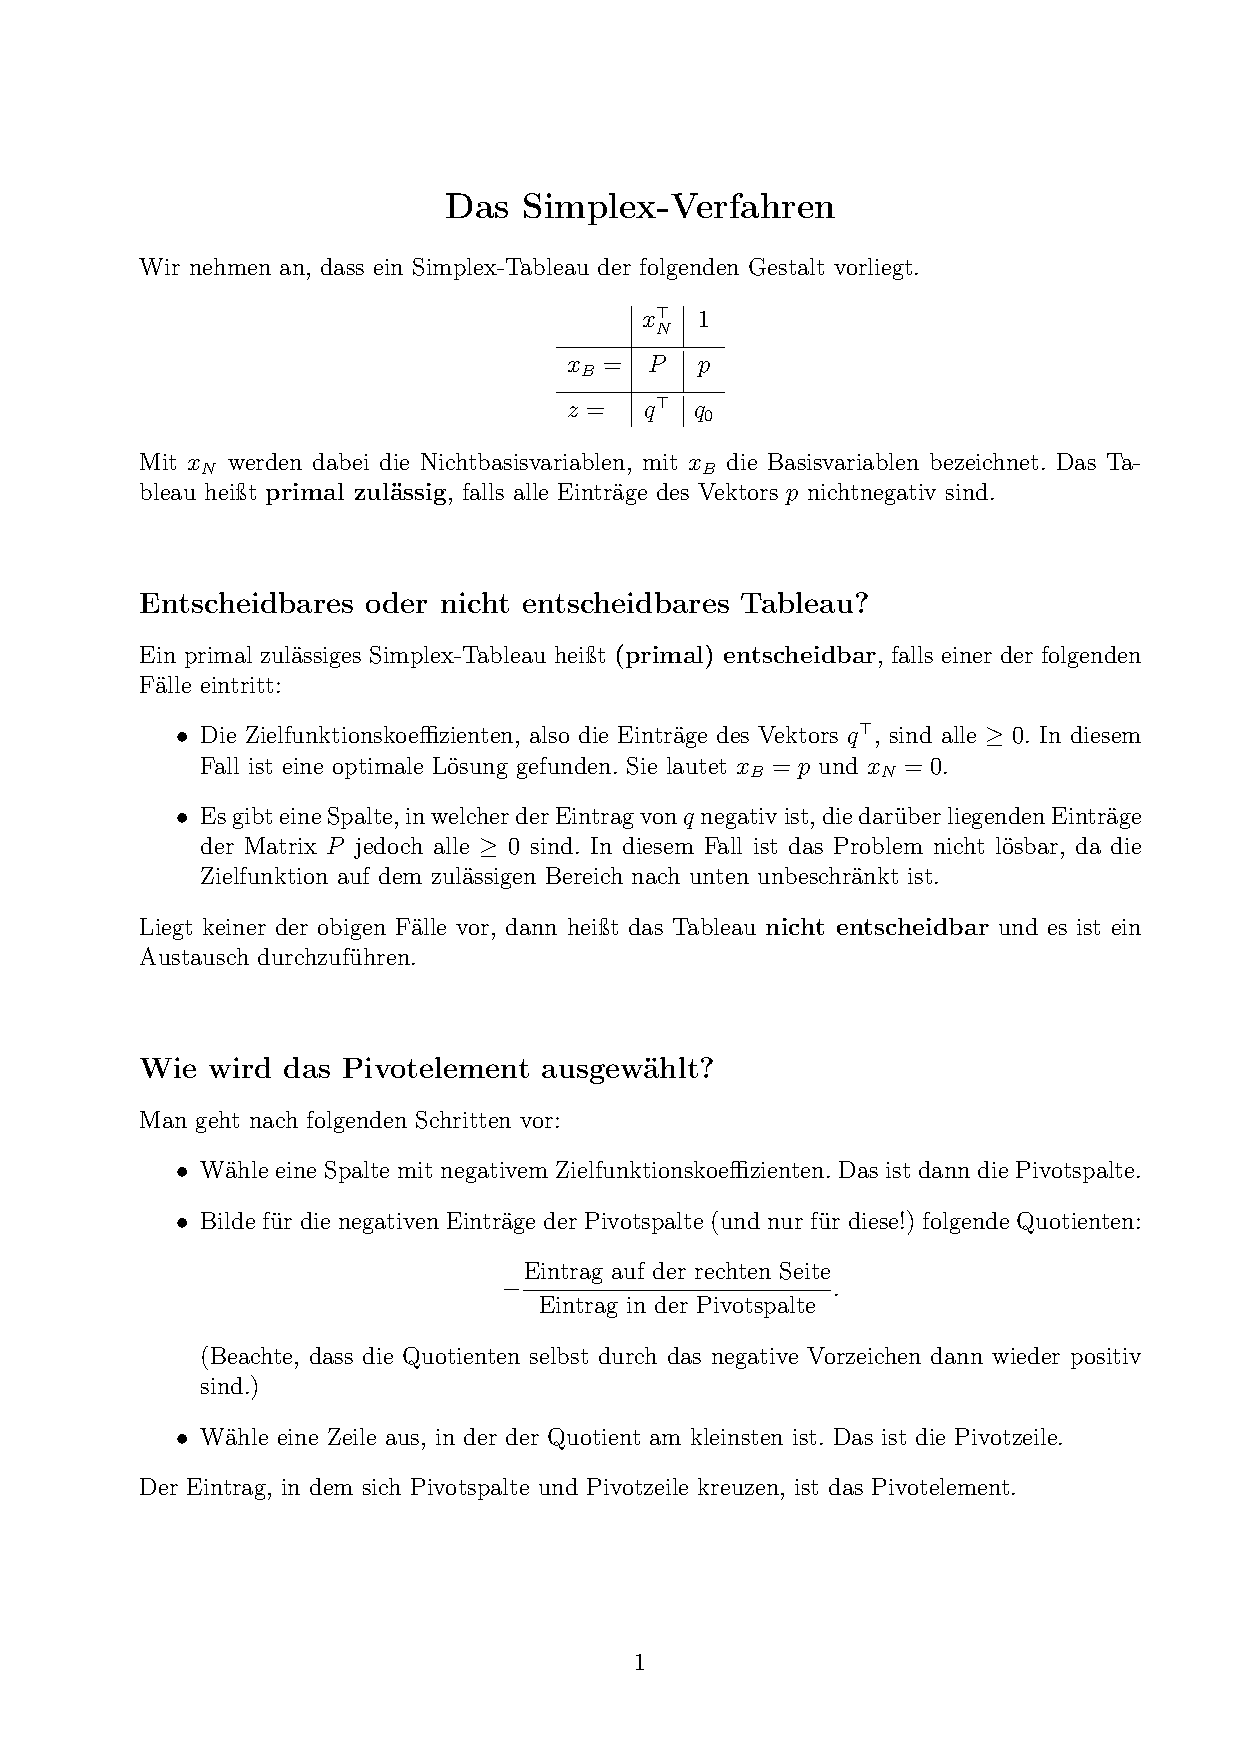
\includepdf[pages=-]{optinum_zsfSimplex.pdf}

\begin{beispiel} %3.3
	Wir betrachten wie in \cref{beispiel: 3.2} die Optimierungsaufgabe
	\begin{equation*}
	z = -x_1 - x_2 \to \min \quad \bei \quad x_1 + 2 x_2 \le 6, \enskip 4x_1 + x_2 \le 10, \enskip x_1, x_2 \ge 0
	\end{equation*} 
	mit Simplex-Starttableau:
	\begin{indentpar}
		\begin{tabular}{R{1.8cm}|R{0.6cm}R{0.6cm}|R{0.6cm} l}
			$T_0$ & $x_1$ & $x_2$ & $1$ \\ \cline{1-4}
			$x_3 = $ & $-1$ & $\fbox{-2}$ & $6$ & {\footnotesize $\quer{t} = 3$} \\ 
			$x_4 = $ & $-4$ & $-1$ & $10$ & {\footnotesize $\quer{t} = 10$} \\ \cline{1-4}
			$z =$ & $-1$ & $-1$    & $0$ \\ \cline{1-4}
			Kellerzeile & $-\frac{1}{2}$ & $\ast$ & $3$ & {\footnotesize = neue Pivotzeile}
		\end{tabular}
	\end{indentpar}
	Nun wählen wir aber $\tau = 2$, woraus sich $\sigma =  3$ ergibt.
	Zur besseren Übersicht haben wir eine Kellerzeile eingeführt. Diese entspricht genau der neu berechneten Pivotzeile.
	\begin{indentpar}
		\begin{tabular}{R{1.8cm}|R{0.6cm}R{0.6cm}|R{0.6cm} l}
			$T_1$ & $x_1$ & \textcolor{cdpurple}{$x_3$} & $1$ \\ \cline{1-4}
			\textcolor{cdpurple}{$x_2 = $} & $- \sfrac{1}{2}$ & $-\sfrac{1}{2}$ & $3$ & {\footnotesize (Division durch -1 * Pivot)} \\ 
			$x_4 = $ & $-\sfrac{7}{2}$ & $\sfrac{1}{2}$ & $7$ \\ \cline{1-4}
			$z =$ & $-\sfrac{1}{2}$ & $\sfrac{1}{2}$  & $-3$ \\ \cline{1-4}
			Kellerzeile & $-\sfrac{2}{7}$ & $\sfrac{1}{7}$ & $2$
		\end{tabular}
	\end{indentpar}
	Nebenrechnung: z.B. $ 7 = 10 + 3 * (-1)$
	
	Im nächsten Schritt wählen wir nun $\tau = 1$ und $\sigma = 4$.
	\begin{indentpar}
		\begin{tabular}{R{1.8cm}|R{0.6cm}R{0.6cm}|R{0.6cm} l}
			$T_2$ & \textcolor{cdpurple}{$x_4$} & $x_3$ & $1$ \\ \hline
			$x_2 = $ & $\sfrac{1}{7}$ & $-\sfrac{4}{7}$ & $2$ & \\ 
			\textcolor{cdpurple}{$x_1 = $} & $-\sfrac{2}{7}$ & $\sfrac{1}{7}$ & $2$ \\ \hline
			$z =$ & $\sfrac{1}{7}$ & $\sfrac{3}{7}$  & $-4$ 
		\end{tabular}
	\end{indentpar}
	Da $\schlange{p} = \brackets{\begin{smallmatrix} 2 \\ 2 \end{smallmatrix}} \ge 0$ ist, ist die Lösung zulässig. Außerdem wissen wir wegen $\trans{\schlange{q}} = \brackets{\sfrac{1}{7}, \sfrac{3}{7}} \ge 0$, dass die Lösung optimal ist. Somit ergibt sich
	\begin{equation*}
		x^\ast = (x_1^\ast, x_2^\ast, x_3^\ast, x_4^\ast) = (2,2,0,0) \mit z^\ast = -4
	\end{equation*}
\end{beispiel}

\subsection{Phase 1 (Hilfsfunktionsmethode)}

Wir betrachten das Problem
\begin{equation}
	z = \trans{c} x \to \min \bei Ax = b , x \ge 0
	\label{eq: 3.7}
\end{equation}
Ohne Einschränkung sei $b \ge 0$. Durch folgendes Hilfsproblem lässt sich eine Startecke ermitteln (sofern eine solche überhaupt existiert). 
\begin{equation}
	h = \trans{e} y \to \min \bei y + Ax = b, x \in \Rn_+, y \in \Rm_+
	\label{eq: 3.8}
\end{equation}
mit $e = \transpose{1, \dots , 1} \in \Rm$.
Eine erste Basislösung für \eqref{eq: 3.8} ist gegeben durch 
\begin{equation}
	\begin{array}{@{}r|c|c@{}}
		T_0 & x & 1 \\ \hline
		y =  & -A & b \\ \hline
		h = & -\trans{e}A & \trans{e} b
	\end{array}
	\label{eq: 3.9}
\end{equation}

\begin{satz} %3.8
	Das Problem \eqref{eq: 3.7} besitzt genau dann eine zulässige Lösung, wenn $h_{\min} = 0$ den Optimalwert von \eqref{eq: 3.8} darstellt.
\end{satz}
\begin{proof}
	Offenbar gilt $h_{\min} = 0 \equivalent y = 0$.
	\begin{proof-equivalence}
		\hinrichtung Besitzt \eqref{eq: 3.7} eine zulässige Lösung $\schlange{x}$, dann ist $\left( \begin{smallmatrix} \schlange{x} \\ 0 \end{smallmatrix} \right)$ zulässig für \eqref{eq: 3.8}. Wegen $0 \le h = \trans{e} \schlange{y} = 0$ folgt $h_{\min} = 0$.
		\rueckrichtung Hat man umgekehrt $h_{\min} = 0$, so gilt $\schlange{y} = 0$ für jede optimale Lösung $\left( \begin{smallmatrix} \schlange{x} \\ \schlange{y} \end{smallmatrix} \right)$ von \eqref{eq: 3.8}. Aus der Zulässigkeit von $\left( \begin{smallmatrix} \schlange{x} \\ \schlange{y} \end{smallmatrix} \right)$ für \eqref{eq: 3.8} folgt dann die Zulässigkeit von $\schlange{x}$ für \eqref{eq: 3.7}.
	\end{proof-equivalence}
\end{proof}

\subsection{Der Simplexalgorithmus}

Mit den zuvor beschriebenen Vorgehensweisen lässt sich das Simplexverfahren zur Lösung der Optimierungsaufgabe \eqref{eq: 3.1} wie folgt algorithmisch formulieren:
\begin{itemize}
	\item \textbf{Schritt 1} (\textit{Initialisierung}): Ermittle eine erste zulässige Basislösung $x = \transpose{\trans{x_B}, \trans{x_N}} = \transpose{\trans{p}, \trans{0}}$ mit $p = (A_B)^{-1} b \ge 0$, wobei $I_B$ die Menge der Basisindizes ist und stelle ein erstes Simplextableau auf.
	\item \textbf{Schritt 2} (\textit{Optimalitätstest}): Berechne entsprechend \cref{aussage: 3.4}
	\begin{equation}
		\quer{q} \defeq \min_{j \in I_N} q_j \quad \mit \quad q_J \defeq c_j \trans{d} A^j \enskip (j \in I_N)
		\label{eq: 3.10}
	\end{equation}
	wobei $\trans{d} \defeq \trans{c_B} (A_B)^{-1}$ ist. Gilt $\quer{q} \ge 0$, dann ist $x$ Lösung von \eqref{eq: 3.1}. Andernfalls sei $q_\tau = \quer{q} < 0$.
	\item \textbf{Schritt 3} (\textit{Test auf Unbeschränktheit}): Gilt $P_{i \tau} \ge 0$ für alle $I \in I_B$, so ist die Aufgabe nicht lösbar ($f^\ast = -\infty$).
	\item \textbf{Schritt 4} (\textit{Austauschschritt}): Bestimme die Pivotzeile $\sigma$ gemäß
	\begin{equation*}
		- \frac{p_\sigma}{P_{\sigma \tau}} = \min \menge{- \frac{p_i}{P_{i \tau}} \colon \quer{P}_{i \tau} < 0, i \in I_B}
	\end{equation*}
	und führe den Austauschschritt $\sigma \leftrightarrow \tau$ (Aktualisierung Simplextableau) durch. Gehe zu Schritt 2.
\end{itemize}

\begin{bemerkung} %3.3
	\begin{enumerate}[label=(\roman*), nolistsep, topsep=-\parskip]
		\item Der Simplexalgorithmus löst Problem \eqref{eq: 3.1} nach endlich vielen Schritten exakt oder stellt dessen Unlösbarkeit fest.
		\item Pro Simplexschritt ist im Wesentlichen die Matrix $P$ (der Dimension $m \times (n-m)$ ) zu transformieren. Für $n \gg m$ kann das recht aufwendig sein, sodass ggf. alternative Varianten des Simplexalgorithmus' (z.B. das revidierte Simplexverfahren oder die Technik der Spaltengenerierung) effizienter sind.
		\item Der Test auf Unbeschränktheit der Zielfunktion kann auch für jede Spalte $j \in I_N$ mit $q_j < 0$ erfolgen, sofern dies nicht zu aufwendig ist.
	\end{enumerate}
\end{bemerkung}
\section{Das duale Simplexverfahren}

Nach \cref{aussage: 3.4} ist ein Tableau
\begin{center}
	\begin{tabular}{r|c|c}
		$T_0$ & $x_N$ & $1$ \\ \hline
		$x_B = $ & $P$ & $p$ \\ \hline
		$z =$ & $\trans{q}$ & $q_0$
	\end{tabular}
\end{center}
optimal, wenn $p \ge 0$ und $q \ge 0$ gelten. Nach Konstruktion gilt beim primalen Simplexverfahren stets $p \ge 0$.
Sei nun ein Tableau $T_0$ gegeben mit $q \ge 0$, aber \textit{nicht} $p \ge 0$, d.h. es gibt eine Zeile $\sigma \in I_B$ mit $p_\sigma < 0$.
Die zu $T_0$ gehörige Basislösung ist dann \textit{nicht} zulässig. Mithilfe des dualen Simplexverfahrens lässt sich jedoch (unter Beibehaltung von $q \ge 0$) eine zulässige Basislösung (d.h. mit $p \ge 0$) erzeugen.
Entsprechend der bekannten Austauschregeln ergeben sich folgende Bedingungen:
\begin{equation*}
	\begin{alignedat}{2}
		\schlange{q}_j &\defeq q_j - \frac{P_{\sigma, j}}{P_{\sigma, \tau}} q_\tau &\overset{!}&{\ge} 0 \qquad \forall j \in I_N \setminus \menge{\tau} \\
		\schlange{q}_\tau &\defeq \frac{q_\tau}{P_{\sigma, \tau}} &\overset{!}&{\ge} 0  \\
		\schlange{p}_\sigma &\defeq - \frac{p_\sigma}{P_{\sigma, \tau}} &\overset{!}&{\ge} 0
	\end{alignedat}
\end{equation*}
Wegen $p_\sigma < 0$ und $q_\tau \ge 0$ ist somit ein Pivotelement mit $P_{\sigma, \tau} > 0$ zu wählen. Zur Sicherstellung von $\schlange{q}_j \ge 0$ für alle $j \in I_N \setminus \menge{\tau}$ muss ferner gelten
\begin{equation*}
	\frac{q_\tau}{P_{\sigma, \tau}} = \min \menge{\frac{q_j}{P_{\sigma, j}} \colon P_{\sigma, j} > 0, j \in I_N}
\end{equation*}
Die eigentlichen Austauschregeln sind analog zu denen des primalen Simplexverfahrens.

\begin{bemerkung} %3.4
	Da dieses Verfahren mit einem \textit{unzulässigen} Punkt startet, ist die Folge der Zielfunktionswerte (im Gegensatz zum primalen Simplexverfahren) nicht monoton fallend.
\end{bemerkung}

\begin{bemerkung} %3.5
	Falls eine zulässige Basislösung gefunden wird, so ist diese zwangsläufig optimal.
\end{bemerkung}

\begin{beispiel}
	Betrachten wir die Optimierungsaufgabe
	\begin{equation*}
		\begin{aligned}
			z = 6x_1 + 5x_2 + 12x_3 + 8x_4 + 9x_5 \to \min \quad \bei \quad 
			x_1 + x_3 + x_4 + x_5 &\ge 300, \\
			x_2 + 2x_3 + x_4 &\ge 400, \\
			x_i &\ge 0 \qquad \forall i = 1, \dots, 5
		\end{aligned}
	\end{equation*}
	Um daraus Gleichungsrestriktionen zu machen, führen wir Schlupfvariablen $x_6, x_7 \ge 0$ ein, d.h.
	\begin{equation*}
		\begin{aligned}
			x_1 + x_3 + x_4 + x_5 &= 300 + x_6 , \\
			x_2 + 2x_3 + x_4 &= 400 + x_7, \\
			x_i &\ge 0 \qquad \qquad \forall i = 1, \dots, 7
		\end{aligned}
	\end{equation*}
	Daraus ergibt sich nun folgendes Tableau
	\begin{indentpar}
		\begin{tabular}{R{1cm}|R{.5cm}R{.5cm}R{.5cm}R{.5cm}R{.5cm}|R{.9cm}l}
			$T_0$ & $x_1$ & $x_2$ & $x_3$ & $x_4$ & $x_5$ & $1$ \\ \cline{1-7}
			$x_6 =$ & $1$ & $0$ & $1$ & $1$ & $1$ & $-300$ \\
			$x_7 =$ & $0$ & \fbox{$1$} & $2$ & $1$ & $0$ & $-400$ & $\leftarrow \sigma = 7$ \\ \cline{1-7}
			$z =$   & $6$ & $5$ & $12$ & $8$ & $9$ & $0$ \\ \cline{1-7}
			Keller  & $0$ & $\ast$ & $-2$ & $-1$ & $0$ & $400$
		\end{tabular}
	\end{indentpar}
	
	Zur Wahl von $\tau = 2$: $\frac{5}{1}$, $\frac{12}{2} = 6$, $\frac{8}{1} = 8$. Dabei ist $5$ minimal, also $\tau = 2$.
	Fahren wir nun mit den weiteren Tableaus fort:
	
	\begin{indentpar}
		\begin{tabular}{R{1cm}|R{.5cm}R{.5cm}R{.5cm}R{.5cm}R{.5cm}|R{.9cm}l}
			$T_1$   & $x_1$ & $x_7$  & $x_3$      & $x_4$ & $x_5$ & $1$ \\ \cline{1-7}
			$x_6 =$ & $1$   & $0$    & \fbox{$1$} & $1$   & $1$   & $-300$ & $\leftarrow \sigma = 6$ \\
			$x_2 =$ & $0$   & $1$    & $-2$       & $-1$  & $0$   & $400$ \\ \cline{1-7}
			$z =$   & $6$   & $5$    & $2$        & $3$   & $9$   & $2000$ \\ \cline{1-7}
			Keller  & $0$   & $\ast$ & $\ast$ & $-1$  & $0$   & $400$
		\end{tabular}

		\begin{tabular}{R{1cm}|R{.5cm}R{.5cm}R{.5cm}R{.5cm}R{.5cm}|R{.9cm}l}
			$T_2$   & $x_1$ & $x_7$ & $x_6$ & $x_4$      & $x_5$ & $1$ \\ \cline{1-7}
			$x_3 =$ & $1$   & $0$   & $1$   & $-1$       & $1$   & $300$  \\
			$x_2 =$ & $2$   & $1$   & $-2$  & \fbox{$1$} & $2$   & $-200$ & $\leftarrow \sigma = 2$ \\ \cline{1-7}
			$z =$   & $4$   & $5$   & $2$   & $1$        & $7$   & $2600$ \\ \cline{1-7}
			Keller  & $-2$  & $-1$  & $2$   & $\tau = 4$ & $-2$  & $200$
		\end{tabular}
	
		\begin{tabular}{R{1cm}|R{.5cm}R{.5cm}R{.5cm}R{.5cm}R{.5cm}|R{.9cm}l}
			$T_3$   & $x_1$ & $x_7$ & $x_6$ & $x_2$ & $x_5$ & $1$ \\ \cline{1-7}
			$x_3 =$ & $1$   & $1$   & $-1$   & $-1$  & $1$   & $100$  \\
			$x_4 =$ & $-2$   & $-1$   & $2$  & $1$   & $-2$   & $200$ \\ \cline{1-7}
			$z =$   & $2$   & $4$   & $4$   & $1$   & $5$   & $2800$ \\
		\end{tabular}
	\end{indentpar}

	Somit ergibt sich die Lösung
	\begin{equation*}
		x^\ast = \transpose{0,0,100,200,0,0,0} \quad \und \quad z^\ast = 2800
	\end{equation*}
\end{beispiel}
\section{Dualität}

Wir betrachten nun die Optimierungsaufgabe
\begin{equation*}
	\begin{aligned}
		\qquad &\trans{c} x \to \min \bei Ax \le b \und x \in \Rn_+ \\
		&I \defeq \menge{1, \dots, m} \und J \defeq \menge{1, \dots, n}
	\end{aligned} \tag{P}
	% \label{eq: 3.11}
	\label{eq: P}
\end{equation*}

\begin{satz}[Charakterisierungssatz] %3.9
	\label{satz: 3.9}
	Ein Punkt $x \in \Rn$ ist genau dann Lösung von (P), wenn ein $\quer{x} \in \Rm$ existiert, sodass insgesamt das folgende System gelöst wird:
	\begin{equation*}
		\begin{alignedat}{3}
			A \quer{x} - b &\le 0 \quad &\quer{x} &\ge 0 \qquad \qquad &(1) \\
			\trans{A} \quer{u} + c &\ge 0 \quad &\quer{u} &\ge 0 &(2) \\
			\trans{\quer{u}} \brackets{A \quer{x} - b} &= 0 \qquad \qquad &\trans{\quer{x}} \brackets{\trans{A}\quer{u} + c} &= 0 &(3)
		\end{alignedat}
	\end{equation*}
\end{satz}
\begin{proof}
	Die vorliegende Optimierungsaufgabe ist äquivalent zu
	\begin{equation*}
		f(x) = \trans{c} x \to \min \bei \underbrace{\begin{pmatrix} A \\ - \one_n \end{pmatrix}}_{= \schlange{A} \in \R^{(m + n) \times n}} x \le \underbrace{\begin{pmatrix} b \\ 0 \end{pmatrix}}_{= \schlange{b} \in \R^{m+n}}
		\tag{P'}
		\label{eq: P'}
	\end{equation*}
	Gemäß \cref{lemma: 2.8} ist $x$ genau dann Lösung von \eqref{eq: P'} (und \eqref{eq: P}), wenn ein Vektor $w = \left( \begin{smallmatrix} u \\ v \end{smallmatrix} \right) \in \R^{m + n}$ existiert mit 
	\begin{equation*}
		\begin{alignedat}{2}
			\nabla f(x) + \sum_{i \in I \cup J} w_i \schlange{a}_i &= 0 \\
			w_i &\ge 0 \qquad \qquad &&(i \in I \cup J) \\
			\trans{\schlange{a}_i} x - \schlange{b}_i &\le 0 &&(i \in I \cup J) \\
			w_i \brackets{\trans{\schlange{a}_i} x - b_i} &= 0 &&(i \in I \cup J)
		\end{alignedat}
		\tag{KKT}
	\end{equation*}
	Trennung von $I$ und $J$ führt zu
	\begin{equation*}
		c + \sum_{i \in I} u_i a_i + \sum_{j \in J} v_j (-e^j) = 0
		\tag{KKT}
	\end{equation*}
	\begin{equation*}
		\begin{alignedat}{4}
			u_i &\ge 0 \qquad &&(i \in I) 											& v_j &\ge 0 \qquad &&(j \in J) \\
			\trans{a_i} x - b_i &\le 0 &&(i \in I) 									& \transpose{-e^j} x - 0 &\le 0 &&(j \in J) \\
			u_i \brackets{\trans{a_i} x - b_i} &= 0 &&(i \in I) \qquad\quad	& v_j \brackets{\transpose{-e^j} x - 0} &= 0 &&(j \in J)  \\
		\end{alignedat}
	\end{equation*}
	Überführt man dieses System in eine Matrix-Vektor-Schreibweise, so ergibt sich
	\begin{equation*}
		\begin{aligned}
			c + \trans{A} u - v &= 0 \\
			u,v,x &\ge 0 \\
			Ax - b &\le 0 \\
			\trans{u} \brackets{Ax - b} &= 0 \\
			\trans{x} v &= 0
		\end{aligned}
	\end{equation*}
	Durch Umstellen der ersten Gleichung nach $v$ lässt sich diese Variable im System ''eliminieren`` und wir erhalten die Behauptung.
\end{proof}

\begin{definition} %3.3
	Das Problem
	\begin{equation}
		\text{(D)} \qquad z_D = -\trans{b} u \to \max \quad \bei \quad \trans{A} u \ge -c, \enskip u \in \R_+^m 
		\label{eq: 3.12}
	\end{equation}
	heißt duale Optimierungsaufgabe zu (P).
\end{definition}

\textbf{Begründung:} Die Anwendung von \cref{satz: 3.9} auf (D) ergibt das selbe KKT-System wie im Falle von (P). Dazu müssen wir (D) umformulieren als Minimierungsaufgabe
\begin{equation*}
	- z_D = \trans{b} u \to \min \quad \bei \quad -\trans{A} u \le c, \enskip u \in \R_+^m
\end{equation*}
(damit die selbe Form wie in \cref{satz: 3.9} vorliegt).
Einsetzen in (1) - (3) ergibt
\begin{equation*}
	\begin{alignedat}{3}
		\text{(1)} &\leadsto &-\trans{A} u - c &\le 0, \enskip &u &\ge 0 \\
		\text{(2)} &\leadsto &\transpose{-\trans{A}} y + b &\ge 0, \enskip &y &\ge 0 \\
		\text{(3)} &\leadsto \quad &\trans{y} \brackets{-\trans{A} u - c} &= 0, \quad &\trans{u} \brackets{\transpose{-\trans{A}} y + b} &= 0
	\end{alignedat}
\end{equation*}
Umformulierung liefert
\begin{equation*}
	\begin{alignedat}{4}
		\text{(1)} &\leadsto &\trans{A} u +  c &\ge 0, \enskip &u &\ge 0 \qquad &&\text{entspricht (2) aus System für (P)} \\
		\text{(2)} &\leadsto &Ay - b &\le 0, &y &\ge 0 \qquad &&\text{entspricht (1) aus System für (P) mit $y = x$} \\
		\text{(3)} &\leadsto \quad &\trans{y} \brackets{\trans{A} u + c} &= 0, \quad &\trans{u} \brackets{Ay - b} &= 0 \qquad &&\text{entspricht (3) aus System für (P)}
	\end{alignedat}
\end{equation*}
(D) liefert also dasselbe System (1) - (3) wie (P).

\begin{satz}[schwache Dualität] %3.10
	Sei $x$ zulässig für (P) und $u$ zulässig für (D). Dann gilt
	\begin{equation*}
		-\trans{b} u \le \trans{c} x
	\end{equation*}
\end{satz}
\begin{proof}
	Es gilt
	\begin{align*}
		-\trans{b} u &\le \transpose{-Ax} u = - \trans{x} \trans{A} u \tag{$Ax \le b, u \ge 0$} \\
		&\le \trans{x} c = \trans{c} x \tag{$\trans{A} u \ge -c, x \ge 0$}
	\end{align*}
\end{proof}

\begin{satz}[starke Dualität] %3.11
	Die Optimierungsaufgabe (P) ist genau dann lösbar, wenn (D) lösbar ist. Für die zugehörigen Lösungen $\quer{x}$ und $\quer{u}$ gilt dann
	\begin{equation*}
		- \trans{b} \quer{u} = \trans{c} \quer{x}
	\end{equation*}
	also die Gleichheit der Optimalwerte.
\end{satz}
\begin{proof}
	Der erste Teil der Aussage folgt direkt aus der Gleichheit der KKT-Systeme. Aus Eigenschaft (3) des KKT-Systems folgt dann die Gleichheit der Optimalwerte mittels
	\begin{equation*}
		\trans{\quer{u}} \brackets{A \quer{x} - b} = 0 = \trans{\quer{x}} \brackets{\trans{A} \quer{u} + c} \follows - \trans{b} \quer{u} = \trans{\quer{u}} A \quer{x} = \trans{c} \quer{x}
	\end{equation*}
\end{proof}

Aus dem schwachen Dualitätssatz folgt insbesondere auch, dass die Existenz eines dual (primal) zulässigen Punktes eine endliche untere (obere) Schranke für den primalen (dualen) Optimalwert liefert.

\begin{folgerung} %3.12
	\begin{equation*}
		\text{(P) lösbar } \equivalent \text{ (D) lösbar } \equivalent \exists \ x \ge 0, u \ge 0 \colon Ax \le b, \trans{A} u \ge -c
	\end{equation*}
\end{folgerung}

Die Bedingungen (3) im KKT-System werden \begriff{Komplementaritätsbedingungen} genannt.

zum Beispiel: $\trans{u} \brackets{Ax - b} = 0, x \ge 0, u \ge 0,  Ax - b \le 0$, d.h. $u_i (Ax - b)_i = 0$ für alle $i$.

Es ist möglich, primale und duale Aufgabe gleichzeitig innerhalb eines Tableaus zu lösen:
\begin{equation*}
	\begin{alignedat}{4}
		(P) \quad &z_P &=   \trans{c} x \to \min \quad  &\bei \quad          A x &\le b, &x &\ge 0 \\
		(D) \quad &z_D &= - \trans{b} u \to \max \quad &\bei \quad - \trans{A} u &\le c, &u &\ge 0
	\end{alignedat}
\end{equation*}
Durch Einführen von Schlupfvariablen $s \ge 0$, $v \ge0$ erhält man
\begin{equation*}
	\begin{alignedat}{5}
		(P) \quad &   z_P &= \trans{c} x \to \min \quad &\bei \quad &s &= b - Ax, &x &\ge 0, &s &\ge 0 \\
		(D) \quad & - z_D &= \trans{b} u \to \min \quad &\bei \quad &v &= c + \trans{A} u, &u &\ge 0, &v &\ge 0
	\end{alignedat}
\end{equation*}

\begin{center}
	\begin{tabular}{r|c|c}
		$T_0$ & $x$ & $1$ \\ \hline
		$s = $ & $-A$ & $b$ \\ \hline
		$z_P =$ & $\trans{c}$ & $0$
	\end{tabular}
    $\quad$ bzw. $\quad$
	\begin{tabular}{r|c|c}
		$T_0$ & $u$ & $1$ \\ \hline
		$v = $ & $\trans{A}$ & $c$ \\ \hline
		$- z_D =$ & $\trans{b}$ & $0$
	\end{tabular}
\end{center}

Beide Schemata sind (gewissermaßen) zueinander transponiert.
Das duale Simplexverfahren für (P) kann als primales Simplexverfahrens für (D) interpretiert werden.
\section{Transportoptimierung}

\subsection{Problemstellung}

\textbf{Zur Erinnerung:}
Es gebe Erzeuger $i \in I = \menge{0, \dots, r}$ und Verbraucher $k \in K = \menge{1, \dots, s}$. Weiterhin seien die Kosten $c_{ik}$ für den Transport einer Einheit von $i$ nach $k$ sowie der Vorrat $a_i > 0$ und der Bedarf $b_k > 0$ für alle $i \in I$ und $k \in K$ bekannt. Wie ist der gesamte Transport kostenminimal zu gestalten.

Als Variablen verwenden wir die Transportmenge $x_{ik}$ von $i$ nach $k$.
\begin{equation}
\begin{alignedat}{3}
	z = \sum_{i \in I} \sum_{k \in K} c_{ik} x_{ik} \to \min \quad \bei \quad 
	&\sum_{k \in K} x_{ik} &= a_i \quad &(i \in I) \\
	&\sum_{i \in I} x_{ik} &= b_k \quad &(k \in K) \\
	& x_{ik} &\ge 0 \quad &(i,k) \in I \times K \\
\end{alignedat}
\label{eq: 3.13}
\end{equation}

Mit   
\begin{equation*}
	\begin{aligned}
		x &= \transpose{x_{11}, x_{12}, \dots, x_{1s}, x_{21}, \dots, x_{rs}} \\
		c &= \transpose{c_{11}, c_{12}, \dots, c_{1s}, c_{21}, \dots, c_{rs}} \\
		\quer{b} &= \transpose{a_1, \dots, a_r, b_1, \dots, b_s}
	\end{aligned}
\end{equation*}
hat \eqref{eq: 3.13} die Form
\begin{equation*}
	z = \trans{c} x \to \min \bei Ax = \quer{b}, x \ge 0
\end{equation*}

\begin{bemerkung} %3.6
	Das Transportproblem ist eine sehr spezielle Optimierungsaufgabe. Die Koeffizientenmatrix 
	\begin{equation*}
		A = 
		\left( \begin{array}{cccc|cccc|cccc}
		1 & 1 & \cdots & 1 &   &   &        &   &   &   &        &\\
		  &   &        &   & 1 & 1 & \cdots & 1 &   &   &        &\\
		  &   &        &   &   &   &        &   & 1 & 1 & \cdots & 1  \\
		\hline
		1 &   &        &   & 1 &   &        &   & 1 &   &        &  \\
		  & \multicolumn{2}{c}{\ddots} & & & \multicolumn{2}{c}{\ddots} & & & \multicolumn{2}{c}{\ddots} & \\
		  &   &        & 1 &   &   &        & 1 &   &   &        & 1  \\	  
		\end{array} \right) \in \R^{(r+s) \times (r*s)}
	\end{equation*}
	ist schwach besetzt. Insbesondere hat die Spalte von $A$, die zur Variablen $x_{ik}$ gehört, die Gestalt $A^{ik} = \begin{psmallmatrix} e^i \\ e^k \end{psmallmatrix} \in \R^{r+s}$.
\end{bemerkung}

\begin{satz} %3.13
	Das Transportproblem ist genau dann lösbar, wenn die Sättigungsbedingung
	\begin{equation}
		\sum_{i \in I} a_i = \sum_{k \in K} b_k
		\label{eq: 3.15}
	\end{equation}
	gilt.
\end{satz}
\begin{proof}
	Wir zeigen zuerst, dass \eqref{eq: 3.15}  äquivalent zu $G \neq \emptyset$ ist.
	\begin{itemize}
		\item Einerseits folgt aus $x \in G \neq \emptyset$ durch Summation der Gleichungsnebenbedingungen
		\begin{equation*}
			\sum_{i \in I} a_i = \sum_{i \in I} \sum_{k \in K} x_{ik} = \sum_{k \in K} \sum_{i \in I} x_{ik} = \sum_{k \in K} b_k
		\end{equation*}
		\item  Gilt hingegen \eqref{eq: 3.15}, so ist mit $\sigma \defeq \sum_{i \in I} a_i = \sum_{k \in K} b_k$ ein zulässiger Punkt $x = (x_{ik})$ wie folgt definiert:
		\begin{equation*}
			x_{ik} \defeq \frac{a_i b_k}{\sigma}
		\end{equation*}
	\end{itemize}
	Der zulässige Bereich $G$ ist polyedrisch (und damit abgeschlossen) und ferner wegen $0 \le x_{ik} \le \min\menge{a_i, b_k}$ beschränkt und somit kompakt.
	Mit dem Satz von Weierstraß\footnote{Die Zielfunktion ist linear, d.h. stetig, auf einer komapkten Menge $G$.} folgt dann die Lösbarkeit des Transportproblems.
\end{proof}

Die Systemmatrix $A$ besitzt für praxisrelevante Problemgrößen eine sehr große Anzahl an Einträgen, sodass die Anwendung des Simplexverfahrens im Allgemeinen nicht empfehlenswert ist; insbesondere deshalb, weil dieses die Struktur von $A$ nicht mit einbezieht.

Zur Lösung des Transportproblems hat sich daher ein Verfahren etabliert, das auch die duale Aufgabe 
\begin{equation}
	w \defeq \trans{a} u + \trans{b} v \to \max \bei \trans{A} \begin{psmallmatrix} u \\ v \end{psmallmatrix} \le c, u \in \R^r, v \in \R^s
	\label{eq: 3.16}
\end{equation}
bzw.
\begin{equation}
	w \defeq \sum_{i \in I} a_i u_i + \sum_{k \in K} b_k v_k \to \max \bei u_i + v_k \le c_{ik} \quad (u_i, v_k \in \R, i \in I, k \in K)
	\label{eq: 3.17}
\end{equation}
löst.

\begin{satz}[Optimalitätskriterium] %3.14
	\label{satz: 3.14}
	Sei $x \in G$, d.h. $x$ ist zulässiger Transportplan, dann gilt
	\begin{equation*}
		\begin{aligned}
			x \text{ optimal} \equivalent \exists u \in \R^r, v \in \R^s \mit u_i + v_k \le c_{ik}, x_{ik} * (c_{ik} - u_i - v_k) = 0 \quad \forall i \in I, k \in K
		\end{aligned}
	\end{equation*}
\end{satz}
\begin{proof}
	Nach dem Charakterisierungssatz gilt: $x \in G$ ist genau dann optimal, wenn duale Variablen $u \in \R^r$ und $v \in \R^s$ existieren, sodass $(u,v)$ dual zulässig ist und die Komplementaritätsbedingungen gelten.
\end{proof}

\begin{aussage} %3.15
	Der Rang von $A$ ist $\card{I} + \card{K} - 1 = r+s-1$.
\end{aussage}
\begin{proof}
	Einerseits sind die Spalten $A^{11}, \dots, A^{1s}, A^{21}, A^{31}, \dots, A^{r1}$ von $A$ linear unabhängig, d.h. $\rg(A) \ge r + s - 1$.
	Andererseits ist die Summe der ersten $r$ Zeilen identisch mit der Summe der letzten $s$ Zeilen. Somit ist der Rang von oben beschränkt mit $\rg(A) \le r + s -1$.
\end{proof}

\begin{folgerung} %3.16
	Jede Ecke des zulässigen Bereichs $G$ hat höchstens $r+s-1$ positive Komponenten.
\end{folgerung}

\begin{definition} %3.4
	Eine Folge von Zellen (Indexpaaren) $(i_1, k_1)$, $(i_2, k_1)$, $(i_2, k_2)$ $\dots$ $(i_\ell, k_\ell)$, $(i_1, k_\ell)$, $(i_1, k_1)$ mit $i_\nu \neq i_\mu$ und $k_\nu \neq k_\mu$ für $\nu \neq \mu$ heißt \begriff{Zyklus} (der Länge $2 \ell$).
\end{definition}

\begin{beispiel} %3.5
	Im folgenden Schema ist ein Zyklus der Länge $2 \ell = 8$ abgebildet:
	\begin{center}
		\begin{tabular}{l|ccccc}
			$i / k$ & 1 & 2 & 3 & 4 & 5 \\ \hline
			1       & $\ast$ & & $\ast$ & & \\
			2 & & $\ast$ & & & $\ast$ \\
			3 & $\ast$ & & & & $\ast$ \\
			4 & & $\ast$ & $\ast$ & & 
		\end{tabular}
	\end{center}
	Dieses Beispiel spielt eine wichtige Rolle bei der Feststellung, ob ein gegebener Transportplan eine Ecke von $G$ ist.
\end{beispiel}

\begin{aussage} %3.17
	\begin{enumerate}[label=(\roman*), nolistsep, topsep=-\parskip]
		\item Sei $J$ eine Menge von Zellen. Gilt $\card{J} \ge r+s$, so enthält $J$ mindestens einen Zyklus.
		\item Sei $x = (x_{ik})$ ein zulässiger Transportplan. $x$ ist genau dann eine Ecke von $G$, wenn $J_+ \defeq \menge{(i,k) : x_{ik} > 0}$ keinen Zyklus enthält.
	\end{enumerate}
\end{aussage}
\begin{proof}
	vielleicht in der Übung --- oder auch nicht.
\end{proof}

\subsection{Erzeugung eines ersten Transportplans}
Dieser Teil entspricht der ersten Phase des Simplexverfahrens, d.h. also der Bestimmung einer Startecke.
Gemäß der vorherigen Beobachtungen genügt es einen zyklenfreien zulässigen Transportplan zu finden. Hierfür können unterschiedliche Methoden genutzt werden.

\begin{description}
	\item[Nordwest-Ecken-Regel:] Die jeweilige noch nicht belegte Nordwest-Zelle wird mit maximaler Transportmenge belegt.
	\item[Regel der minimalen Kosten:] In jedem Schritt wird eine noch nicht belegte Zelle, die minimale Kosten hat, mit maximaler Transportmenge belegt.
	\item[Methode von Vogel:] Bestimme in jeder Zeile und Spalte die Differenz der zwei kleinsten Kostenkoeffizienten der noch freien Zellen. Wähle dann eine Zeile/Spalte mit maximaler Differenz und belege die Zelle mit kleinsten Kosten.
\end{description}

Darstellung der Inputdaten oder zulässigen Punkte in folgenden Schemata:

\begin{minipage}{\dimexpr0.5\linewidth-\fboxrule-\fboxsep}
	\centering
	\begin{tabular}{c|cccc}
		C & $b_1$ & $b_2$ & $\dots$ & $b_s$ \\ \hline
		$a_1$ & $c_{11}$ & $c_{12}$ & $\dots$ & $c_{1s}$ \\
		$\vdots$  & $\vdots$ & $\vdots$ & $\ddots$ & $\vdots$ \\
		$a_r$ & $c_{r1}$ & $c_{r2}$ & $\dots$ & $c_{rs}$
	\end{tabular}
	\captionof{table}{Inputdaten}
\end{minipage}
\begin{minipage}{\dimexpr0.5\linewidth-\fboxrule-\fboxsep}
	\centering
	\begin{tabular}{c|cccc}
		X & $b_1$ & $b_2$ & $\dots$ & $b_s$ \\ \hline
		$a_1$ & $x_{11}$ & $x_{12}$ & $\dots$ & $x_{1s}$ \\
		$\vdots$  & $\vdots$ & $\vdots$ & $\ddots$ & $\vdots$ \\
		$a_r$ & $x_{r1}$ & $x_{r2}$ & $\dots$ & $x_{rs}$
	\end{tabular}
	\captionof{table}{Transportplan}
\end{minipage}




\begin{beispiel} %3.6
	\label{beispie: 3.6}
	Gegeben Sei das folgende Transportproblem:
	\begin{center}
		\begin{tabular}{r|rrrrr}
			C & 12 &  5 &  6 &  7 &  7 \\ \hline
			4 & 12 &  6 & 10 &  9 &  5 \\
			19 & 10 & 16 & 17 &  3 &  7 \\
			14 &  4 & 11 &  5 &  8 & 10
		\end{tabular}
	\end{center}
	
	Man erhält folgende Startecken:
	\begin{center}
		\begin{tabular}{r|rrrrr}
			$\text{X}_{\text{NW}}$ & \cancel{12} \cancel{8} 0 &  \cancel{5} 0 &  \cancel{6} 0 &  \cancel{7} 0 &  \cancel{7} 9 \\ \hline
			0 &  4 &  0 &  0 &  0 &  0 \\
			0 \cancel{6} \cancel{11} \cancel{19} &  8 & 5 & 6 & 0 & 0 \\
			0 \cancel{7} \cancel{14} &  0 & 0 &  0 &  7 & 7
		\end{tabular}
	\end{center}

	Zielfunktionswert: $z(x_{\text{NW}}) = 4 * 12 + 8 * 10 + 5 * 16 + 6 * 17 + 7 * 8 + 7 * 10 = 436$
	
	\vspace{\parskip}
	
	\begin{center}
		\begin{tabular}{r|rrrrr}
			$\text{X}_{\text{MK}}$ & 12 &  5 &  6 & \cancel{7} 0 &  \cancel{7} 3 \\ \hline
			0 \cancel{4} & 0 &  0 & 0 &  0 &  $\fbox{4}^3$ \\
			0 \cancel{12} \cancel{19} & 0 & $\fbox{5}$ & $\fbox{4}$ &  $\fbox{7}^1$ &  $\fbox{3}$ \\
			0 \cancel{2} \cancel{14} &  $\fbox{12}^2$ & 0 &  $\fbox{2}^4$ &  0 & 0
		\end{tabular}
	\end{center}

	Zielfunktionswert: $z(x_{\text{MK}}) = 268$

	\vspace{\parskip}
	
	\begin{center}
		\begin{tabular}{r|rrrrr}
			$\text{X}_{\text{V}}$ & 12 &  5 &  6 &  7 &  7 \\ \hline
			4 &  &  4 &  &   &   \\
			19 &  & 1 & 4 &  7 &  7 \\
			14 &  12 &  &  2 &   & 
		\end{tabular}
	\end{center}
	Zielfunktionswert: $z(x_{\text{V}}) = 236$
\end{beispiel}

Je nach Qualität der Startlösung können unterschiedlich viele Iterationen des Transportalgorithmus vonnöten sein.

\subsection{Der Transportalgorithmus}

Ausgehend von einer Startlösung berechnet der Algorithmus zunächst ein Paar $(u,v)$ dualer Variablen und prüft dann die Optimalität mit \cref{satz: 3.14}. Liegt keine Optimalität vor, wird ein neuer Plan erzeugt.

\textbf{Vorgehensweise:}

\begin{enumerate}
	\item Bestimme einen zulässigen, zyklenfreien Transportplan $X_0$ mit genau $r+s-1$ markierten Basiszellen. (Diese bilden dann die Menge $J_B = J_B(X_0)$.)
	\item Bestimme für den aktuellen Plan $X$ die zugehörigen dualen Variablen $u_i$ und $v_k$ aus dem Gleichungssystem 
	\begin{equation}
		u_i + v_k = c_{ik} \qquad (i,k) \in J_B = J_B(X)
		\label{eq: 3.18}
	\end{equation}
	\item Berechne für alle $(i,k) \notin J_B$ die Koeffizienten $w_{ik} = c_{ik} - u_i - v_k$. Falls $w_{ik} \ge 0$ für alle Zellen ist, dann ist $X$ optimal. Andernfalls wähle man eine Zelle $(p,q)$ mit $w_{pq} = \min\menge{w_{ik} : i \in I, k \in K} < 0$.
	\item Markiere $(p,q)$ im Schema von $X$, bestimme den  (eindeutigen) Zyklus $J_{pq}$ in $J_B \cup \menge{(p,q)}$ und markiere abwechselnd die Zellen in $J_{pq}$ mit ''+`` und ''-``. Sei $J_{pq}^-$ die Menge der mit ''-`` gekennzeichneten Zellen.
	\item Ermittle $\delta = x_{gh} \defeq \min\menge{x_{ik} : (i,k) \in J_{pq}^-}$ und aktualisiere den Plan $X$ gemäß
	\begin{equation*}
		X^{\text{neu}} \defeq \brackets{x_{ik}^{\text{neu}}} \quad \mit \quad  
		x_{ik}^{\text{neu}} \defeq \begin{cases}
		x_{ik} + \delta & \text{ falls }(i,k) \in \brackets{J_{pq} \cup \menge{(g,h)}} \setminus J_{pq}^-\\
		x_{ik} - \delta & \text{ falls }(i,k) \in J_{pq}^-\\
		x_{ik} & \text{ sonst}
		\end{cases}
	\end{equation*}
	Aktualisiere die Menge der Basiszellen
	\begin{equation*}
		J_B^{\text{neu}} \defeq \brackets{J_B \cup \menge{(p,q)}} \setminus \menge{(g,h)}
	\end{equation*}
	und gehe zu Schritt 2.
\end{enumerate}

\begin{bemerkung} %3.7
	Aufgrund von $\card{J_B} = r + s - 1$ ist das in Schritt 2 zu lösende Gleichungssystem (zur Ermittlung von $u$ und $v$) unterbestimmt. Eine der Variablen kann also beliebig festgelegt werden. Die in Schritt 3 bestimmten Werte $w_{ik}$ sind jedoch unabhängig von dieser Wahl.
\end{bemerkung}

Im gesamten Algorithmus gilt stets $w_{ik} = 0$ für die aktuellen Basiszellen $(i,k) \in J_B$ (per Konstruktion in Schritt 2), diese beeinflussen den Optimalitätstest in Schritt 3 also nicht. Daher kann zur Darstellung das folgende komprimierte Schema genutzt werden:

\begin{center}
	\begin{tabular}{c|cccc}
		T & $v_1$ & $v_2$ & $\dots$ & $v_s$ \\ \hline
		$u_1$ & \fbox{$x_{11}$} & $w_{12}$  & $\dots$ & $w_{1s}$ \\
		$u_2$ & $w_{21}$ & $w_{22}$ & \fbox{$x_{23}$} & $w_{2s}$ \\
		$\vdots$ &  $\vdots$ & $\vdots$ & $\vdots$ & $\vdots$ \\
		$u_r$ & $w_{r1}$ & \fbox{$x_{r2}$} & $\dots$ & $w_{rs}$ 
	\end{tabular}
\end{center}


\begin{beispiel}[Fortsetzung von \cref{beispie: 3.6}] %3.7
	Gegeben Sei das Problem
	\begin{center}
		\begin{tabular}{r|rrrrr}
			C & 12 &  5 &  6 &  7 &  7 \\ \hline
			4 & 12 &  6 & 10 &  9 &  5 \\
			19 & 10 & 16 & 17 &  3 &  7 \\
			14 &  4 & 11 &  5 &  8 & 10
		\end{tabular}
	\end{center}
	Mit der Minimale-Kosten-Regel haben wir bereits den Plan $X_0$ bestimmt:
	\begin{center}
		\begin{tabular}{r|rrrrr}
			$X_0$ & 12 &  5 &  6 & 7 & 7 \\ \hline
			4 & 0 &  0 & 0 &  0 &  \fbox{4} \\
			19 & 0 & \fbox{5} & \fbox{4} &  \fbox{7} &  \fbox{3} \\
			14 &  \fbox{12} & 0 &  \fbox{2} &  0 & 0
		\end{tabular}
	\end{center}
	Bestimmung der dualen Variablen (Potenziale) $u_i$ und $v_k$
	\begin{center}
		\begin{tabular}{l|ccccc}
			$T_0$ & $v_1=16$ & $v_2 = 16$ & $v_3=17$ & $v_4=3$ & $v_5=7$ \\ \hline
			$u_1 = -2$ & $-2$ & $-8$  & $-5$ & $8$ & \fbox{$4$} \\
			$u_2 = 0$ & $-6$ & \fcolorbox{black}{cdgray!10}{$5$} & \fbox{$4$} &\fbox{$7$} & \fbox{$3$} \\
			$u_3 = \fcolorbox{cdgreen!10}{cdgreen!10}{-12}$ &  \fbox{$12$} & $7$ & \fbox{$2$} & $17$ & $15$ \\
		\end{tabular}
	\end{center}
	\fcolorbox{black}{cdgray!10}{$5$} : $\underbrace{u_2}_{=0} + v_2 = c_{22} = 16 \follows v_2 = 16$
	
	\fcolorbox{cdgreen!10}{cdgreen!10}{$-12$} : $u_3 + \underbrace{v_3}_{=17} = c_{33} = 5 \follows u_3 = c_{33} - 17 = -12$
	
	Dieser Plan ist nicht optimal, da negative Einträge $w_{ik}$ existieren.
	Wir wählen also den eindeutig bestimmten Zyklus $-8 \to 4 \to 3 \to 5 \to 8$ und geben alternierende ''Vorzeichen``, d.h. $-8^+ \to 4^- \to 3^+ \to 5^- \to 8^+$. 	
	Wir wählen das kleinste mit einem ''$-$`` markierte Zellenelement des Zyklus: $\delta = \min\menge{x_{ik} : (i,k) \in J_{pq}^-} = 4$.
	
	Ein neuer Plan ergibt sich nun mit
	\begin{center}
		\begin{tabular}{l|ccccc}
			$X_1$ & \\ \hline
			&  & \fcolorbox{black}{cdgray!10}{$4$}  & & & $0$ \\
			&  & \fbox{$1$} & \fbox{$4$} &\fbox{$7$} & \fbox{$7$} \\
			&  \fbox{$12$} &  & \fbox{$2$} & &  \\
		\end{tabular}
	\end{center}

	Achtung: $x_{21} = \fcolorbox{black}{cdgray!10}{4}$ war vorher nicht in der Basis (also $x_{21} = 0$) und somit $x_{21}^{\text{neu}} = x_{21} + \delta = 4$.
	
	Bestimmung der Potenziale $u_i$ und $v_k$ für $X_1$:
	\begin{center}
		\begin{tabular}{l|ccccc}
			$T_1$ & $v_1=16$ & $v_2 = 16$ & $v_3=17$ & $v_4=3$ & $v_5=7$ \\ \hline
			$u_1 = -10$ & $6$ & \fbox{$4$}  & $4$ & $16$ & $8$ \\
			$u_2 = 0$ & $-6$ & \fbox{$1$} & \fbox{$4$} &\fbox{$7$} & \fbox{$7$} \\
			$u_3 = -12$ &  \fbox{$12$} & $7$ & \fbox{$2$} & $17$ & $15$ \\
		\end{tabular}
	\end{center}
	Auch dieses Tableau ist noch nicht optimal. Wir erkennen den Zyklus $-6^+ \to 12^- \to 2^+ \to 4^-$.
	
	Ein neuer Plan ergibt sich zu
	\begin{center}
		\begin{tabular}{l|ccccc}
			$X_2$ & \\ \hline
			&  & \fbox{$4$}  & & &  \\
			& \fbox{$4$} & \fbox{$1$} & &\fbox{$7$} & \fbox{$7$} \\
			&  \fbox{$8$} &  & \fbox{$6$} & &  \\
		\end{tabular}
	\end{center}
	mit den Potenzialen
	\begin{center}
		\begin{tabular}{l|ccccc}
			$T_2$ & $v_1=10$ & $v_2 = 16$ & $v_3=11$ & $v_4=3$ & $v_5=7$ \\ \hline
			$u_1 = -10$ & $12$ & \fbox{$4$}  & $9$ & $16$ & $8$ \\
			$u_2 = 0$ & \fbox{$4$} & \fbox{$1$} & $6$ &\fbox{$7$} & \fbox{$7$} \\
			$u_3 = -6$ & \fbox{$8$} & $1$ & \fbox{$6$} & $11$ & $9$ \\
		\end{tabular}
	\end{center}

	Alle $w_{ik} \ge 0$, d.h. der das Tableau ist optimal und $X_2$ ist eine Lösung der gegebenen Optimierungsaufgabe. Es gilt $z(X_2) = 212$.
\end{beispiel}

\chapter{Diskrete Optimierung}
\label{chapter_4_diskreteOptimierung}
In diesem Kapitel befassen wir uns mit Techniken zur Lösung ganzzahliger Optimierungsaufgaben. Dabei dürfen einige oder gar alle Variablen diskrete Werte annehmen.
Somit entfällt eine Argumentation über Ableitung, zulässige Richtungen etc. Ganzzahlige Optimierungsaufgaben sind also \enquote{schwieriger} als die zugehörige stetige Relaxation. Dennoch kann, in einigen Fällen, das Lösen diskreter Aufgaben auch zur effizienten Lösung stetiger Aufgaben beitragen, wie folgendes Beispiel verdeutlicht.
\section{Spaltengenerierung}

Wir betrachten die stetige Relaxation des Bin-Packing-Problems (vgl. \cref{subsec: 1.3.2}). Zur Erinnerung: Es sind $b_i$ Teile der Länge $\ell_i$ ($i = 1, \dots, m$) in möglichst wenige Behälter der Kapazität $L$ zu packen. 
\begin{itemize}[nolistsep, topsep=-\parskip]
	\item Packungsvarianten: $a^j = \transpose{a_1^j , \dots , a_m^j} \in \Z_+^m$ mit $\trans{\ell}a^j \le L$ ($j \in J$)
	\item Variablen: $x_j$ beschreibt Häufigkeit, wie oft Variante $a^j$ genutzt wird.
\end{itemize}
\begin{equation*}
	z = \sum_{j \in  J} x_j \to \min \quad \bei \quad \sum_{j \in J} a_i^j * x_j = b_i \quad (i \in I) \quad \und \quad x_j \ge 0 \quad (j \in J)
\end{equation*}
Grundsätzlich ist diese Aufgabe mit dem Simplexverfahren lösbar, jedoch gibt es im Allgemeinen exponentiell viele Variablen, sodass pro Austauschschritt ein großer Aufwand entstünde.

Wir können uns hierbei zu Nutze machen, dass alle Spalten der Systemmatrix $A$ eine gemeinsame Struktur aufweisen:
\begin{equation*}
	a^j \text{ ist Spalte von } A \equivalent a^j \in \Z_+^m \und \trans{\ell} a^j \le L
\end{equation*}

Offenbar gilt hier $c = e = \transpose{1, \dots, 1}$, sodass für eine gewählte Basismatrix $A_B$ in Schritt 2 des Simplexalgorithmus folgendes zu bestimmen wäre:
\begin{equation*}
	\quer{q} \defeq \min_{j \in J_N} q_j \quad \mit \quad q_j = c_j - \trans{d} a^j = 1 - \trans{d}a^j, \quad a^j \in \Z_+^m, \trans{\ell} a^j \le L
\end{equation*}
wobei $\trans{d} \defeq \trans{c_B} A_B^{-1}$. In Schritt 2 wäre folglich die Aufgabe 
\begin{equation*}
	1 - \trans{d} a^j = q_j \to \min \bei \trans{\ell} a^j \le L \und a^j \in \Z_+^m
\end{equation*}
bzw. 
\begin{equation*}
	\trans{d} a^j \to \max \bei \trans{\ell} a^j \le L, a^j \in \Z_+^m
\end{equation*}
zu lösen.
Gilt $q_j^\ast < 0$, so liegt keine Optimalität vor und eine zugehörige Lösung $a^{j, \ast}$ wäre in die Basismatrix aufzunehmen. Gilt $g_j^\ast \ge 0$, so sind wir fertig.
\section{Die Methode Branch \& Bound}

Branch \& Bound (B\&B) ist eine sehr flexible Technik, um exakte Lösungsverfahren für Probleme der diskreten Optimierung zu entwickeln. Anschaulich betrachtet wird dabei eine schwierige Optimierungsaufgabe sukzessiv in Teilprobleme zerlegt, die wiederum \enquote{leicht} (näherungsweise) gelöst werden können und somit zur Lösung des Gesamtproblems beitragen. Näherungslösungen erhält man dabei oftmals mithilfe geeigneter Relaxationen.

\subsection{Grundlagen}

Wir betrachten das Anfangsproblem
\begin{equation*}
	f(x) \to \min \bei x \in E \cap D
	\tag{$P_0$}
	\label{eq: p_0}
\end{equation*}
und eine zugehörige Relaxation
\begin{equation*}
	g(x) \to \min \bei x \in E
	\tag{Q}
	\label{eq: q}
\end{equation*}
wobei $g(x) \le f(x)$ auf $D \cap E$ gilt.

\vspace{\parskip}
\fbox{\textbf{Prinzip der B\&B-Methode}}

Die Menge $E$ wird durch Separation in Teilmengen $E_i$ mit $i \in I$ zerlegt. Dadurch entstehen \begriff{Teilprobleme} 
\begin{equation*}
	f(x) \to \min \bei x \in D \cap E_i
	\tag{$P_i$}
	\label{eq: p_i}
\end{equation*}
Jedem dieser Teilprobleme \eqref{eq: p_i} soll nun eine Zahl $b(P_i)$, genannt \begriff{untere Schranke}, zugeordnet werden, sodass gilt
\begin{enumerate}[label=(\alph*), nolistsep]
	\item $b(P_i) \le \min\menge{f(x) : x \in D \cap E_i}$
	\item $b(P_i) = f(\dach{x})$ falls $D \cap E = \menge{\dach{x}}$
	\item $b(P_i) \le b(P_j)$ falls $E_j \subset E_i$
\end{enumerate}

Eine geeignete Möglichkeit besteht darin, z.B. die stetige Relaxation der Teilprobleme \eqref{eq: p_i} zu betrachten, d.h. 
\begin{equation*}
	b(P_i) \defeq \begin{cases}
	\min\menge{g(x) : x \in E_i} & \falls \card{E_i \cap D} > 1 \\
	f(\dach{x}) & \falls \card{E_i \cap D} = 1 \\
	+ \infty & \falls E_i \cap D = \emptyset
	\end{cases}
\end{equation*}

\pagebreak

\subsection{Allgemeiner B\&B-Algorithmus}
Bezeichne mit $R$ die Menge der noch zu bearbeitenden Teilprobleme (''Restmenge``) und mit $\quer{z}$ den Zielfunktionswert der bisher besten gefundenen zulässigen Lösung $\quer{x} \in D \cap E$.

\begin{enumerate}[label=\underline{\textbf{Schritt \arabic*:}}, leftmargin=*]
	\setcounter{enumi}{-1}
	\item \textbf{Initialisierung} --- Bestimme $b(P_0)$.
	\begin{enumerate}[label=(\alph*), noitemsep]
		\item Falls $\quer{x} \in D \cap E$ bekannt ist mit $f(\quer{x}) = b(P_0)$, dann \texttt{STOP}.
		\item Setze $R \defeq \menge{P_0}$ und $\quer{z} \defeq + \infty$ oder $\quer{z} = f(x)$, wenn ein $x \in D \cap E$ bekannt ist.
	\end{enumerate}	
	\item \textbf{Abbruchtest} --- Falls $R \neq \emptyset$, dann \texttt{STOP}. Falls $\quer{z} = +\infty$, dann ist \eqref{eq: p_0} nicht lösbar (leerer zulässiger Bereich), andernfalls ist $\quer{x}$ Lösung von \eqref{eq: p_0}
	\item \textbf{Strategie} --- Wähle entsprechend einer Auswahlstrategie ein $P_i \in R$ und setze $R \defeq R \setminus \menge{P_i}$.
	\item \textbf{Zerlegung (''branch``)} --- Zerlege $P_i$ durch Separation in endlich viele Teilprobleme $P_{i,1}, \dots, P_{i,k_i}$. Setze $j \defeq 1$.
	\item \textbf{Schranken- und Dominanztests (''bound``)}
	\begin{enumerate}[label=(\alph*), noitemsep]
		\item Berechne $b(P_{i,j})$. Falls dabei ein $\schlange{x} \in D \cap E$ gefunden wurde mit $f(\schlange{x}) < \quer{z}$, setze $\quer{x} \defeq \schlange{x}$ und $\quer{z} \defeq f(\schlange{x})$.
		\item Falls $b(P_{i,j}) < \quer{z}$, dann setze $R \defeq R \cup \menge{P_{i,j}}$. Falls $j < k_i$, setze $j \defeq j + 1$ und gehe zu (a).
		\item Setzte $R \defeq R \setminus \menge{P_k}$ für alle $P_k \in R$ mit $b(P_k) \ge \quer{z}$. 
	\end{enumerate}	
	Gehe zu Schritt 1.
\end{enumerate}

\begin{*bemerkung}
	\begin{enumerate}
		\item Die Endlichkeit des Verfahrens ist zu sichern, z.B. durch $\card{E_{i,j} \cap D} \le \card{E_i \cap D}$ für alle $j$ (falls $E_i \cap D$ endlich ist) oder durch $b(P_{i,j}) > b(P_i) + \epsilon$ mit $\epsilon > 0$ für alle $j$ und $i$.
		\item Das B\&B-Verfahren kann mithilfe eines Verzweigungsbaumes veranschaulicht werden.
		\item In Schritt 2 können verschiedene Auswahlstrategien gewählt werden, z.B. 
		\begin{itemize}[noitemsep]
			\item \begriff{Minimalsuche} (best bound search): wähle $P_i \in R$ mit $b(P_i) \le b(P_k)$ für alle $P_k \in R$.
			\item \begriff{Tiefensuche} (depth-first search, LIFO): wähle $P_i \in R$ mit kleinstem Schrankenwert unter allen Teilproblemen mit maximaler Verzweigungstiefe.
			\item \begriff{Breitensuche} (breadth-first-search, FIFO): wähle $P_i \in R$ mit kleinstem Schrankenwert unter allen Teilproblemen mit minimaler Verzweigungstiefe.
		\end{itemize}
	\end{enumerate}
\end{*bemerkung}

\subsection{Beispiele für B\&B-Verfahren}

\subsubsection{Das 0/1-Rucksackproblem}

Zur Erinnerung: Gegeben seien ganze Zahlen $c_i > 0$, $0 < a_i < b$ für $i \in I \defeq \menge{1, \dots, n}$
\begin{align*}
	f(x) &= \trans{c} x \to \max \bei \trans{a} x \le b, \enskip x \in \menge{0,1}^n 
	\tag{P} \\
	f(x) &= \trans{c} x \to \max \bei \trans{a} x \le b, \enskip x \in [0,1]^n 
	\tag{Q} \label{eq: rucksack-q}
\end{align*}
Hier gilt also $E = \menge{x \in \Rn : \trans{a} x \le b, 0 \le x \le 1, i \in I}$ und $D = \mathbb{B}^n = \menge{0,1}^n$.

\begin{bemerkung}
	Die stetige Relaxation \eqref{eq: rucksack-q} besitzt unter der Voraussetzung
	\begin{equation*}
		\frac{c_i}{a_i} \ge \frac{c_{i+1}}{a_{i+1}} \quad \text{ für } 1 \le i \le n
	\end{equation*}
	die Lösung
	\begin{equation*}
		\dach{x_i} = 1 \quad (i = 1, \dots, k) \qquad \dach{x}_{k+1} = \frac{b - \sum_{i=1}^k a_i}{a_{k+1}} \qquad \dach{x}_i = 0 \enskip i = k+2, \dots, n 
		\tag{R} \label{eq: rucksack-r}
	\end{equation*}
	mit $k \defeq \max\menge{j \in I : \sum_{i=1}^j a_i \le b}$.
\end{bemerkung}

\begin{*bemerkung_inline}
	Wir sortieren also abfallend nach Nutzen pro Volumen und packen dann soviel wie möglich in den Rucksack ($k$ Elemente). Dann füllen wir den Restplatz noch mit (einem Anteil von) dem nächsten Element auf ($k+1$-tes Element), alles danach können wir nicht mehr mitnehmen.
\end{*bemerkung_inline}

Innerhalb des Verzweigungsbaums ergeben sich die folgenden Teilprobleme (für bereits fixierte Variablen $\quer{x}_i$, $i \in I_k \subseteq I$).
\begin{align*}
	\sum_{i \in I_k} c_i \quer{x}_i + \sum_{i \notin I_k} c_i x_i &\to \max \bei \sum_{i \notin I_k} a_i x_i \le b - \sum_{i \in I_k} a_i \quer{x}_i, \quad i \notin I_k, x_i \in \mathbb{B}
	\tag{$P_k(\quer{x})$} \label{eq: rucksack-pk}\\
	\sum_{i \in I_k} c_i \quer{x}_i + \sum_{i \notin I_k} c_i x_i &\to \max \bei \sum_{i \notin I_k} a_i x_i \le b - \sum_{i \in I_k} a_i \quer{x}_i, \quad i \notin I_k, x_i \in [0,1]  \tag{$Q_k(\quer{x})$} \label{eq: rucksack-qk}
\end{align*}

\textbf{Beachte:} Da es sich um eine Maximierungsaufgabe handelt, werden im B\&B-Algorithmus \textit{obere} Schranken $b(P_k(\quer{x}))$ benötigt. Diese gewinnen wir aus den Optimalwerten der stetigen Relaxation $Q_k(\quer{x})$.

\begin{beispiel}
	Gegeben sei das binäre Rucksackproblem 
	\begin{equation*}
	\begin{split}
	\setlength{\arraycolsep}{2pt}
	\begin{array}{rcrcrcrcrcrcrcrl}
	z = \trans{c} x &= &8x_1 &+ &16x_2 &+ &20x_3 &+ &12x_4 &+ &6x_5 &+ &10x_6 &+ &4x_7 &\to \max \\
	\bei \trans{a} x &= &3x_1 &+ &7x_2 &+ &9x_3 &+ &6x_4 &+ &3x_5 &+ &5x_6 &+ &2x_7 &\le 17 = b, 
	\end{array}
	\\
	x_i \in \menge{0,1}, i = 1, \dots, 7
	\end{split}
	\tag{P} \label{eq: rucksack-bsp-p}
	\end{equation*}
	
	\begin{itemize}[leftmargin=*]
		\item Die korrekte Sortierung liegt bereits vor.
		\item Wurzelknoten \eqref{eq: rucksack-bsp-p}$=(\text{P}_0)$: Die stetige Relaxation besitzt die Lösung $x_1 = x_2 = 1$ und $x_3 = \frac{7}{9}$ sowie $x_4 = \dots = x_7 = 0$. Somit ist $b(\text{P}_0) = \lfloor 8 + 16 + 20 * \frac{7}{9} \rfloor = 39$. Die Abrundung ist dabei erlaubt, da $\trans{c} x \in \Z$ für alle zulässigen Punkte von \eqref{eq: rucksack-bsp-p}. Ein zulässiger Punkt für \eqref{eq: rucksack-bsp-p} ist gegeben durch $\quer{x}_1 = \quer{x}_2 = \quer{x}_4 = 1$, $\quer{x}_i = 0$ sonst. Dabei ist $z(\quer{x}) = 8 + 16 + 12 = 36 \defqe \quer{z}$. Wegen $36 < 39$ muss weiter verzweigt werden.
		\item Verzweigung: $x_3 = 0$ vs. $x_3 = 1$.
		\begin{itemize}
			\item Teilproblem: $(P_1) = (P_{0,1})$. Setzt man $x_3 = 0$, so hat die stetige Relaxation die Lösung $x_1 = x_2 = x_4 = 1$, $x_5 = \frac{1}{3}$ und $x_6 = x_7 = 0$. Somit ist $b(P_1) = \lfloor 8 + 16 + 12 + 6 * \frac{1}{3} \rfloor = 38$. Ein daraus ableitbarer Punkt ist gegeben durch $\quer{x}_1 = \quer{x}_2 = \quer{x}_4 = 1$ mit $z = 36$, d.h. $\quer{z}$ muss nicht aktualisiert werden.
			\item $(P_2) = (P_{0,2})$. Setzt man $x_3 = 1$, so erhält man $x_1 = 1$, $x_2 = \frac{5}{7}$ mit $b = \lfloor 8 + 20 + 16 * \frac{5}{7} \rfloor = 39$ und einen zulässigen Punkt für \eqref{eq: rucksack-bsp-p} durch $\quer{x}_1 = \quer{x}_3 = \quer{x}_5 = \quer{x}_7 = 1$ mit $\quer{z} = 38$, d.h. $\quer{z}$ wurde verbessert.
			\item Damit kann ($P_1$) abgeschlossen werden, da maximal noch der Zielfunktionswert $38$ möglich ist, der in ($P_2$) bereits erreicht worden ist.
		\end{itemize}
		%
		\item Verzweigung: $x_2 = 0$ vs. $x_2 = 1$.
		\begin{itemize}
			\item Teilproblem $(P_3) = (P_{2,1})$. Setzt man $x_2 = 0$ (und $x_3 = 1$ von oben), dann hat die stetige Relaxation die Lösung $x_1 = 1$, $x_4 = \frac{5}{6}$ mit $b(P_3) = 38 = \quer{z}$, also sind wir hier fertig.
			\item Teilproblem $(P_4) = (P_{2,2})$. Setzt man $x_2 = 1$ (und $x_3 = 1$) so folgt $x_1 = \frac{1}{3}$, also $b(P_4) = 38 = \quer{z}$, d.h. wir sind hier wieder fertig.
		\end{itemize}
		%
		\item Nun ist $R = \emptyset$ und wir haben eine Lösung gefunden:
		\begin{equation*}
			x_1 = x_3 = x_5 = x_7 = 1 \quad \mit \quad z = 38
		\end{equation*}
	\end{itemize}
\end{beispiel}


%%%%%%%%%%%%%%%%%%%%%%%%%%%%%%%%%%%%%%%%%%%%%%%%%%%%%%%%%%%%%%%%%%%%%%%%%%%%%%%%%%
%%%%%%%%%%%%%%%%%%%%%%%%%%%%%%%%%%%%%%%%%%%%%%%%%%%%%%%%%%%%%%%%%%%%%%%%%%%%%%%%%%


\subsubsection{Ganzzahlige lineare Optimierung nach Land/Doig/Dahin}

Wir betrachten die ganzzahlige Optimierungsaufgabe 
\begin{equation*}
	\trans{c}x  \to \min \bei x \in D \cap E
	\tag{P} \label{eq: ldl-p}
\end{equation*}
mit $D = \Z^n$ und $E = E_0 = \menge{x \in \Rn: Ax = b, x \ge 0}$, wobei alle Inputdaten $(A,b,c)$ ganzzahlig sind. Die im Verlauf des Verfahrens zu betrachtenden Teilprobleme \eqref{eq: ldl-pi} haben die Form
\begin{equation*}
	\trans{c} x \to \min \bei x \in D \cap E_i
	\tag{P${}_\text{i}$} \label{eq: ldl-pi}
\end{equation*}
wobei $E_i$ durch eine oder mehrere zusätzliche Ungleichungen aus $E_0$ entsteht. Sei $x^{\text{LP}}$ eine Lösung der zu \eqref{eq: ldl-pi} gehörenden stetigen Relaxation
\begin{equation*}
	z(Q_i) = \min \menge{\trans{c} x : x \in E_i} 
	\tag{Q${}_\text{i}$} \label{eq: ldl-qi}
\end{equation*}
mit $x^{\text{LP}}_j \notin \Z$ für mindestens einen Index $j$. Dann kann der (gerundete) Optimalwert als Schranke $b(P_i)$ genutzt werden.
\begin{align*}
	E_{i,1} &= \menge{x \in E_i : x_j \le \left\lfloor x^{\text{LP}} \right\rfloor}
	\tag{P${}_{i,1}$} \\
	E_{i,2} &= \menge{x \in E_i : x_j \ge \left\lfloor x^{\text{LP}} \right\rfloor + 1 = \left\lceil x^{\text{LP}} \right\rceil} 
	\tag{P${}_{i,2}$}	
\end{align*}

\begin{bemerkung}
	Das Runden des Optimalwertes einer Relaxation zur Schrankenbestimmung ist nur für $c \in \Z^n$ zulässig.
\end{bemerkung}

\begin{beispiel}
	Betrachte 
	\begin{equation*}
	\begin{alignedat}{4}
		z = -7x_1 - 2x_2 \to \min \bei &&-x_1 &+ &2x_2 &+ &x_4 &= 4 \\
		&&5x_1 &+ &x_2 &+ &x_4 &= 20, \quad x_1, \dots, x_n \in \Z_+
	\end{alignedat}
	\end{equation*}
	Die Relaxation ergibt sich durch $x_1, \dots, x_n \ge 0$.
	\begin{itemize}[leftmargin=*]
		\item Wurzelknoten:
		\begin{center}
			\begin{tabular}{r|rr|r}
				$T_1$ & $x_1$ & $x_2$ & $1$ \\ \hline
				$x_3 = $ & $1$ & $-2$ & $4$ \\
				$x_4 = $ & $-5$ & $-1$ & $20$ \\ \hline
				$z = $   & $-7$ & $-2$ & $0$
			\end{tabular}
			$\qquad \overset{x_1 \leftrightarrow x_4}{\longrightarrow} \quad \dots \quad \overset{x_2 \leftrightarrow x_3}{\longrightarrow} \qquad$
			\begin{tabular}{r|rr|r}
				$T_3$ & $x_4$ & $x_3$ & $1$ \\ \hline
				$x_2 = $ & $-\frac{1}{11}$ & $-\frac{5}{11}$ & $\frac{40}{11}$ \\
				$x_1 = $ & $\frac{-2}{11}$ & $\frac{1}{11}$ & $\frac{36}{11}$ \\ \hline
				$z = $   & $\frac{16}{11}$ & $\frac{3}{11}$ & $-\frac{332}{11}$
			\end{tabular}
		\end{center}	
		%
		\item Verzweigung: nach $x_2$, da $\min \menge{4-\frac{40}{11}, \frac{40}{11} - 3} > \min \menge{4 - \frac{36}{11}, \frac{36}{11} - 3}$. 
		\begin{itemize}
			\item 1. Teilproblem: $x_2 \ge 4$ (führe $s_2 \ge 0$ ein)
			\begin{equation*}
				\begin{aligned}
					\follows s_2 &= x_2 - 4 
					\overset{\text{aus T}_3}{=} \brackets{-\frac{1}{11}x_4 - \frac{5}{11} x_3 + \frac{40}{11}} - 4 \\
					&= -\frac{1}{11} x_4 - \frac{5}{11} x_3 - \frac{4}{11} < 0
				\end{aligned}
			\end{equation*}
			Damit ist $x_2 \ge 4$ nicht möglich (leerer zulässiger Bereich) und dieser Fall muss nicht betrachtet werden.
			%
			\item 2. Teilproblem: $x_2 \le 3$ (führe $s_2 \ge 0$ ein)
			\begin{equation*}
				\begin{aligned}
					s_2 &= 3 - x_2 = 3 - (-\frac{1}{11} x_4 - \frac{5}{11} x_3 + \frac{40}{11}) \\
					&= \frac{1}{11} x_4 + \frac{5}{11} x_3 - \frac{7}{11}
				\end{aligned}
			\end{equation*}
			Füge dies ist $T_3$ ein:
			
			\begin{center}
				\begin{tabular}{r|rr|r}
					$T_3'$ & $x_4$ & $x_3$ & $1$ \\ \hline
					$x_2 = $ & $-\frac{1}{11}$ & $-\frac{5}{11}$ & $\frac{40}{11}$ \\
					$x_1 = $ & $\frac{-2}{11}$ & $\frac{1}{11}$ & $\frac{26}{11}$ \\
					$s_2 = $ & $\frac{1}{11}$ & \fbox{$\frac{5}{11}$} & $-\frac{7}{11}$ \\ \hline
					$z = $   & $\frac{16}{11}$ & $\frac{3}{11}$ & $-\frac{332}{11}$ \\ \hline
					Keller & $-\frac{1}{5}$ & $\ast$ & $\frac{7}{5}$
				\end{tabular}	
				$\quad \overset{s_2 \leftrightarrow x_3}{\longrightarrow} \quad$		
				\begin{tabular}{r|rr|r}
					$T_4$ & $x_4$ & $s_2$ & $1$ \\ \hline
					$x_2 = $ & $0$ & $-1$ & $3$ \\
					$x_1 = $ & $-\frac{1}{5}$ & $\frac{1}{5}$ & $\frac{17}{5}$ \\
					$x_3 = $ & $-\frac{1}{5}$ & $\frac{11}{5}$ & $\frac{7}{5}$ \\ \hline
					$z = $   & $\frac{7}{5}$ & $\frac{3}{5}$ & $-\frac{149}{5}$
				\end{tabular}
			\end{center}
		\end{itemize}
		%
		\item Verzweigung: $x_1$ ($x_3$ ebenso möglich)
		\begin{itemize}
			\item 3. Teilproblem: $x_1 \ge 4 \follows s_1 = x_1 - 4 = -\frac{1}{5}x_4 + \frac{1}{5} s_2 - \frac{3}{5}$
			
			\begin{center}
				\begin{tabular}{r|rr|r}
					$T_4'$ & $x_4$ & $s_2$ & $1$ \\ \hline
					$x_2 = $ & $0$ & $-1$ & $3$ \\
					$x_1 = $ & $-\frac{1}{5}$ & $\frac{1}{5}$ & $\frac{17}{5}$ \\
					$x_3 = $ & $-\frac{1}{5}$ & $\frac{11}{5}$ & $\frac{7}{5}$ \\
					$s_1 = $ & $-\frac{1}{5}$ & \fbox{$\frac{1}{5}$} & $\frac{3}{5}$ \\ \hline
					$z = $   & $\frac{7}{5}$ & $\frac{3}{5}$ & $-\frac{149}{5}$
				\end{tabular}
				$\quad \overset{s_1 \leftrightarrow s_2}{\longrightarrow} \quad$	
				\begin{tabular}{r|rr|r}
					$T_5$ & $x_4$ & $s_1$ & $1$ \\ \hline
					$x_2 = $ &  &  & $0$ \\
					$x_1 = $ &  &  & $4$ \\
					$x_3 = $ &  &  & $3$ \\
					$s_2 = $ &  &  & $8$ \\ \hline
					$z = $   & $2$ & $3$ & $-28$
				\end{tabular}
			\end{center}
			Damit haben wir zumindest \textit{eine} ganzzahlige Lösung $z = -28$. Wir wissen jedoch noch nicht, ob es tatsächlich die optimale Lösung ist.
			%
			\item 4. Teilproblem: $x_1 \le 3 \follows s_1 = 3-x_1 = \frac{1}{5} x_4 - \frac{1}{5} s_2 - \frac{2}{5}$. Dies fügt man zu $T_4$ hinzu. Ein dualer Simplexschritt führt dann zu
			\begin{center}
				\begin{tabular}{r|rr|r}
					$T_6$ & $s_1$ & $s_2$ & $1$ \\ \hline
					$x_2 = $ &  &  & $3$ \\
					$x_1 = $ &  &  & $3$ \\
					$x_3 = $ &  &  & $2$ \\
					$x_3 = $ &  &  & $1$ \\ \hline
					$z = $   & $2$ & $3$ & $-27$
				\end{tabular}
			\end{center}
			Dabei haben wir also eine ganzzahlige Lösung mit $z = -27$.
		\end{itemize}
	\end{itemize}
	Insgesamt wissen wir also $x^\ast = (4,0,3,0)$ mit $z^\ast = -28$ aus dem dritten Teilproblem.
\end{beispiel}


%%%%%%%%%%%%%%%%%%%%%%%%%%%%%%%%%%%%%%%%%%%%%%%%%%%%%%%%%%%%%%%%%%%%%%%%%%%%%%%%%%
%%%%%%%%%%%%%%%%%%%%%%%%%%%%%%%%%%%%%%%%%%%%%%%%%%%%%%%%%%%%%%%%%%%%%%%%%%%%%%%%%%


\subsubsection{Das Rundreiseproblem (Traveling Salesman Problem, TSP)}

Gegeben seien $n$ Orte, eine Kostenmatrix $C = (c_{ik}) \in \R^{n \times n}$, wobei $c_{ik}$ die Entfernung (Zeit, Kosten, ...) von $i$ nach $k$ beschreibt. \\
\textit{Annahme:} $c_{ii} = + \infty$ für alle $i \in I = \menge{1, \dots, n}$. In einigen Anwendungen ist $C$ auch symmetrisch.

\textbf{Variablen:} $x_{ik} \in \menge{0,1}$, $(i,k) \in I \times I$ mit $x_{ik} = 1 \equivalent $ man reist von $i$ nach $k$

\textbf{Optimierungsproblem:}
\begin{align}
	z = \sum_{i \in I} \sum_{k \in I} c_{ik} x_{ik} \to \min 
	\label{eq: 4.1} \\
	\bei \sum_{i \in I} x_{ik} &= 1 \quad (k \in I) 
	\label{eq: 4.2} \\
	\sum_{k \in I} x_{ik} &= 1 \quad (i \in I)
	\label{eq: 4.3} \\
	x_{ik} &\in \menge{0,1} \quad (i,k) \in I \times I 
	\label{eq: 4.4} \\
	\sum_{i,k\in S} x_{ik} &\le \card{S} - 1 \quad (S \subset I, 0 < \card{S})
	\label{eq: 4.5} 
\end{align}

Die Bedingung \eqref{eq: 4.5} wird auch \begriff{Subtoureliminationsbedingung} (SEB) genannt.
Die Bedingungen \eqref{eq: 4.1} bis \eqref{eq: 4.4} modellieren ein spezielles Transportproblem (das \begriff{Zuordnungsproblem}).
Für das Problem \eqref{eq: 4.1} -- \eqref{eq: 4.5} kann man auf folgende Weise Schranken erhalten:
\begin{itemize}
	\item Lösung des (ganzzahligen) Zuordnungsproblems
	\item stetige Relaxation von \eqref{eq: 4.1} -- \eqref{eq: 4.5}: löse zunächst das Zuordnungsproblem. Falls dabei Subtouren entstehen, verbiete man diese mit geeigneten Bedingungen vom Typ \eqref{eq: 4.5} und löse danach das um diese Bedingung erweiterte Zuordnungsproblem.
	\item Zeilen- und Spaltenreduktion: Ermittlung einer zulässigen Lösung $(u,v)$ des dualen Problems (der stetigen Relaxation des Zuordnungsproblems) mithilfe der folgenden Idee:
	\begin{equation*}
		\begin{alignedat}{3}
			&u_i &&\defeq \min\menge{c_{ik} : k \in I} \qquad &&(i \in I) \\
			&v_k &&\defeq \min\menge{c_{ik} - u_i : i \in I} \qquad &&(k \in I) \\
			\follows &w_{ik} &&\phantom{:}= c_{ik} - u_i - v_k \ge 0 \qquad &&\forall (i,k) \in I \times I \text{ (duale Zulässigkeit)}
		\end{alignedat}
	\end{equation*}
	Somit gilt
	\begin{equation*}
		\begin{aligned}
			z &= \sum_{i \in I} \sum_{k \in I} c_{ik} x_{ik} 
			\overset{(\star)}{=} \sum_{i \in I} \sum_{k \in I} \underbrace{w_{ik}}_{\ge 0} \underbrace{x_{ik}}_{\ge 0} + \sum_{i \in I} u_i + \sum_{k \in I} v_k \\
			&\ge \sum_{i \in I} u_i + \sum_{k \in I} v_k \qquad \text{ (untere Schranke für $z$) }
		\end{aligned}
	\end{equation*}
	Im Schritt ($\star$) haben wir dabei $w_{ik} = c_{ik} + u_i + v_i$ und die Bedingungen \eqref{eq: 4.2} sowie \eqref{eq: 4.3} verwendet.
	
	Die oben genannten Schrankenwerte unterscheiden sich (mitunter stark) hinsichtlich des numerischen Aufwands und der Güte der erhaltenen Näherungen. In dieser Vorlesung betrachten wir die dritte Variante.
\end{itemize}

\begin{beispiel} \label{beispiel: 4.3}
	Wir betrachten die Kostenmatrix
	
	\begin{center}
		\begin{tabular}{r|ccccc|r}
			$C = (c_{ik})$ &          &    &    &    &    & $u_i$ \\ \hline 
			& $\infty$ & 32 & \underline{22} & 30 & 24 & 22 \\
			& 10       & $\infty$ & \underline{3} & 18 & $\infty$ & 3\\
			& $\infty$ & \underline{9} & $\infty$ & 14 & 12 & 9\\
			& 16 & 10 & 7 & $\infty$ & \underline{6} & 6 \\
			& 15 & 19 & 15 & \underline{12} & $\infty$ & 12 \\ \hline
			$v_k$ & 3 & 0 & 0 & 0 & 0 & $b = 55$ \\ 
		\end{tabular}
	\end{center}

	Damit ist $b = \sum_i u_i + \sum_k v_k = 55$ eine untere Schranke für den Optimalwert.
\end{beispiel}

\begin{bemerkung}
	Die Schranke, die aus Zeilen- und anschließender Spaltenreduktion erhalten wird, weicht im Allgemeinen von der Schranke ab, die aus Spalten- und anschließender Zeilenreduktion gewonnen wird.
\end{bemerkung}

Unter Einbeziehung der reduzierten Kostenmatrix $D = (w_{ik})$ mit $w_{ik} = c_{ik} - u_i - v_k$ kann eine Verzweigungs- und Auswahlstrategie formuliert werden:
Dabei betrachten wir die Elemente mit $w_{ik} = 0$ und verzweigen gemäß $x_{ik} = 0$ vs. $x_{ik} = 1$.
\begin{itemize}
	\item Die Belegung $x_{ik} = 0$ ist gleichbedeutend mit der Änderung des aktuellen Kostenwertes auf $+\infty$.
	\item Eingedenk\footnote{Alternativer Vorschlag: im Lichte der Bedingungen \dots} der Bedingungen \eqref{eq: 4.2} und \eqref{eq: 4.3} impliziert die Wahl $x_{ik} = 1$, dass $x_{jk} = 0$ für alle $j \neq i$ und $x_{i\ell} = 0$ für alle $\ell \neq k$ gelten muss. Für diese Indexpaare kann man die Kosten auf $+\infty$ erhöhen. Weiterhin muss die Subtour $i \to k \to i$ verhindert werden, d.h. es gilt $x_{ki} = 0$ und damit $w_{ki} = +\infty$. (Analog verfahre man gegebenenfalls mit längeren Subtouren.)
	Infolge dieser Änderung der Kostenmatrix können im Anschluss weitere Zeilen- und Spaltenreduktionen ermöglicht werden, die zu verbesserte Schranken (in den entsprechenden Teilproblemen) führen können.
\end{itemize}

Um wenigstens in einem der beiden Fälle ($x_{ik} = 0$, $x_{ik}=1$) einen möglichst guten Anstieg der unteren Schranke zu erreichen, ist folgende Auswahlregel empfehlenswert. Für jedes $(i,k)$ mit $w_{ik} = 0$ überlege man im Vorfeld bereits, welcher Zuwachs der Schranke im Fall $x_{ik} = 0$ (d.h. wenn $w_{ik} = \infty$ gesetzt wird) zu erwarten ist. Dieses Gewicht $\schlange{w}_{ik}$ bestimmt sich zu 
\begin{equation*}
	\schlange{w}_{ik} \defeq \min_{q \neq k} w_{iq} + \min_{p \neq i} w_{pk}
\end{equation*}
und kann an jeder Nullzelle vorab notiert werden. Für die Verzweigung ist dann eine solche Zelle zu wählen, deren Wert $\schlange{w}_{ik}$ am größten ist.

\begin{beispiel}[Fortsetzung]
	Die reduzierte Matrix aus \cref{beispiel: 4.3} ergibt sich zu
	\begin{center}
		\begin{tabular}{r|ccccc}
			$w_{ik}$ &          &    &    &    &   \\ \hline 
			& $\infty$ & 10 & $0^{\textcolor{cdpurple}{2}}$ & 8 & 2 \\
			& 4       & $\infty$ & $0^{\textcolor{cdpurple}{4}}$ & 15 & $\infty$\\
			& $\infty$ & $0^{\textcolor{cdpurple}{7}}$ & $\infty$ & 5 & 3 \\
			& 7 & 4 & 1 & $\infty$ & $0^{\textcolor{cdpurple}{3}}$ \\
			& $0^{\textcolor{cdpurple}{4}}$ & 7 & 3 & $0^{\textcolor{cdpurple}{5}}$ & $\infty$ \\ 
		\end{tabular}
	\end{center}
	Die Hilfsgröße $\textcolor{cdpurple}{\schlange{w}_{ik}}$ ist für $(i,k) = (3,2)$ maximal. Die nächste Verzweigung wäre also $x_{32} = 0$ vs. $x_{32} = 1$.
	
	$x_{32} = 0$ liefert
	\begin{center}
		\begin{tabular}{r|ccccc|r}
			$w_{ik}$ &          &    &    &    &  & $u_i$  \\ \hline 
			& $\infty$ & 10 & $0^{\textcolor{cdpurple}{2}}$ & 8 & 2 & 0 \\
			& 4       & $\infty$ & $0^{\textcolor{cdpurple}{4}}$ & 15 & $\infty$ & 0 \\
			& $\infty$ & $\infty$ & $\infty$ & 5 & 3& 3 \\
			& 7 & 4 & 1 & $\infty$ & $0^{\textcolor{cdpurple}{3}}$ & 0\\
			& $0^{\textcolor{cdpurple}{4}}$ & 7 & 3 & $0^{\textcolor{cdpurple}{5}}$ & $\infty$ & 0 \\ \hline
			$v_k$ & 0 & 4 & 0 & 0 & 0 & $b = 55 + 7 = 62$
		\end{tabular}
		$\overset{\text{Reduktion}}{\longrightarrow}$
		\begin{tabular}{r|ccccc}
			$w_{ik}$ &          &    &    &    &    \\ \hline 
			& $\infty$ & 6 & 0 & 8 & 2  \\
			& 4       & $\infty$ & 0 & 15 & $\infty$ \\
			& $\infty$ & $\infty$ & $\infty$ & 2 & 0 \\
			& 7 & 4 & 1 & $\infty$ & 0 \\
			& 0 & 3 & 3 & 0 & $\infty$ \\ 
		\end{tabular}
	\end{center}
	
	$x_{32} = 1$ liefert
	\begin{center}
		\begin{tabular}{r|ccccc|r}
			$w_{ik}$ &          &    &    &    &  & $u_i$  \\ \hline 
			& $\infty$ & $\textcolor{cdpurple}{\infty}$ & 0 & 8 & 2 & 0 \\
			& 4       & $\textcolor{cdpurple}{\infty}$ & $\textcolor{cdpurple}{\infty}$ & 15 & $\infty$ & 4 \\
			& $\infty$ & 0 & $\textcolor{cdpurple}{\infty}$ & $\textcolor{cdpurple}{\infty}$ & $\textcolor{cdpurple}{\infty}$ & 0 \\
			& 7 & $\textcolor{cdpurple}{\infty}$ & 1 & $\infty$ & 0 & 0 \\
			& $0$ & $\textcolor{cdpurple}{\infty}$ & 3 & 0 & $\infty$ & 0 \\ \hline
			$v_k$ & 0 & 0 & 0 & 0 & 0 & $b = 55 + 4 = 59$
		\end{tabular}
		$\overset{\text{Reduktion}}{\longrightarrow}$
		\begin{tabular}{r|ccccc}
			$w_{ik}$ &          &    &    &    &  \\ \hline 
			& $\infty$ & $\textcolor{cdpurple}{\infty}$ & 0 & 8 & 2\\
			& 0       & $\textcolor{cdpurple}{\infty}$ & $\textcolor{cdpurple}{\infty}$ & 11 & $\infty$ \\
			& $\infty$ & 0 & $\textcolor{cdpurple}{\infty}$ & $\textcolor{cdpurple}{\infty}$ & $\textcolor{cdpurple}{\infty}$ \\
			& 7 & $\textcolor{cdpurple}{\infty}$ & 1 & $\infty$ & 0 \\
			& $0$ & $\textcolor{cdpurple}{\infty}$ & 3 & 0 & $\infty$ \\
		\end{tabular}
	\end{center}
Fazit: 
\begin{itemize}[nolistsep, topsep=-\parskip]
	\item $z \ge 59$ für jede Rundreise mit $x_{32} = 1$
	\item $z \ge 62$ für jede Rundreise mit $x_{32} = 0$
\end{itemize}
Ein vollständiges Beispiel befindet sich auf dem Übungsblatt.
\end{beispiel}
\section{Dynamische Optimierung}

Die Grundidee der dynamischen Optimierung  besteht in der Dekomposition des Ausgangsproblems in eine Folge ähnlich strukturierter Teilprobleme, deren Optimalwerte im Rahmen einer Rekursionsvorschrift zur Lösung der Originialaufgabe genutzt werden können. Eine solche Zerlegung erscheint besonders dann effektiv und zielführend, wenn der Einfluss einer Variable (oder Variablengruppe) auf das Gesamtproblem (also Zielfunktion und Nebenbedingung) \enquote{unabhängig} von den anderen Variablen (Variablengruppen) beschrieben werden kann ($\to$ Separabilität). Hier erfolgt die Betrachtung nur anhand zweier Beispiele.

\subsection{Das Rucksackproblem in der dynamischen Optimierung}
Wir betrachten das klassische Rucksackproblem 
\begin{equation*}
	f(x) = \trans{c} x \to \max \bei \trans{a}x \le b \und x \in \Z_+^n \tag{P} \label{eq: p-4.3.1}
\end{equation*}
mit ganzzahligen Eingabedaten $c$, $a$ und $b$.

Für $k \in I \defeq \menge{1, \dots, n}$ und $y \in \menge{0,1,\dots, b}$ definieren wir nun ein Teilproblem von \eqref{eq: p-4.3.1} mittels
\begin{equation*}
	F(k,y) \defeq \max\menge{\sum_{i=1}^k c_i x_i : \sum_{i=1}^k a_i x_i \le y, x_i \in \Z_+, 1 \le i \le k}
\end{equation*}
Dabei hat der Rucksack durch $y$ eine verminderte Kapazität und es liegen durch $k$ beschränkt weniger Teiletypen vor.
Um \eqref{eq: p-4.3.1} muss also $F(n,b)$ bestimmt werden.
Zunächst beobachten wir
\begin{equation*}
	F(1,y) = c_1 * \left\lfloor \frac{y}{a_1} \right\rfloor \quad \forall y \in {0, \dots, b}
\end{equation*}
Außerdem legen wir fest, dass $F(k,y) = 0$ falls $y < 0$.
Aufgrund der Linearität der Zielfunktion und der Nebenbedingung gilt für $k > 1$ der Zusammenhang
\begin{equation*}
	F(k,y) = \max\menge{c_k x_k + F(k-1, y-a_k x_k): x_k = 0,1,\dots \left\lfloor \frac{y}{a_k} \right\rfloor}
\end{equation*}
bzw. äquivalent dazu (für $y \ge a_n$)
\begin{equation}
	F(k,y) = \max \Bigl\{  \underbrace{F(k-1,y)}_{\dach{=} x_k = 0}, \underbrace{c_k + F(k,y-a_n)}_{\dach{=} x_k \ge 1} \Bigr\}
	\label{eq: 4.6}
\end{equation}
Der Optimalwert des Zustandes $(k,y)$ wird auf Optimalwerte \enquote{kleinerer} Zustände zurückgeführt. Diese müssen also zur Berechnung von $F(k,y)$ bereits bekannt sein.

\begin{*algorithmus}[Gilmore \& Gomory]
	\begin{enumerate}[label=Schritt \arabic*:, leftmargin=*]
		\item Setze $F(1,y) = c_1 * \left\lfloor \frac{y}{a_1} \right\rfloor$ für $y = 0, \dots, b$
		\item Für $k = 2, \dots, n$ :
		\begin{itemize}
			\item für $y = 0, \dots a_k - 1$ setze $F(k,y) = F(k-1,y)$
			\item für $y = a_k, \dots, b$ setze $F(k,y) = \max\menge{F(k-1,y), F(k,y-a_k)+c_k}$
		\end{itemize}
	\end{enumerate}
\end{*algorithmus}


\begin{beispiel}
	Betrachte das Rucksackproblem 
	\begin{equation*}
		5x_1 + 10x_2 + 12x_3 + 6x_4 \to \max \bei 4x_1 + 7x_2 + 9x_3 + 5x_4 \le 15, x_i \in \Z_+, i=1, \dots, 4
	\end{equation*}
	Dieses Rucksackproblem lösen wir mithilfe einer Tabelle: 
	\begin{center}
		\begin{tabular}{r|rrrrrrrrrrrrrrrr}
			$k \backslash y$ & 0     & 1     & 2     & 3     & 4     & 5     & 6     & 7     & 8     & 9     & 10    & 11    & 12    & 13    & 14    & 15 \\ \hline
			1     & 0     & 0     & 0     & 0     & 5     & 5     & 5     & 5     & 10    & 10    & 10    & 10    & 15    & 15    & 15    & 15 \\
			2     & 0     & 0     & 0     & 0     & 5     & 5     & 5     & \fbox{10}    & 10    & 10    & 10    & 15    & 15    & 15    & 20    & 20 \\
			3     & 0     & 0     & 0     & 0     & 5     & 5     & 5     & 10    & 10    & 12    & 12    & 15    & 15    & 15    & 20    & 20 \\
			4     & 0     & 0     & 0     & 0     & 5     & 6     & 6     & 10    & 10    & 12    & 12    & 15    & 16    & 17    & 20    & 20 \\
			&       &       &       &       &       &       &       &       &       &       &       &       &       &       &       &  
		\end{tabular}
	\end{center}	
	$\fbox{\phantom{M}}= \max\menge{F(1,7), F(2,7-7) + 10} = \max\menge{5,10} = 10$
	
	Somit ist der Zielfunktionswert $F(n,b) = 20$. 	
	Einen zulässigen Punkt mit diesem Zielfunktionswert findet man durch Rückwärtsauswertung der Rekursion, z.B. ergibt die Auswertung
	\begin{equation*}
	(4,15) \overset{x_4 = 0}{\longleftarrow} (3,15) \overset{x_3 = 0}{\longleftarrow} (2,15) \overset{x_2 \ge 1}{\longleftarrow} (2,8) \overset{x_2 = 1}{\longleftarrow} (1,8) \overset{x_1 \ge 1}{\longleftarrow} (1,4) \overset{x_1 = 2}{\longleftarrow} (1,0)
	\end{equation*}
	den Punkt $x^\ast = (2,1,0,0)$. 
	Diese Lösung ist nicht zwangsläufig eindeutig. Auch $x^\ast = (0,2,0,0)$ ist hier eine Lösung.
\end{beispiel}

\subsection{2D-Guillotine-Zuschnitt}

\begin{center}
	\color{cdgray} \osfamily \itshape Dieses Thema ist informativ und wird nicht geprüft werden.
\end{center}

Aus einem Rechteck der Größe $L \times W$ sollen kleinere Rechtecke der Größe $\ell_i \times w_i$ mit $i \in I = \menge{1, \dots, m}$ durch Guillotine-Schnitte so zugeschnitten werden, dass der Abfall minimal ist. Wir nehmen an, dass alle Inputdaten ganzzahlig sind und die gewünschten Teile auch mehrfach erhalten werden können.

\begin{center}
	\begin{tikzpicture}
	\node(W) at (-.3,1) {$W$};
	\node(r) at (.5,-.3) {$r$};
	\node(Lr) at (2,-.3) {$L-r$};
	
	\draw (0,0) rectangle (3,2);
	\draw (1,2.1) -- (1,-.1);
	\end{tikzpicture}
	\hspace{4em}
	\begin{tikzpicture}
	\node(Ws) at (-.7,1.66) {$W-s$};
	\node(s) at (-.3,.66) {$s$};
	\node(L) at (1.5,-.3) {$L$};
	
	\draw (0,0) rectangle (3,2);
	\draw (-.1,1.33) -- (3.1,1.33);
	\end{tikzpicture}
\end{center}

Es bezeichnet $F(\ell, w)$ den Maximalwert der genutzten Fläche des (Teil-)Rechtecks $\ell \times w$, also
\begin{equation*}
	F(\ell, w) = \max\menge{\sum_{i \in I} (\ell_i * w_i) * a_i : a = \transpose{a_1, \dots, a_m} \text{ ist eine zulässige } 
		\footnotesize \begin{array}{l}
			\text{Packungsvariante /} \\
			\text{Zuschnittsvariante}
		\end{array}
		}
\end{equation*}
Der Faktor $\ell_i * w_i$ beschreibt dabei die Fläche von Objekt $i$.
Offensichtlich ist $F(\ell, w) = 0$ falls $0 \le \ell < \min\menge{\ell_i : i \in I}$ oder $0 \le w < \min\menge{w_i : i \in I}$ gelten. Außerdem kann $F(\ell_i, w_i) = \ell_i * w_i$ für $i \in I$ initialisiert werden. Darauf aufbauend lässt sich gemäß
\begin{equation*}
	F(\ell,w) \defeq \max\menge{h(\ell,w), v(\ell, w)}
\end{equation*}
eine Rekursion für alle noch verbleibenden Paare $(\ell,w)$ mit $0 \le \ell \le L$, $0 \le w \le W$ definieren. Dabei gilt
\begin{equation*}
	\begin{aligned}
	h(\ell,w) &= \max_{r=1, \dots \left\lfloor \frac{\ell}{2} \right\rfloor} \menge{F(r,w) + F(\ell-r, w)} \\
	v(\ell, w) &= \max_{s=1, \dots \left\lfloor \frac{w}{2} \right\rfloor} \menge{F(\ell,s) + F(\ell, w-s)}
	\end{aligned}
\end{equation*}
Der Optimalwert für ein großes Rechteck kann also aus den Optimalwerten kleinerer Rechtecke gewonnen werden.
\section{Schnittebenenverfahren}

Wir betrachten 
\begin{equation*}
	\trans{c} x \to \min \bei Ax=b, x \in \Z_+^n 
	\tag{P} \label{eq: 4-4-p}
\end{equation*}
mit zumindest rationalen Daten $A,b,c$ und die zugehörige stetige Relaxation
\begin{equation*}
	\trans{c} x \to \min \bei Ax=b, x \in \R_+^n 
	\tag{Q} \label{eq: 4-4-q}
\end{equation*}

Idee: Lösung der stetigen Aufgabe und anschließende Hinzunahme geeigneter Nebenbedingungen zur schrittweisen Konstruktion einer ganzzahligen Lösung

Nehmen wir also an, dass \eqref{eq: 4-4-q} mit dem Simplex-Verfahren gelöst wurde. Dann existiert eine Partition $\menge{1, \dots, n} = B \cup N$, sodass (mit $P = -A_B^{-1} A_N$) das endgültige Tableau wie folgt darstellbar ist:
\begin{equation*}
	\begin{array}{rcll}
		x_B &=& Px_N + p \quad &(p \ge 0) \\
		z   &=& \trans{q} x_n + q_0  \quad &(q \ge 0)
	\end{array}
	\qquad \text{ bzw. } \qquad 
	\begin{array}{rcl}
		x_B - Px_n &=& p \\
		z &=& \trans{q} x_N + q_0
	\end{array}
\end{equation*}
Die Lösung von \eqref{eq: 4-4-q} lautet demnach $(x_B, x_N) = (p,0)$. Falls $x_B = p$ bereits ganzzahlig ist, löst $x$ auch \eqref{eq: 4-4-p}. Andernfalls (für nicht ganzzahliges $x_B = p$) möchten wir eine (oder mehrere) Nebenbedingung(en) zu \eqref{eq: 4-4-q} hinzufügen, sodass
\begin{itemize}[nolistsep, topsep=-\parskip]
	\item der Punkt $x$ nicht mehr zulässig für \eqref{eq: 4-4-q} ist
	\item jeder ganzzahlige Punkt des zulässigen Bereichs von \eqref{eq: 4-4-p} (bzw. \eqref{eq: 4-4-q}) noch immer zulässig ist.
\end{itemize}
Dazu eignet sich folgender Ansatz: Es sei $p_i \notin \Z_+$ für $i \in I_B$. Wegen
\begin{equation*}
	[x_B]_i + \sum_{j \in N} (-P_{ij}) x_j = p_i \quad \forall x \in \Rn_+ \mit Ax = b
\end{equation*}
erhält man zunächst 
\begin{equation*}
	\begin{aligned}
		[x_B]_i + \sum_{j \in N} \left\lfloor -P_{ij} \right\rfloor x_j &\le p_i \quad \forall x \in \Rn_+ \mit Ax = b \\
		\follows [x_B]_i + \sum_{j \in N} \left\lfloor -P_{ij} \right\rfloor x_j &\le \left\lfloor p_i \right\rfloor \quad \forall x \in \Z^n_+ \mit Ax = b
	\end{aligned}
\end{equation*}
Beide Beobachtungen zusammen ergeben
\begin{equation*}
	\underbrace{p_i - \left\lfloor p_i \right\rfloor}_{\defqe r_i} \le \sum_{j \in N} (-P_{ij} - \left\lfloor - P_{ij} \right\rfloor) x_j = \sum_{j \in N} \underbrace{(\left\lceil P_{ij} \right\rceil - P_{ij})}_{\defqe r_{ij}} x_j \quad \forall x \in \Z_+^n \mit Ax = b
\end{equation*}

\begin{definition}
	Die Ungleichung $\sum_{j \in N} r_{ij} x_j \ge r_i$ heißt \begriff{\person{Gomory}-Schnitt} zur Zeile $i \in I_B$.
\end{definition}

Aufgrund von $x_j = 0$ für alle $j \in N$ (für die aktuell betrachtete Lösung $x$ von \eqref{eq: 4-4-q}) und $p_i \in \Z_+$ erhält man
\begin{itemize}
	\item $r_i = p_i - \left\lfloor p_i \right\rfloor > 0$
	\item $0 \overset{x_N = 0}{=} \sum_{j \in N} r_{ij} x_j \ge r_i > 0 \follows \lightning$ 
\end{itemize}
Das heißt also, dass die aktuelle (stetige) Lösung $x$ vom zulässigen Bereich \enquote{abgetrennt} wird.

Setzt man zulässig man zusätzlich $r_{ij} = 0$ für $j \in B$, so erhält man einen Koeffizientenvektor $r^{(1)} \in \Rn$ und es gilt
\begin{equation*}
	G_p \defeq \menge{x \in \Z_+^n: Ax = b} = \menge{x \in \Z_+^n: Ax = b, \transpose{r^{(1)}} x \ge r_i}
\end{equation*}
Durch Gormory-Schnitte erhält man eine im Allgmeinen strengere Relaxation zu \eqref{eq: 4-4-p}
\begin{equation*}
	z = \trans{q} x_N + q_0 \to \min \bei x_B = Px_ N + p, \quad s = \sum_{j \in N} r_{ij} x_j \underbrace{- r_i}_{< 0}, \quad x_B, x_N, s \ge 0
	\tag{$Q_1$} \label{eq: 4-4-q1}
\end{equation*}
Die Nebenbedingung $s = \sum_{j \in N} r_{ij} x_j \underbrace{- r_i}_{< 0}$ stellt dabei den Gomory-Schnitt mit Schlupfvariablen $s$ dar.

Insgesamt ergibt sich damit das Gomory-Verfahren:
\begin{enumerate}[label=Schritt \arabic*:, nolistsep, leftmargin=*, start=0]
	\item Initialisierung: $k \defeq 0$, $(Q_k) = (Q)$.
	\item Löse $(Q_k)$, z.B. mit einem Simplex-Verfahren. 
	\begin{itemize}
		\item Falls $(Q_k)$ nicht zulässig ist (leerer zulässiger Bereich), dann ist auch \eqref{eq: 4-4-p} nicht zulässig. \texttt{STOP}
		\item Falls $z$ für $(Q_k)$ unbeschränkt ist, dann ist auch $(P)$ nicht lösbar. \texttt{STOP}
		\item Falls Lösungen von $(Q_k)$ ganzzahlig sind, dann sind diese auch Lösungen von \eqref{eq: 4-4-p}. \texttt{STOP}
	\end{itemize}
	\item Füge einen Gomory-Schnitt zu $(Q_k)$ hinzu und erhalte $(Q_{k+1})$. Setze $k \defeq k+1$ und gehe zu Schritt 1.
\end{enumerate}

\begin{beispiel}
	\label{beispiel: 4.6}
	Wir betrachten
	\begin{equation*}
		x_1 \to \min \bei -4x_1 + 4x_2 \le -1 , 8x_1 + 16x_2 \le 0, x_1, x_2 \in \Z_+ 
		\tag{P} \label{eq: 4.6-p}
	\end{equation*}
	Die Einführung von Schlupfvariablen liefert
	
	\begin{tabular}{l m{5cm}}
		\begin{tabular}{r|cc|c}
			$T_0$ & $x_1$ & $x_2$ & $1$ \\ \hline
			$x_3$ & \fbox{$4$} & $-4$ & $-1$ \\
			$x_4$ & $-8$ & $-16$ & $9$ \\ \hline
			$z$ & $1$ & $0$ & $0$ \\ \hline
			K & $\ast$ & $1$ & $\frac{1}{4}$
		\end{tabular}
		&
		\begin{tabular}{r|cc|c}
			$T_1$ & $x_3$ & $x_2$ & $1$ \\ \hline
			$x_1$ & $\frac{1}{4}$ & $1$ & $\frac{1}{4}$ \\
			$x_4$ & $-2$ & $-24$ & $7$ \\ \hline
			$z$ & $\frac{1}{4}$ & $1$ & $\frac{1}{4}$ \\
		\end{tabular} 
		\\
		dual zulässig
		&
		optimales Tableau, aber nicht ganzzahlig	
	\end{tabular}

	Es gilt $p_1 = \frac{1}{4} \notin \Z$, also erhält man den Gomory-Schnitt
	\begin{equation*}
			\underbrace{\brackets{\left\lceil \frac{1}{3} \right\rceil - \frac{1}{4}}}_{=r_{13}} x_3 + \underbrace{\brackets{\left\lceil 1 \right\rceil - 1}}_{= r_{12}} x_2 \ge \underbrace{\frac{1}{4} - \left\lfloor \frac{1}{4} \right\rfloor}_{=r_1}
			\equivalent \frac{3}{4} x_3 \ge \frac{1}{4} \leadsto s_1 = \frac{3}{4} x_3 - \frac{1}{4} (s_1 \ge 0)
	\end{equation*}
	
	\begin{center}
		\begin{tabular}{r|cc|c}
			$T_1$ & $x_3$ & $x_2$ & $1$ \\ \hline
			$x_1$ & $\frac{1}{4}$ & $1$ & $\frac{1}{4}$ \\
			$x_4$ & $-2$ & $-24$ & $7$ \\
			$s_1$ & \fbox{$\frac{3}{4}$} & $0$ & $-\frac{1}{4}$ \\ \hline
			$z$ & $\frac{1}{4}$ & $1$ & $\frac{1}{4}$ \\
		\end{tabular}
		\begin{tabular}{r|cc|cr}
			$T_2$ & $s_1$ & $x_2$ & $1$ \\ \hline
			$x_1$ & $\frac{1}{3}$ & $1$ & $\frac{1}{3}$ \\
			$x_4$ & $-\frac{8}{3}$ & $-24$ & $\frac{19}{3}$ \\
			$x_3$ & $\frac{4}{3}$ & $0$ & $\frac{1}{3}$ & \phantom{\fbox{$\frac{3}{4}$}} \\ \hline
			$z$ & $\frac{1}{3}$ & $1$ & $\frac{1}{3}$ \\
		\end{tabular}
	\end{center}

	Es gilt $p_1 = \frac{1}{3} \notin \Z$, also erhält man den Schnitt
	\begin{equation*}
		\brackets{\rdceil{\frac{1}{3}} - \frac{1}{3}} s_1 + \brackets{\rdceil{1} - 1} x_2 \ge \frac{1}{3} - \rdfloor{\frac{1}{3}} \equivalent \frac{2}{3} s_1 \ge \frac{1}{3} \leadsto s_2 = \frac{2}{3} s_1 - \frac{1}{3} (s_2 \ge 0)
	\end{equation*}
	
	\begin{center}
		\begin{tabular}{r|cc|c}
			$T_2$ & $s_1$ & $x_2$ & $1$ \\ \hline
			$x_1$ & $\frac{1}{3}$ & $1$ & $\frac{1}{3}$ \\
			$x_4$ & $-\frac{8}{3}$ & $-24$ & $\frac{19}{3}$ \\
			$x_3$ & $\frac{4}{3}$ & $0$ & $\frac{1}{3}$ \\
			$s_2$ & \fbox{$\frac{2}{3}$} & $0$ & $-\frac{1}{3}$ \\ \hline
			$z$ & $\frac{1}{3}$ & $1$ & $\frac{1}{3}$ \\
		\end{tabular}
		$\longrightarrow$
		\begin{tabular}{r|cc|c}
			$T_3$ & $s_2$ & $x_2$ & $1$ \\ \hline
			$x_1$ & $\frac{1}{2}$ & $1$ & $\frac{1}{2}$ \\
			$x_4$ & $-4$ & $-24$ & $5$ \\
			$x_3$ & $2$ & $0$ & $1$ \\
			$s_1$ & $\frac{3}{2}$ & $0$ & $\frac{1}{2}$ \\ \hline
			$z$ & $\frac{1}{2}$ & $1$ & $\frac{1}{2}$ \\
		\end{tabular}
	\end{center}

	Es gilt $p_1 = \frac{1}{2} \notin \Z$, also erhält man den Schnitt 
	\begin{equation*}
		\brackets{\rdceil{\frac{1}{2}} - \frac{1}{2}} s_2 + \brackets{\rdceil{1} - 1} x_2 \ge \frac{1}{2} - \rdfloor{\frac{1}{2}} \equivalent \frac{1}{2} s_2 \ge \frac{1}{2} \leadsto s_3 = \frac{1}{2} s_2 - \frac{1}{2} (s_3 \ge 0)
	\end{equation*}
	
	\begin{center}
		\begin{tabular}{r|cc|c}
			$T_3$ & $s_2$ & $x_2$ & $1$ \\ \hline
			$x_1$ & $\frac{1}{2}$ & $1$ & $\frac{1}{2}$ \\
			$x_4$ & $-4$ & $-24$ & $5$ \\
			$x_3$ & $2$ & $0$ & $1$ \\
			$s_1$ & $\frac{3}{2}$ & $0$ & $\frac{1}{2}$ \\
			$s_3$ & \fbox{$\frac{1}{2}$} & $0$ & $-\frac{1}{2}$ \\ \hline
			$z$ & $\frac{1}{2}$ & $1$ & $\frac{1}{2}$ \\
		\end{tabular}
		$\longrightarrow$
		\begin{tabular}{r|cc|c}
			$T_4$ & $s_3$ & $x_2$ & $1$ \\ \hline
			$x_1$ & & & $1$ \\
			$x_4$ & & & $1$ \\
			$x_3$ & & & $3$ \\
			$s_1$ & & & $2$ \\
			$s_2$ & \phantom{\fbox{$\frac{1}{2}$}} & \phantom{\fbox{$\frac{1}{2}$}} & $1$ \\ \hline
			$z$ & $1$ & $1$ & $1$ \\
		\end{tabular}
	\end{center}
	
	Die Lösung lautet also $x^\ast = (1,0)$ mit $z^\ast = 1$.
\end{beispiel}

Für eine grafische Visualisierung der Schnitte ist es (z.B. in \cref{beispiel: 4.6}) notwendig, diese auf eine Form zu bringen, die nur die Originalvariablen (hier: $x_1$, $x_2$) enthält. Für den ersten Schnitt gilt
\begin{equation*}
	\frac{3}{4} x_3 \ge \frac{1}{4} 
\end{equation*}
erhält man unter Verwendung von $x_3 = -1 + 4x_1 - 4x_2$ (aus dem Tableau $T_0$)
\begin{equation*}
	x_3 \ge \frac{1}{3} \equivalent -1 + 4x_1 - 4x_2 \ge \frac{1}{3} \equivalent x_1 - x_2 \ge \frac{1}{3}
\end{equation*}
Die Anzahl der Gomory-Schnitte ist im Allgemeinen exponentiell (zumindest bei willkürlicher Auswahl der Zeilen $i \in B$). Es gilt:
\begin{itemize}[nolistsep, topsep=-\parskip]
	\item Ist die Menge der zulässigen Punkte beschränkt, so liefert der Algorithmus nach endlich vielen Schritten eine ganzzahlige Lösung oder es existiert keine solche.
	\item Das lexikographische Gomory-Verfahren (d.h. immer Auswahl der Variable mit kleinstem Index) ist endlich.
\end{itemize}
\vspace{\parskip}

Das Verfahren zur Lösung von \eqref{eq: 4-4-p} kann mitunter dadurch beschleunigt werden, dass 
\begin{itemize}[nolistsep, topsep=-\parskip]
	\item \enquote{bessere} (problemspezifische) Schnitte verwendet werden (z.B. Chvatal-Gomory-Schnitte, facettendefinierende Schnitte)
	\item Teilbarkeiten (bzw. Runden) geschickt genutzt werden
\end{itemize}
\vspace{\parskip}

\begin{beispiel}[Fortsetzung von \labelcref{beispiel: 4.6}]
	Wir betrachten erneut \eqref{eq: 4.6-p} aus \cref{beispiel: 4.6} und formen dieses äquivalent um zu
	\begin{equation*}
		x_1 \to \min \bei -x_1 + x_2 \le -\frac{1}{4}, x_1 + 2x_2 \le \frac{9}{8}, x_1, x_2 \in \Z_+
	\end{equation*}
	Da alle Terme auf der linken Seite der Nebenbedingung ganzzahlig sind, ist dies wiederum gleichwertig zu
	\begin{equation*}
		x_1 \to \min \bei -x_1 + x_2 \le -1, x_1 + 2x_2 \le 1, x_1, x_2 \in \Z_+
		\tag{P'} \label{eq: 4.-p'}
	\end{equation*}
	Dann erhält man als (dual zulässiges) Starttableau
	\begin{center}
		\begin{tabular}{r|cc|c}
			$T_0$ & $x_1$ & $x_2$ & $1$ \\ \hline
			$x_3$ & \fbox{$1$} & $-1$ & $-1$ \\
			$x_4$ & $-1$ & $-2$ & $1$ \\ \hline
			$z$ & $1$ & $0$ & $0$ \\
			K & $\ast$ & $1$  & $1$ \\
		\end{tabular}
		$\qquad \longrightarrow \qquad$	
		\begin{tabular}{r|cc|c}
			$T_1$ & $x_3$ & $x_2$ & $1$ \\ \hline
			$x_1$ & $1$ & $1$ & $1$ \\
			$x_4$ & $-1$ & $-3$ & $0$ \\ \hline
			$z$ & $1$ & $1$ & $1$ \\
		\end{tabular}
	\end{center}	
	
	$T_1$ ist optimal und ganzzahlig, d.h. wir erhalten die gleiche Lösung $x^\ast = (1,0)$ mit $z^\ast = 1$.
	Die Verbesserungen führen also hier dazu, dass kein einziger Gomory-Schnitt betrachtet werden muss.
\end{beispiel}
%
\chapter{Optimierung auf Graphen}
\label{chapter_5_optimierungGraphen}
Die Bedeutung graphentheoretischer Modelle und Verfahren liegt in ihrer Anschaulichkeit und Praxisnähe. Zeitliche und logische Abläufe sowie Beziehungen zwischen Zuständen, Orten oder Systemkomponenten (allgemein \begriff{Knoten}) werden dabei durch \begriff{Bögen} oder \begriff{Kanten} direkt und zweckmäßig modelliert.
\section{Grundbegriffe der Graphentheorie}
siehe extra Blatt
\section{Das Minimalgerüst-Problem / Minimum Spanning Tree Problem}

Gegeben sei ein ungerichteter, zusammenhängender und gewichteter Graph $G = (V,E,c)$, wobei $\abb{c}{E}{\R}$ die Gewichtsfunktion ist.

Gesucht ist eine Teilmenge $T \subseteq E$ mit $\card{T} = \card{V} - 1$, sodass der induzierte Teilgraph $G_T = (V,T)$ kreisfrei ist.

\begin{definition}
	Jede Teilmenge $T$ mit diesen Eigenschaften wird \begriff{Gerüst} oder \begriff{Spannbaum} genannt.
\end{definition}

\begin{bemerkung}
	Der zu einem Spannbaum $T$ gehörende Teilgraph $G_T$ ist zusammenhängend.
\end{bemerkung}

Das Minimum-Spanning-Tree (MST) Problem besteht nun darin, einen Spannbaum zu finden, dessen Gesamtgewicht $\sum_{e \in T} c(e)$ kleinstmöglich ist. Es lässt sich mithilfe eines sogenannten \begriff{Greedy-Algorithmus} effizient lösen. Diese Algorithmen zeichnen sich vor allen dadurch aus, dass sie schrittweise denjenigen Folgezustand wählen, der \enquote{lokal} (also zum Zeitpunkt der Auswahl) das beste Ergebnis verspricht. Derartige Algorithmen sind oft sehr schnell, lösen das Problem aber im Allgemeinen nicht optimal. Im Falle des MST-Problems führt jedoch das folgende Verfahren stets zur optimalen Lösung.

\subsection{Algotihmus von \person{Kruskal}}

\textbf{Idee:} Wähle in jeder Iteration eine Kante mit kleinstem Gewicht, wobei kein Kreis entstehen darf. Formal verfahren wir also wie folgt.

\fbox{\textbf{Algorithmus von \person{Kruskal}:}}
\begin{enumerate}[label=Schritt \arabic*:, leftmargin=*, start=0]
	\item Initialisierung: $T \defeq \emptyset$
	\item Solange $\card{T} < n -1$: ermittle eine Kante $e \in E$ mit kleinstem Gewicht $c(e)$, setze $E \defeq E \setminus \menge{e}$ und, falls $T \cup \menge{e}$ kreisfrei ist, setze $T \defeq T \cup \menge{e}$.
\end{enumerate}

Der Aufwand dieses Algorithmus wird maßgeblich von der Sortierung der Kantengewichte beeinflusst und lässt sich mit $\mathcal{O}(\card{E} * \log\card{E})$ abschätzen. Die Überprüfung der Kreisfreiheit ist bei geschickter Implementierung \enquote{schneller} durchführbar.

\begin{beispiel}
	Betrachte folgenden gewichteten Graphen:
	\begin{center}
		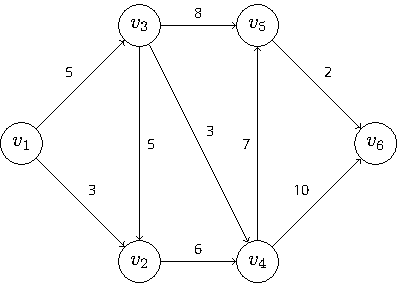
\includegraphics[width=.3\textwidth]{optinum_abb/optinum_5_2_bsp5-1.pdf}
	\end{center}
	
	Jeder minimale Spannbaum hat ein Gewicht von $c = 2+3+3+5+7 = 20$.
\end{beispiel}

\subsection{Algorithmus von \person{Prim} \& \person{Dijkstra}}

Eine alternative Vorgehensweise zur Gewinnung eines minimalen Spannbaums, bei der in jedem Schritt auf den Zusammenhang des Graphen $G_T$ geachtet wird, kann wie folgt beschrieben werden.

\fbox{\textbf{Algorithmus von Prim \& Dijkstra}}
\begin{enumerate}[label=Schritt \arabic*:, leftmargin=*, start=0]
	\item Initialisierung: $T \defeq \emptyset$, $S \defeq \menge{u}$ für ein beliebiges $u \in V$. Für alle $v \in V \setminus \menge{u}$ setze
	\begin{itemize}[nolistsep, topsep=-\parskip]
		\item $h(v) \defeq c(u,v)$, $p(v) \defeq u$ \hspace{1em} falls $\menge{u,v} \in E$
		\item $h(v) \defeq + \infty$ \hspace{1em} sonst
	\end{itemize}
	\item Solange $\card{T} < n -1$: bestimme $v \in V \setminus S$ mit $h(v) = \min\menge{h(t) : t \in V \setminus S}$ und setze $T \defeq T \cup \menge{\menge{p(v),v}}$ sowie $S \defeq S \cup \menge{v}$. Für alle $t \in V \setminus S$ mit $\menge{v,t} \in E$ und $c(v,t) < h(t)$ setze $h(t) \defeq c(v,t)$, $p(t) \defeq v$.
\end{enumerate}

Dieser Algorithmus ist ebenfalls ein Greedy-Verfahren und besitzt (bei \enquote{gewöhnlicher} Implementierung) eine Laufzeit von $\mathcal{O}(\card{V}^2)$, jedoch sind bei Verwendung spezieller Datenstrukturen auch bessere Abschätzungen möglich. Beide Algorithmen beginnen mit einer leeren Knotenmenge und fügen in jedem Schritt eine Kante mit minimalem \enquote{Gewicht} ($c$ bzw. $h$) hinzu. Sie unterscheiden sich vor allem darin, wie genau die Auswahl dieser Kante erfolgt und wie die Bildung eines Kreises vermieden wird.

\section{Optimale Wege}

\subsection{Das Kürzeste-Wege-Problem}

Gegeben sei ein gerichteter, gewichteter Graph $G = (V,E,c)$ mit $c(e) \ge 0$ für alle $(u,v) \in E$. Der Wert $c(e)$ kann zum Beispiel als Länge  (oder allgemein \enquote{Kosten}) interpretiert werden.
Es sind nun ausgehend von einem Startknoten $v_1$ ein kürzester Weg zu jedem anderen Knoten $v_k \in V$ zu finden.

\begin{aussage}
	Es existiert eine Bogenmenge $E_w \subseteq E$ mit $\card{E_w} = \card{V} - 1$, die für jeden Knoten $v_k \neq v_1$ einen kürzesten Weg von $v_1$ zu $v_k$ beinhaltet.
\end{aussage}
\begin{proof}
	Weniger als $\card{V} - 1$ Bögen würden einen Widerspruch zum Zusammenhang liefern. Angenommen es gäbe mehr als $\card{V} - 1$ Bögen. Dann existiert ein Knoten $v \neq v_1$ mit (Eingangs-) Grad $\delta^-(v) \ge 2$, d.h. es gibt zwei optimale Wege von $v$ zu $v_1$. Nur einer dieser Bögen, die in $v$ enden, ist erforderlich, um eine Bogenmenge gemäß Aufgabenstellung zu erhalten.
\end{proof}

\begin{folgerung}
	$E_w$ ist zusammenhängend und kreisfrei, also ein (gerichteter) Spannbaum.
\end{folgerung}

Ein konkretes Verfahren zur Lösung dieses Problems liefert der \person{Dijkstra}-Algorithmus. Dabei werden, ausgehend von einem Startknoten $s = v_1$, bereits bekannte kürzeste Wege durch Hinzufügen weiterer Bögen/Kanten verlängert, um somit kürzeste Wege für bisher unerreichte Knoten zu finden.

Hierfür nutzen wir die Notation: Es sei
\begin{itemize}[nolistsep, topsep=-\parskip]
	\item $M$ die Menge der Knoten, zu denen ein kürzester Weg bekannt ist
	\item $p(v_k) = p(k)$ der Vorgängerknoten von $v_k$ auf dem kürzesten Weg zu $v_k$
	\item $d(v_k) = d(k)$ die Länge des (bisher) kürzesten Weges zu $v_k$
\end{itemize}
Schließlich erhalten wir den folgenden Algorithmus:

\fbox{\textbf{Algorithmus von \person{Dijkstra}:}}
\begin{enumerate}[label=Schritt \arabic*:, leftmargin=*, start=0]
	\item Initialisierung: Setze $M \defeq \menge{s}$, $d(s) = 0$ und initialisiere für $v \neq s$
	\begin{equation*}
		p(v) \defeq \begin{cases}
		s & (s,v) \in E \\ 0 & (s,v) \notin E
		\end{cases} 
		\qquad
		d(v) \defeq \begin{cases}
		c(s,v) & (s,v) \in E \\ +\infty &(s,v) \notin E
		\end{cases}
	\end{equation*}
	\item Bestimme $u \notin M$ mit $d(u) = \min\menge{d(v) : v \notin M}$. Falls $d(u) = +\infty$, dann \texttt{STOP}. Andernfalls setze $M \defeq M \cup \menge{u}$.
	\item Für alle $v \notin M$ mit $(u,v) \in E$: falls $d(v) > d(u) + c(u,v)$ (also ein kürzerer Weg ist gefunden), dann setze $d(v) = d(u) + c(u,v)$ und $p(v) = u$.
	\item Falls $M \neq V$, gehe zu Schritt 1. Sonst \texttt{STOP}.
\end{enumerate}

Offenbar terminiert dieser Algorithmus nach endlich vielen Schritten, da in jeder Iteration entweder ein Element zu $M$ hinzugefügt wird oder der Algorithmus gänzlich abbricht (Schritt 1). Somit wird Schritt 1 höchstens $\mathcal{O}(n)$ mal ausgeführt und bewirkt dabei höchstens $\mathcal{O}(n)$ Durchläufe der in Schritt 2 benötigten Schleife. Bei naiver Implementierung besitzt dieser Algorithmus also eine Komplexität von $\mathcal{O}(\card{V}^2)$, es sind aber auch bessere Abschätzungen (z.B. $\mathcal{O}(\card{E} + \card{V} * \log\card{V})$) möglich.

Sei $d_G(s,v)$ sei die Länge eines kürzesten Weges von $s$ nach $v$ in $G= (V,E,c)$. Offenbar gilt $d(v) \ge d_G(s,v)$ für alle $v \in V$, da der Algorithmus zumindest irgendeinen Weg von $s$ nach $v$ findet oder feststellt, dass es keinen solchen gibt (also $d(v) = \infty$).

\begin{aussage}
	Gilt $c(e) \ge 0$ für alle $e \in E$, so gibt $d(v)$ die Länge eines kürzesten Weges von $s$ nach $v$ an.
\end{aussage}
\begin{proof}
	Sobald ein Knoten $u \in V$ zu $M$ hinzugefügt wird, ändert sich $d(u)$ nicht mehr. Es genügt daher den Zeitpunkt zu betrachten, an dem $u$ zu $M$ hinzugefügt wird.
	\begin{induction}
		\ianfang Als erstes wird (in der Initialisierung) $s$ in $M$ aufgenommen und $d(s) = 0$ gesetzt. Wegen $c(e) \ge 0$ für alle $e \in E$ ist dies die Länge eines kürzesten Weges.
		\ischritt Sei nun $u \neq s$ der \enquote{zeitlich} erste Knoten, für den bei Aufnahme in $M$ die strikte Ungleichung $d(u) > d_G(s,u)$ gilt, d.h. bei $u$ mach der Algorithmus den ersten Fehler. Sei $\gamma$ ein tatsächlich kürzester Weg von $s$ nach $u$. Dieser muss mindestens einen Knoten $y$ enthalten, der (noch) nicht zur Menge $M$ gehört. Wegen $s \in M$ gilt $y \neq s$. Wir zeigen nun, dass $d(y) = d_G(s,y)$ gilt. Offenbar gilt gemäß Induktionsvoraussetzung $d(x) = d_G(s,x)$ für alle Vorgänger $x \in M$ von $y$ auf $\gamma$. Wenn ferner $\gamma$ ein kürzester Weg von $s$ nach $u$ ist, dann enthält $\gamma$ auch einen kürzesten Weg von $s$ nach $y$. Sei $x \in M$ nun der direkte Vorgänger von $y$ auf $\gamma$. Bei der Aufnahme von $x$ in $M$ wurde auch die Kante $(x,y) \in E$ geprüft und folglich $d(y)$ auf den korrekten Wert $d_G(s,y)$ gesetzt. Dann gilt
		\begin{equation*}
			d(u) > d_G(s,u = d_G(s,y) + d_G(y,u) = d(y) + d_G(y,u) \follows d(u) > d(y)
		\end{equation*}
		Also hätte un aktuellen Schritt $u$ nicht in $M$ aufgenommen werde dürfen. Widerspruch.
	\end{induction}
\end{proof}

\begin{beispiel}
	Graph
%	(1,2,3)
%	(1,4,2)
%	(1,3,1)
%	(2,4,2)
%	(3,4,1)
%	(4,5,1)
%	(4,6,2)
%	(4,7,1)
%	(5,6,3)
%	(5,8,3)
%	(6,7,1)
%	(7,8,2)

	\begin{tabular}{rccccccccc}
		p = & 0 & $v_1$ & $v_1$ & $v_1$ & $v_4$ & $v_4$ & $v_4$ & \cancel{$v_5$} $v_7$ \\ \hline
		    & $v_1$ & $v_2$ & $v_3$ & $v_4$ & $v_5$ & $v_6$ & $v_7$ & $v_8$ \\ \hline
		d = & \fbox{0} & 3 & \uline{1} & 2 & $\infty$ & $\infty$ & $\infty$ & $\infty$ \\
			&          & 3 &           & \uline{2} & &  & &  \\
			&          & 3 &           &        & 3         & 4 & 3 & \\
			&          &   &           &        & \uline{3} & 4 & 3 & \\
			&          &   &           &        &           & 4 & \uline{3} & 6 \\
			&          &   &           &        &           & \uline{4} &           & 5 \\
	\end{tabular}

	Ein minimaler Weg von $v_1$ nach $v_8$ lautet als
	\begin{equation*}
		v_8 \leftarrow v_7 \leftarrow v_4 \leftarrow v_1
	\end{equation*}
\end{beispiel}


\subsection{Das Längste-Wege-Problem}
\begin{description}
	\item[gegeben:] gerichteter, gewichteter Graph $G = (V,E,c)$ mit beliebiger Funktion $\abb{c}{E}{\R}$
	\item[gesucht:] längste Wege von $s \in V$ zu allen anderen Knoten
	\item[naive Idee:] Dijkstra-Algorithmus für $G' = (V,E,-c)$ --- funktioniert im Allgemeinen nicht, da $-c(e) \ge 0$ nicht erfüllt sein muss
\end{description}

\fbox{\textbf{Algorithmus von \person{Ford}/\person{Moore}:}}
\begin{enumerate}[label=Schritt \arabic*:, leftmargin=*, start=0]
	\item Wähle $s \in V$ als Startknoten und setze $d(s) = 0$, sowie
	\begin{equation*}
		p(v) \defeq \begin{cases}
		s & (s,v) \in E \\ 0 & \text{sonst}
		\end{cases} 
		\qquad
		d(v) \defeq \begin{cases}
		c(s,v) & (s,v) \in E \\ -\infty &\text{sonst}
		\end{cases}
	\end{equation*}
	für alle $s \neq v$. Definiere außerdem $A \defeq \menge{s} \cup \menge{v \in V: (s,v) \in E}$, $B \defeq \emptyset$ und $k \defeq 1$.
	%
	\item Falls $A = \emptyset$ oder $k = \card{V}$, dann \texttt{STOP}.
	\item Für alle $u \in A$ und alle $v \in V$ mit $(u,v) \in E$: falls $d(v) < d(u) + c(u,v)$, dann setze $d(v) = d(u) + c(u,v)$ und $p(v) = u$ sowie $B \defeq B \cup \menge{v}$.
	\item Setze $A = B$, $B = \emptyset$, $k \defeq k+1$ und gehe zu Schritt 1.
\end{enumerate}

Nach Abschluss von Schritt 2 symbolisieren die Mengen $A$ und $B$ diejenigen Knoten, zu denen in der vorherigen bzw. aktuellen Iteration ein längerer Weg gefunden wurde. Das Verfahren von \person{Ford}/\person{Moore} besitzt eine Laufzeit von $\mathcal{O}(\card{V} * \card{E})$ und es kann gezeigt werden:

\begin{aussage}
	Der Algorithmus von \person{Ford}/\person{Moore} ermittelt zu jedem Knoten, der von $s$ erreichbar ist, einen längsten Weg, sofern er mit $A = \emptyset$ terminiert. Andernfalls enthält der Graph Kreise positiver Länge.
\end{aussage}

%Graph: 
%(1,2,1)
%(2,3,2)
%(3,2,3)
%(3,4,4)

Da hierbei die Gewichte $c(e)$ auch negativ sein durften, kann eine modifizierte Variante des Algorithmus zum Auffinden kürzester Wege ich beliebigen Graphen genutzt werden.

\subsection{Netzplantechnik}

%\newcommand{\FAZ}{F\!A\!Z}
%\newcommand{\SAZ}{S\!A\!Z}
Längste Wege sind vor allem dann von Interesse, wenn die Wege eines Graphen eine logische Abfolge von Teilprojekten beschreiben, die erfüllt sein müssen, bevor ein neues Teilprojekt starten kann.

\begin{description}
	\item[Formal:]
	\begin{itemize}[nolistsep, topsep=-\parskip]
		\item Teilprojekte $TP_i$ mit Dauer $D_i$ ($i = 1, \dots, N$)
		\item Bedingungen an die Anfangszeiten $\AZ_i$ der Teilprojekte (\begriff{Koppelbedingungen})
	\end{itemize}
	\item[Zielstellung] minimale Gesamtdauer des Projekts (und kritische Teilprojekte)
\end{description}

Wir betrachten zwei Fälle:
\begin{enumerate}[label=(\arabic*), nolistsep]
	\item $\AZ_j \ge \AZ_i + \tau_{ij}$ mit $\tau_{ij} \ge 0$: Teilprojekt $\TP_j$ darf frühestens $\tau_{ij}$ Zeiteinheiten nach Beginn von Teilprojekt $\TP_i$ starten
	\item $\AZ_j \le \AZ_u + \tau_{ji}$ mit $\tau_{ji} \ge 0$: Teilprojekt $\TP_j$ muss spätestens $\tau_{ji}$ Zeiteinheiten nach Beginn von Teilprojekt $\TP_i$ starten
\end{enumerate}

Modellierung als Graph $G = (V,E,c)$:

\begin{itemize}[nolistsep, topsep=-\parskip]
	\item $V = \menge{1, \dots, N}$ entsprechend Teilprojekten
	\item Füge Bögen (gerichtete Kanten) ein gemäß
	\begin{itemize}
		\item $(i,j) \in E$ mit $c(i,j) = \tau_{ij}$ genau dann, wenn Fall (1) vorliegt
		\item $(j,i) \in E$ mit $c(j,i) = \tau_{ji}$ genau dann, wenn Fall (2) vorliegt
	\end{itemize}
\end{itemize}

Die Länge eines Weges von $a \in V$ nach $b \in V$ gibt nun an, wie viele Zeiteinheiten $\AZ_b$ mindestens nach $\AZ_a$ liegen muss. Die maximale Länge aller Wege in $G$ von $a$ nach $b$ sei $\ell(a,b)$ und legt die frühestmögliche Startzeit von $\TP_b$ fest (relativ zur Startzeit von $\TP_a$).

Ohne Einschränkung sei Knoten $1$ der Projektbeginn mit $\AZ_1 = 0$. Ein Algorithmus, der für jedes $TP$ die frühest- und spätestmögliche Anfangszeit $\FAZ_i$ bzw. $\SAZ_i$ bestimmt, kann wie folgt formuliert werden:

\fbox{\textbf{MPM-Algorithmus}}
\begin{enumerate}[label=Schritt \arabic*:, leftmargin=*, start=1]
	\item Ermittle $\FAZ_i$ für alle $i \in V$ gemäß $\FAZ_i = \ell(1,i)$. Definiere $T \defeq \FAZ_N + D_N$ als minimale Projektdauer.
	\item Ermittle $\SAZ_i$ für alle $i \in V$ gemäß $\SAZ_i \defeq \FAZ_N - \ell(i,N)$.
\end{enumerate}

Die Bestimmung von $\ell(1,i)$ kann mit dem \person{Ford}-\person{Moore}-Algorithmus bewerkstelligt werden. Zur Bestimmung von $\ell(i,N)$ kann dieser Algorithmus ebenfalls genutzt werden, wobei dazu $\ell(N,i)$ in einem Graphen gesucht wird, der alle Bögen umorientiert (sodass $N$ der feste Startknoten wird).

\begin{definition}
	Die Zeit $\PZ_i \defeq \SAZ_i - \FAZ_i$ heißt \begriff{Pufferzeit} von $\TP_i$. Ein Teilprojekt $i$ mit $\PZ_i = 0$ heißt \begriff{kritisch}.
\end{definition}

Eine Verzögerung in einem kritischen Teilprojekt beeinflusst die gesamte Projektdauer.

Ein ausführliches Beispiel wird in der Übung besprochen.

\section{Maximale Flüsse in Graphen}

\subsection{Problemstellung}

Sei $G = (V,E,k)$ ein gerichteter Graph mit \begriff{Kapazitätsschranken} $k_e \ge 0$ für alle $e \in E$. Weiterhin sei $q \in V$ einzige \begriff{Quelle} und $s \in V$ einzige \begriff{Senke}. Ohne Einschränkung seien ale Inputdaten ganzzahlig. Für jedes $v \in V$ definieren wir
\begin{equation*}
	E^+(v) \defeq \menge{e \in E : e = (v,p)} \qquad E^-(v) \defeq \menge{e \in E : e = (p,v)}
\end{equation*}
der ausgehenden und eingehenden Bögen für $v$.

\begin{definition}
	Eine Funktion $\abb{x}{E}{\R}$ heißt \begriff{Fluss}, wenn gilt
	\begin{equation*}
		\begin{aligned}
			0 \le x_e \le k_e \quad (e \in E) \\
			\sum_{e \in E^-(v)} x_e = \sum_{e \in E^+(v)} x_e \quad (v \in V \setminus \menge{q,s})
		\end{aligned}
	\end{equation*}
	Die zweite Bedingung (Flusserhaltung) ist auch als \person{Kirchhoff}'sches Gesetz bekannt.
\end{definition}

Die Flusserhaltung impliziert 
\begin{equation*}
	\sum_{e \in E^+(q)} x_e = \sum_{e \in E^-(1)} x_e \defqe f(x)
\end{equation*}
wobei $f(x)$ die Flussstärke angibt.

\begin{beispiel} \label{beispiel: 5.3}
%	(1,2,0/7)
%	(1,3,5/5)
%	(2,3,0/4)
%	(3,5,0/4)
%	(3,4,5/6)
%	(4,2,0/5)
%	(4,5,0/6)
%	(4,6,5/8)
%	(5,6,0/4)

	Dargestellt ist ein zulässiger Fluss der Stärke $f(x) = 5$. Die Bogenmarkierungen entsprechen dabei \enquote{$x_e / k_e$}. Der angegebene Fluss ist nicht optimal.
\end{beispiel}

Ein geeignetes Hilfsmittel zur Prüfung der Optimalität ist der \begriff{Residualgraph} (\enquote{Restgraph}). Ohne Einschränkung nehmen wir an, dass für alle $(u,v) \in E$ auch $(v,u) \in E$ gilt. Sofern dies nicht a priori erfüllt ist, ergänzen wir diese mit Kapazität $k_{(v,u)} = 0$.

\begin{definition}
	Sei $\abb{x}{E}{\R}$ ein zulässiger Fluss, d.h. insbesondere ist $0 \le x_e \le k_e$ für alle $e \in E$. Für $e = (u,v) \in E$ definieren wir
	\begin{equation*}
		r(e) = r(u,v) \defeq k_e - x_e + x_{(v,u)}
	\end{equation*}
	das \begriff{Residuum} (\enquote{Restkapazität}) von $e$.
	Weiterhin sei
	\begin{equation*}
		E(x) \defeq \menge{e \in E : r(e) > 0}
	\end{equation*}
	die Menge aller Bögen mit positiven Residuum\footnote{nur dort besteht die Möglichkeit der Flusserhöhung für den Gesamtgraphen}. Der \begriff{Residualgraph} ist definiert als 
	\begin{equation*}
		G(x) \defeq (V, E(x), r(e)_{e \in E(x)})
	\end{equation*}
	wobei $r(e)$ eine \enquote{aktualisierte Kapazität} beschreibt.
\end{definition}

\begin{beispiel}[Fortsetzung von \labelcref{beispiel: 5.3}]
	Aus dem oben angegebenen Fluss ergibt sich der folgende Residualgraph $G(x)$:
	%	(1,2,/7)
	%	(3,1,/5)
	%	(2,3,/4)
	%	(3,5,/4)
	%	(3,4,/1)
	%   (4,3,/5)
	%	(4,2,/5)
	%	(4,5,/6)
	%	(4,6,/3)
	%   (6,4,/5)
	%	(5,6,/4)
	
	Offenbar gilt stets $r(e) \ge 0$ für alle $e \in E$. $G(x)$ enthält also all jene Bögen, die die Möglichkeit zur Flussvergrößerung modellieren, ergänzt um einige Rückwärtsbögen zur Verminderung von Flüssen auf bisher zu stark genutzten Verbindungen.
\end{beispiel}

Eine mögliche Vorgehensweise zur Erzeugung eines maximalen Flusses ist der folgende Algorithmus:

\fbox{\textbf{Algorithmus von \person{Ford}-\person{Fulkerson}}}
\begin{enumerate}[label=Schritt \arabic*:, leftmargin=*, start=1]
	\item Initialisierung --- Setze $x_e = 0$ für alle $e \in E$ (oder ein \enquote{besserer Startfluss}).
	\item Konstruiere den Residualgraphen $G(x)$. Wenn $G(x)$ keinen Weg von $q$ nach $s$ mit positiver Flussstärke enthält: \texttt{STOP} (Optimalität)
	\item Finde einen Fluss $x'$ in $G(x)$, d.h. einen Weg von $q$ nach $s$ in $G(x)$ mit positiver Flussstärke $f'$. Aktualisiere $x$ gemäßt $x_e \defeq x_e + x_e'$ für alle $e \in E(x)$. Gehe zu Schritt~2.
\end{enumerate}

Bei ganzzahligen Kapazitäten findet in jedem Durchlauf des Algorithmus eine Flussvergrößerung um mindestens eine Einheit statt (sofern er nicht in Schritt~2 abbricht). Damit terminiert das Verfahren nach endliche vielen Schritten. Diese Anzahl an Schritten kann jedoch proportional zum Optimalwert $f^\ast = f(x^\ast)$ sein.
Darüber hinaus gibt es Beispiele mit irrationalen Eingabedaten, für die der obige Algorithmus nicht abbricht.

\subsection{Algorithmus von \person{Edmonds} \& \person{Karp}}

\begin{description}
	\item[Idee:] grundsätzlich analog zu \person{Ford}/\person{Fulkerson}, aber im Schritt~3 wird jeweils ein Weg von $s$ nach $q$ mit kleinster Bogenzahl ermittelt
\end{description}

Es bezeichne $\delta_x(u,v)$ den Abstand zwischen $u \in V$ und $v \in V$ in $G(x)$, also die Anzahl der Bögen auf einem kürzesten Weg von $u$ nach $v$.

\begin{lemma}
	\label{lemma: 5.5}
	Sei $x'$ ein Fluss, der aus dem Fluss $x$ erhalten wird (durch einen flussvergrößernden Weg $P$ in $G(x)$). Dann gilt
	\begin{equation*}
		\delta_x(q,v) \le \delta_{x'}(q,v) \quad \text{ für alle } v \in V \setminus \menge{q}
	\end{equation*}
\end{lemma}
\begin{proof}
	Angenommen es gilt $\delta_x(q,v) > \delta_{x'}(q,v)$ für mindestens ein $v \neq q$. Ohne Einschränkung wählen wir dasjenige $v$ mit minimalem Wert $\delta_{x'}(q,v)$. Also gilt
	\begin{equation}
		\delta_{x'}(q,u) < \delta_{x'}(q,v) \follows \delta_x(q,u) \le \delta_{x'}(q,u)
		\label{eq: 5.1}
	\end{equation}
	weil $v$ das \enquote{minimale Gegenbeispiel} war. Sei $P'$ ein kürzester Weg von $q$ nach $v$ in $G(x')$ und $u$ der letzte Knoten vor $v$. Dann gilt $\delta_{x'}(q,u) = \delta_{x'}(q,v) - 1$ und folglich wegen \eqref{eq: 5.1} 
	\begin{equation}
		\delta_x(q,u) \le \delta_{x'}(q,u)
		\label{eq: 5.2}
	\end{equation}
	Betrachten wir $x(u,v)$ vor der Flussvergrößerung:
	\begin{enumerate}[label=(\alph*), nolistsep]
		\item $x(u,v) < k(u,v)$: Dann ist $(u,v)$ in $G(x)$ vorhanden und es gilt
		\begin{equation*}
			\delta_x(q,v) \le \delta_x(q,u) + 1 \overset{\eqref{eq: 5.2}}{\le} \delta_{x'}(q,u) + 1 = \delta_{x'}(q,v)
		\end{equation*}
		im Widerspruch zur Annahme.
		\item $x(u,v) = k(u,v)$: Dann ist $(u,v)$ nicht in $G(x)$ enthalten, wohl aber $(v,u)$. Da jedoch $P'$ den Bogen $(u,v)$ wieder nutzt, muss dieser in $G(x')$ vorkommen. Das geht nur dann, wenn der flussvergrößernde Weg $P$ (der zum Fluss $x$ gehörte) den Bogen $(v,u)$ enthielt (um somit $x'(u,v) < k(u,v)$ und $(u,v) \in G'(x)$ zu bewirken). Man erhält
		\begin{equation*}
			\delta_x(q,v) \le \delta_x(q,u) - 1 \overset{\eqref{eq: 5.2}}{\le} \delta_{x'}(q,u) < \delta_{x'}(q,v)
		\end{equation*}
		im Widerspruch zur Annahme.
	\end{enumerate}
\end{proof}

Der Algorithmus von \person{Edmonds} und \person{Karp} besitzt eine polynomielle Laufzeit für beliebige (nichtnegative) Kapazitäten.

\begin{lemma}
	Der Algorithmus führt höchstens $\mathcal{O}(\card{V} * \card{E})$ Flussvergrößerungen durch.
\end{lemma}
\begin{proof}
	Jede Flussvergrößerung wird durch einen kritischen Bogen charakterisiert, d.h. auf jedem Weg $P$ gibt es einen Bogen $(u,v)$ mit $r_x(u,v) = \min\menge{r_x(e) : e \in P}$, der die Erhöhung des Flusses am meisten beschränkt. Gemäß Konstruktion verschwindet ein kritischer Bogen im nächsten Schritt aus dem Restgraphen. 
	
	\textbf{Frage:} Wie oft kann ein Bogen $(u,v)$ kritisch werden?  
	Ein kritischer Bogen $(u,v)$ kann in einem späteren Restgraphen wieder auftreten, wenn zuvor $(v,u)$ auf einem flussvergrößernden Weg liegt. Sei $x^0$ ein Fluss, bei dem $(u,v)$ kritisch war. Dann gilt $\delta_{x^0}(q,v) = \delta_{x^0}(q,u) + 1$. Ausgehend von $x^0$ betrachten wir nun die vom Algorithmus erzeugte Folge der Flüsse
	\begin{equation*}
		x^0 \to x^2 \to \dots \to x^t \to \dots \to x^k \qquad (t \neq 0, t \neq k, k \ge 2)
	\end{equation*}
	wobei $(u,v)$ in $x^0$ kritisch ist und das nächste Mal in $x^k$; außerdem wird $(v,u)$ in $x^t$ genutzt. Nun gilt
	\begin{equation*}
		\begin{aligned}
		\delta_{x^k}(q,v) = \delta_{x^k}(q,u) + 1 \overset{\text{\cref{lemma: 5.5}}}{\ge} \delta_{x^t}(q,u) + 1 = \delta_{x^t}(q,v) + 2 \overset{\text{\cref{lemma: 5.5}}}{\ge} \delta_{x^0}(q,v) + 2 
		\end{aligned}
	\end{equation*}
	Also gilt: zwischen zwei Wegen, in denen $(u,v)$ kritisch ist, wächst der Abstand zur Quelle um mindestens zwei Einheiten. Ein solcher Abstand kann höchsten $\mathcal{O}(\card{V})$ Einheiten betragen. Demzufolge kann ein Bogen auch höchstens $\mathcal{O}(\card{V})$ Mal kritisch werden. Insgesamt gibt es höchstens $\mathcal{O}(\card{V} * \card{E})$ Flussvergrößerungen.
\end{proof}

Dies impliziert:
\begin{aussage}
	Der Algorithmus besitzt eine Komplexität von $\mathcal{O}(\card{V} * \card{E}^2)$
\end{aussage}

\begin{beispiel}
%	(1,2,2/5)
%	(1,3,5/5)
%	(2,4,2/6)
%	(3,4,5/5)
%	(3,5,0/4)
%	(4,5,2/2)
%	(5,6,2/4)
%	(4,6,5/5)
Wir betrachten den folgenden Graphen

	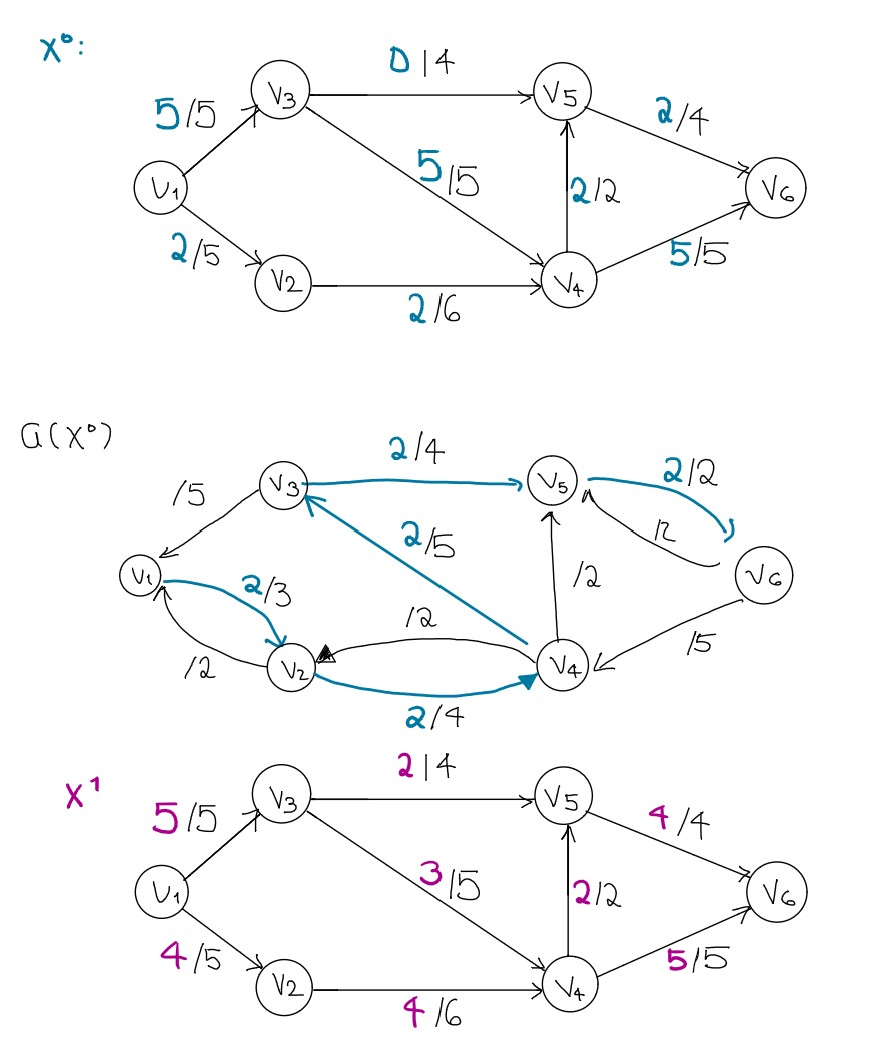
\includegraphics[width=.3\linewidth]{./optinum_abb/optinum_5_4_bsp5-5.jpg}

Flusstärke $= 7$
\end{beispiel}

\end{document}